%!TEX program = xelatex
\documentclass[a4paper,openany]{scrbook}
\usepackage[all,cmtip]{xy}
\usepackage{amsthm}
\usepackage{tilmansdef}
\usepackage{tikz}
\usepackage{enumitem}
\usetikzlibrary{matrix,arrows,decorations,cd}


\usepackage{fontspec,xunicode}
%\setmainfont[Mapping=tex-text,
%	SmallCapsFont={Copperplate},
%	SmallCapsFeatures={Letters=SmallCaps}]{Georgia}
%\setmathrm[Mapping=tex-text]{Georgia}
%\setsansfont[Mapping=tex-text]{Helvetica Neue}
%\setmonofont[Mapping=tex-text]{Andale Mono}
\usepackage[colorlinks]{hyperref}



\usepackage{stmaryrd}

\DeclareMathOperator{\Vect}{Vect}
\DeclareMathOperator{\Open}{Open}
\DeclareMathOperator{\Cov}{Cov}
\DeclareMathOperator{\Der}{Der}
\DeclareMathOperator{\Pic}{Pic}
\DeclareMathOperator{\Princ}{Princ}
\DeclareMathOperator{\chr}{char}
\DeclareMathOperator{\SL}{SL}
\DeclareMathOperator{\stab}{stab}

\DeclareMathOperator{\codim}{codim}
\DeclareMathOperator{\rk}{rk}
\DeclareMathOperator{\Rat}{Rat}
\DeclareMathOperator{\ord}{ord}
\DeclareMathOperator{\divisor}{div}
\DeclareMathOperator{\tw}{tw}

\renewcommand{\C}{\mathcal C}
\newcommand{\nerve}{\mathcal N}

\newcommand{\exterior}{\bigwedge\nolimits}
\newcommand{\chapterauthor}[1]{\hfill\emph{#1}\par\noindent}

\newtheorem{warning}[equation]{Warning}
\subject{\textsc{Lecture Notes}}
\title{Characteristic classes in topology, geometry, and algebra}
\author{Tilman Bauer}
\date{\today{}}
\publishers{Kungliga Tekniska Högskolan, Stockholm, Sweden}


\begin{document}
\frontmatter
\maketitle

\mainmatter

\chapter{Introduction}

Vector bundles can be thought of as vector spaces parametrized by a base space, where ``space'' can mean a topological space, an algebraic variety, or a manifold. They occurence is abundant in topology, geometry, and algebra. Characteristic classes are cohomological invariants of vector bundles and the most important and powerful tools to study them. This course is an advanced level course on characteristic classes in topology, algebra, and geometry, including an introduction to vector bundles, cohomology, and differential geometry.

The course goal is to understand and be able to apply the concept of characteristic classes in a range of mathematical disciplines. At the end of the course, the student will be able to follow current research literature and, if desired, pursue own research projects in this area.



\tableofcontents

\chapter{Vector bundles}

The theory of vector bundles can be described as linear algebra parametrized by a base space. The aim of this chapter is to make this slogan precise and give three equivalent but quite distinct definitions of what a vector bundle is. All three of these definitions have their advantages and disadvantages.

A vector bundle is, roughly speaking, an assignment of a vector space $E_x$ to every point $x \in B$ of some topological space $B$. The space $B$ is called the \emph{base space}, and $E_x$ is the \emph{fiber at $x$} of the vector bundle. This assignment should satisfy two central conditions:

\begin{description}
\item[Continuity:] The fibers $E_x$ should vary continuously with the base point.
\item[Local triviality:] Over small open subsets $U \subset B$ of the base space, we should have $E_x = E_y$ for all $x$, $y \in U$.
\end{description}

The reader should be aware that both of these conditions make no mathematical sense as stated.

\section{Bundles as spaces over a base space}

Let $B$ be a topological space. A \emph{space over $B$} is another topological space $E$ together with a map $p\colon E \to B$. We denote the category of spaces over $B$ by $\Top/B$. Here, a morphism from $p\colon E \to B$ to $p'\colon E' \to B$ is a map $f\colon E \to E'$ such that the triangle
\[
\begin{tikzpicture}
	\matrix (m) [matrix of math nodes, column sep=2ex,row sep=3ex]
	{
		E & & E'\\
		& B\\
	};
	\path[->,font=\scriptsize]
	(m-1-1)	edge node[auto]{$f$} 	(m-1-3)
			edge node[auto,swap]{$p$}	(m-2-2)
	(m-1-3)	edge node[auto]{$p'$}	(m-2-2);
\end{tikzpicture}
\]
commutes, i.~e. such that $p' \circ f = p$. We denote the set of morphisms over $B$ by $\map_B(E,E')$. If $E$, $E' \in \Top/B$, we also define the \emph{fiber product} $E \times_B E' \in \Top/B$ to be
\[
E \times_B E' = \{(e,e') \mid p(e) = p'(e')\} \xrightarrow{(e,e') \mapsto p(e)} B
\]
It is customary to suppress the projection map $p$ in the notation and denote the fiber $p^{-1}(x)$ of $x \in B$ by $E_x$.

\begin{remark}
	In order for the following definition to make sense, we need to restrict attention to a convenient category $\Top$ of topological spaces, i.e.\ one that has well-behaved mapping spaces $\map(Y,Z)$ that satisfy the adjunction $\Hom(X \times Y,Z) \cong \Hom(X,\map(Y,Z))$. The category of compactly generated, weak Hausdorff spaces satisfies this condition, and without further mentioning it, we will assume all topological spaces to belong to this class. 
\end{remark}	

\begin{defn}
Let $B$ be a topological space and $k$ a topological field (typically $\R$ or $\CC$). A \emph{$k$-vector space over $B$} consists of:
\begin{itemize}
\item a space $E \in \Top/B$,
\item a map $s_0\in \map_B(B,E)$, called the zero section,
\item a map $+\in \map_B(E \times_B E,E)$, called addition, and
\item a map $\cdot\in \map_B(k \times E,E)$, called scalar multiplication
\end{itemize}
such that for each $x \in B$, $E_x$ becomes a $k$-vector space with zero $s_0(x)$, addition $+|_{E_x}$, and scalar multiplication $\cdot|_{E_x}$.

A morphism of vector spaces over $B$ is a map $f\in \map_B(E,E')$ compatible with $s$, $+$, and $\cdot$. In particular, $f|_{E_x}$ is a vector space homomorphism for all $x$.
\end{defn}

The most obvious $k$-vector space over $B$ is the product space $k^n \times B$, where the projection to $B$ is simply the projection onto the second factor of the product.

\begin{remark}
	The category-minded reader may observe that a $k$-vector space over $B$ is the same thing as a vector space internal to the category $\Top/B$. 
\end{remark}

\begin{defn}[local triviality of vector bundles]
Let $E$ be a $k$-vector space over $B$. Then $E$ is called a \emph{$k$-vector bundle} if every $x \in B$ has a neighborhood $U \subset B$ such that $E_U = p^{-1}(U)$ is isomorphic to a product space $k^n \times U$ as $k$-vector spaces over $U$, for some $n \geq 0$. The category of $k$-vector bundles over $B$ is denoted by $\Vect_k(B)$ or just $\Vect(B)$ if $k$ is understood or irrelevant. A morphism of $k$-vector bundles is simply a morphism of the underlying $k$-vector spaces over $B$.
\end{defn}

%I would put a comment about how the continuity condition stated before is satisfied.
%% TB: I don't understand what you mean by that.


In a vector bundle $E \in \Vect(B)$, the dimension of each fiber $E_x$ must be finite, but it may vary with $x$. If it does not, and is constantly $n$, we say that $E$ is \emph{equidimensional} of dimension $n$. We denote the subcategory of $n$-dimensional vector bundles on $B$ by $\Vect^n(B)$.

\begin{lemma}
If $B$ is connected then any $E \in \Vect(B)$ is equidimensional.
\end{lemma}
\begin{proof}
For $n \in \N_0$, let $U_n = \{ x \in B \mid \dim E_x = n\}$. By the local triviality condition, each $U_n$ is open and closed, the $U_n$ are disjoint, and they cover $B$. Thus $B=U_n$ for some $n$, and $U_i = \emptyset$ for $i \neq n$.
\end{proof}

So far, the only vector bundles we have encountered are trivial vector bundles (product bundles). It is thus time for some more interesting examples.

\begin{example}[The Möbius strip] \label{exa:mobiusstrip}
Let $E = \R \times [0,1]/\mathord\sim$, where the equivalence relation $\sim$ is generated by $(x,0) \sim (-x,1)$. There is a map $p\colon E \to B = [0,1]/\{0,1\} \cong \S^1$ defined by $p(x,t) = t$. Then $E$ is a $1$-dimensional real vector bundle (a \emph{line bundle}) over $B$, an infinite cylinder with a half twist. The bundle $E$ is known as the \emph{Möbius strip}.

Explicitly, the zero section is given by $s_0(t) = (0,t)$, addition by
\[
(x,t) + (y,t) = (x+y,t)
\]
and scalar multiplication by
\[
\lambda \cdot (x,t) = (\lambda x,t).
\]
Note that the addition is well-defined. 

\begin{figure}[h]
\begin{center}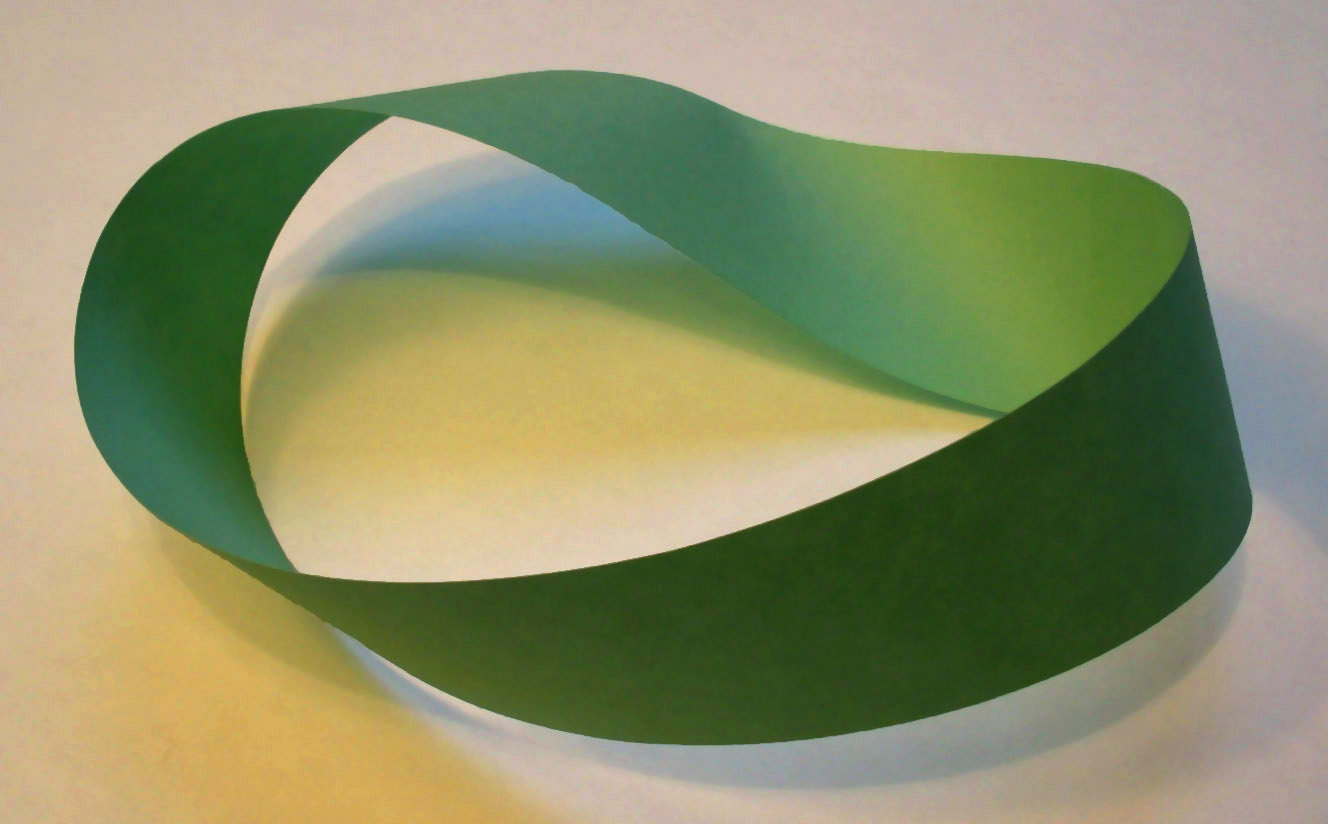
\includegraphics[width=5cm]{mobius.jpg}\end{center}
\caption{The Möbius strip $E$}
\end{figure}

To verify local triviality, let us first consider a point $t \neq \overline 0 \in B$, where $\overline 0$ denotes the equivalence class of $0=1$. Then we can choose a neighborhood $U \ni t$ such that $\overline 0 \not\in U$ and $E_U \xrightarrow{(x,t) \mapsto (x,t)} \R \times U$ is a well-defined isomorphism of vector spaces over $U$. On the other hand, for $t = \overline 0$, choose $U = B-\{\frac12\}$ and define
\[
E_U \xrightarrow{(x,t) \mapsto \begin{cases} (x,t); & t<\frac12\\ (-x,t); & x>\frac12\end{cases}} \R \times U
\]
This is also a an isomorphism of vector spaces over $U$, so we are done.

The Möbius strip is a nontrivial line bundle. This can be seen by observing that the total space of a trivial line bundle falls apart into two components when one removes the zero section, whereas the Möbius strip stays connected.
\end{example}

\begin{example}[Projective space and the tautological bundle] \label{exa:tautological-bundles}
Let $k$ be any field or skew field (typically $\R$, $\CC$, or the quaternions $\mathbf H$) and $P^n = kP^n$ the $n$-dimensional projective space over $k$. This is defined to be the quotient space
\[
P^n = \left(k^{n+1}-\{0\}\right)/\sim,
\]
where the equivalence relation $\sim$ is given by $(x_0,\dots,x_n) \sim (\lambda x_0,\dots,\lambda x_n)$ for $\lambda \in k^\times$. We will think of $P^n$ as the set of lines through the origin in $k^{n+1}$,
\[
P^n = \{ L \subseteq k^{n+1} \mid L \text{ one-dimensional subspace}\},
\]
although this description does not imply what topology we want to have on $P^n$.
We now define the \emph{tautological line bundle} $\mathcal O(-1)$ on $P^n$ by
\[
E = \{ (x,L) \mid L \in P^n, x \in L\}.
\]
It is called tautological because the fiber $E_L$ over a line $L \in P^n$ \emph{is that line}. The notation $\mathcal O(-1)$ will become clear later (Section~\ref{sec:firstchern}). The total space $E_n$ is topologized as a subspace of $k^{n+1} \times P^n$, and the projection map is the obvious one, mapping $(x,L)$ to $L$. Much as in Example~\ref{exa:mobiusstrip}, we see that the vector-space-over-$P^n$ structure of the $(n+1)$-dimensional trivial vector bundle $k^{n+1} \times P^n$ restricts to the subspace $E$, and it remains to show local triviality.

Choose an arbitrary scalar product $\langle \cdot,\cdot \rangle$ on $k^{n+1}$, let $L \in P^n$ be a line in $k^{n+1}$, $x_0 \in L$ a point of norm $1$, and choose $U = \{ L' \in P^n \mid L,L' \text{ are not orthogonal}\}$. Then there is a bijective map
\[
\phi\colon E_U \to k \times U, \quad \phi(x,L) = (\langle x,x_0\rangle,L)
\]
which constitutes a local trivialization of the tautological bundle near $L$.
\end{example}

\begin{example} \label{exa:coordinatecross}
We give an example of a vector space over $B$ which is not locally trivial and hence not a vector bundle. Let $E=\{(x,b) \in \R^2 \mid xb=0\} \xrightarrow{(x,b) \mapsto b} \R = B$ be the projection of the coordinate cross to the $b$-axis. Then
\[
E \times_B E = \{(x_1,x_2,b) \mid x_1=x_2=0 \text{ if } b\neq 0\} \xrightarrow{(x_1,x_2,b) \mapsto (x_1+x_2,b)} E
\]
gives $E$ the structure of a real vector space over $B$ (the scalar multiplication is defined similarily). However, no neighborhood $U$ of $0 \in B$ has $E_U \cong U \times \R^n$ for any $n$ since the fiber over $0$ is $1$-dimensional, while all other fibers are $0$-dimensional.
\end{example}

According to the definition, an isomorphism of vector bundles is a map $f\in \map_B(E,E')$ of vector spaces over $B$ which has an inverse $g\in \map_B(E',E)$. The following characterization is less obvious than one might at first think:

\begin{thm} \label{thm:fiberwiseiso}
A map of vector bundles $f\in \map_B(E,E')$ is an isomorphism of vector bundles iff $f|_{E_x}\colon E_x \to E'_x$ is an isomorphism on the fibers for every $x \in B$.
\end{thm}
\begin{proof}
The “only if” direction is obvious, so assume that $f$ induces a vector space isomorphism on all fibers. Then $f$ is bijective and has an inverse map $f^{-1}\colon E'_x \to E_x$, but is $f^{-1}$ continuous?

To show this, we will use local trivializations. Let $x \in B$ have a trivializing neighborhood $U \subset B$ for both $E$ and $E'$ and $\phi\colon E_U \to k^n \times U$, $\phi'\colon E'_U \to k^n \times U$ be local trivializations. The restriction $f|_{E_U}$ can be written as the composition of maps over $U$,
\[
f|_{E_U}\colon E_U \xrightarrow{\phi} U \times k^n \xrightarrow{G} U \times k^n \xrightarrow{(\phi')^{-1}} E'_U
\]
for some map $G \in \map_U(U \times k^n,U \times k^n)$, which by linearity over $U$, must be of the form
\[
G(u,x) = (u,g(u)x) \quad \text{for some $g\colon U \to k^{n \times n}$}.
\]
In fact, since $f_{E_u}$ is an isomorphism, $g$ has to take values in $\GL_n(k)$.

But then we have that $f^{-1}|_{E'_U} = \phi^{-1} \circ (\id \times g^{-1}) \circ \phi'$, where $g^{-1}$ denotes the pointwise matrix inverse $u \mapsto g(u)^{-1}$, not the inverse map. As a composite of continuous maps, $f^{-1}|_{E'_U}$ is therefore continuous at $x$. 
\end{proof}

\begin{exer} \label{exer:complement-of-tautological-bundle}
Consider the spaces $kP^n$ from Example~\ref{exa:tautological-bundles} again. Choose a scalar product on $k^{n+1}$ and define an $n$-dimensional vector bundle on them by
\[
E = \{(x,L) \mid L \in kP^n,\; x \in L^\perp\}.
\]
That is, the point $x$ is in the hyperplane orthogonal to $L$. Shows that this defines a vector bundle, which we will call $\mathcal O(-1)^\perp$.
\end{exer}

\begin{exer}
Let $k=\R$, $\CC$, or $\mathbf H$. Show that there is a homeomorphism between $kP^1$, the one-dimensional projective space over $k$, and $\S^{\dim_\R(k)}$, i.~e. $\S^1$, $\S^2$, and $\S^4$, respectively.

Show that the Möbius bundle $\mu$ of Example~\ref{exa:mobiusstrip} is isomorphic to the tautological line bundle $\mathcal O(-1)$ on $\R P^1$.
\end{exer}

\section{Bundles as sheaves} \label{sec:bundlesassheaves}

\begin{defn}
Let $p\colon E \to B$ be a vector bundle and $U \subseteq B$. Then we define the set of \emph{sections} of $p$ to be
\[
\Gamma_p(U) = \map_U(U,E_U) = \{s\colon U \to E \mid p \circ s = \id_U\}.
\]
\end{defn}
Using the vector space structure over $B$ of $E$, we can define an addition and scalar multiplication on $\Gamma_p(U)$,
\[
(s+s')(u) = s(u)+s'(u), \quad (\lambda s)(u) = \lambda \cdot s(u),
\]
so that $\Gamma_p(U)$ is actually a (usually infinite-dimensional) $k$-vector space. Loaning a term from algebraic geometry, $\Gamma_p$ is actually a \emph{sheaf} of $k$-vector spaces.

\begin{defn}
Let $B$ be a topological space. Let $\Open(B)$ be the category whose objects are the open subsets $U \subseteq B$ and which has precisely one morphism $U \to U'$ iff $U \subseteq U'$. Then a contravariant functor $F$ from $\Open(B)$ to sets (or spaces, groups, $k$-vector spaces) is called a \emph{presheaf} (of spaces, sets, groups, or $k$-vector spaces). That is, $F$ assigns to each open $U$ a set (space, group, vector space) $F(U)$, often called the sections of $F$ over $U$, and for each inclusion $U \subseteq U'$ there is a map (homomorphism, linear map) $F(U') \to F(U)$, usually denoted by $s \mapsto s|_U$. This assignment of maps is required to be transitive for double inclusions $U \subseteq U' \subseteq U''$ and $F$ must map the identity inclusion $U = U$ to the identity.

A \emph{morphism of presheaves} is a natural transformation of functors. In other words, a morphism $f\colon F \to G$ consists of morphisms $f(U)\colon F(U) \to G(U)$ for each $U \in \Open(B)$ such that for any inclusion $V \subseteq U$ in $\Open(B)$, $f(U)(s)|_V = f(V)(s|_V)$.

A presheaf $F$ on $B$ is called a \emph{sheaf} if it satisfies the \emph{gluing condition}: if $U \subseteq B$ is covered by open sets $\{U_\alpha\}_\alpha$ and we are given, for each $\alpha$, a section $s_\alpha \in F(U_\alpha)$ in such a way that on intersections $U_{\alpha\beta} = U_\alpha \cap U_\beta$, we have that
\[
s_\alpha|_{U_{\alpha\beta}} = s_\beta|_{U_{\alpha\beta}},
\]
then there exists a unique section $s \in F(U)$ such that $s|_{U_\alpha} = s_\alpha$ for all $\alpha$. In words, if we have separate sections over each element of the open cover, and they match up on intersections, then we can glue them together to obtain a section on all of $U$.

A morphism of sheaves is just a morphism of the underlying presheaves; in other words, sheaves are a full subcategory of presheaves.
\end{defn}

It should come as no surprise that sections of a bundle actually form a sheaf:

\begin{prop}
Let $p\colon E \to B$ be a $k$-vector bundle. Then $\Gamma_p$ is a sheaf of $k$-vector spaces on $B$.
\end{prop}
\begin{proof}
We begin by showing that $\Gamma_p$ is a presheaf. Given an inclusion $U \subseteq U'$, we have a canonical restriction map
\[
\Gamma_p(U') = \{s \colon U' \to E \mid p \circ s = \id\} \xrightarrow{-|_U} \{s \colon U \to E \mid p \circ s = \id\} = \Gamma_p(U),
\]
and the functoriality is obvious. Now let us check the gluing condition. Let $U_\alpha$ be an open cover of $U$ and $s_\alpha \in \Gamma_p(U_\alpha)$ such that $s_\alpha|_{U_{\alpha\beta}} = s_\beta|_{U_{\alpha\beta}}$. Then we define $s \in \Gamma_p(U)$ by
\[
s(x) = s_\alpha(x) \quad \text{if } x \in U_\alpha
\]
This is defined on all of $U$ because $\{U_\alpha\}$ covers $U$, and it is well-defined by the matching condition on intersections. Furthermore, $s$ is the only element of $\Gamma_p(U)$ which restricts to $s_\alpha$ on all $U_\alpha$ because if there was another $s' \in \Gamma_p(U)$, being a different function, it would have to disagree with $s$ on some point $x$ which lies in some $U_\alpha$, but we must have $s(x) = s_\alpha(x) = s'_\alpha(x) = s'(x)$.
\end{proof}

\begin{example}
A particular case is the sheaf $\mathcal O_B$ of sections of the trivial line bundle $k \times B$ over $B$. In this case we have that $\mathcal O_B(U)$ is just the set of continuous functions from $U$ to $k$, and this is in fact a sheaf of $k$-algebras, where the multiplication is given pointwise. We will sometimes omit the index and just write $\mathcal O$ for this sheaf when the base space is obvious.
\end{example}

If $R$ is a sheaf of rings (or $k$-algebras) on a space $X$ then an \emph{$R$-module sheaf $M$} is a sheaf of abelian groups (or $k$-vector spaces) with an action
\[
R(U) \times M(U) \to M(U),
\]
natural in $U$, that makes $M(U)$ an $R(U)$-module for all $U$. A \emph{morphism of $R$-module sheaves} $f\colon M \to N$ is a morphism of sheaves such that for every $U$, $f(U)\colon M(U) \to M(U)$ is an $R(U)$-module homomorphism.

\begin{prop}
Let $p\colon E \to B$ be a $k$-vector bundle. Then $\Gamma_p$ is a sheaf of $\mathcal O_B$-modules. Moreover, $\Gamma_p$ is \emph{locally free}, i.~e. if for every $x \in B$ there exists a neighborhood $U \ni x$ such that $\Gamma_p|_U \cong \mathcal O_U^n$ for some $n \geq 0$.
\end{prop}
\begin{proof}
The action
\begin{align*}
\mathcal O_B(U) \times \Gamma_p(U) =& \map(U,k) \times \map_U(U,E_U) = \map_U(U,k\times E_U)\\
\xrightarrow{\map_U(U,\cdot)} &\map_U(U,E_U) = \Gamma_p(U)
\end{align*}
gives $\Gamma_p$ the desired structure.

To show local freeness, let $x \in B$ and choose a trivializing neighborhood $U \ni x$ with $\phi\colon E_U \xrightarrow{\sim} k^n \times U$. Then for any $V \subseteq U$, we have $\Gamma_p(V) \cong \Gamma_{k^n \times U}(V) \cong \mathcal O_U(V)^n$, hence $\Gamma_p$ is indeed locally free.
\end{proof}

It is natural to ask whether the sheaf of sections associated to a vector bundle suffices to completely describe the vector bundle, and moreover, whether any sheaf of vector spaces can be realized as the sections of some vector bundle. The best way to formulate this is by an equivalence of categories.

\begin{thm}\label{thm:vbsheafequivalence}
The functor
\[
\Vect(B) \xrightarrow{p \mapsto \Gamma_p} \{\text{finitely generated locally free $\mathcal O$-module sheaves on $B$}\}
\]
is an equivalence of categories.
\end{thm}

In order to give an inverse construction, we need in particular to extract the fiber over a single point $b \in B$ from a sheaf $F$.

\begin{defn}
The \emph{stalk at $b \in B$} of a sheaf on $F$ is
\[
F_b = \colim_{U \in \Open_b(B)} F(U),
\]
where $\Open_b(X)$ denotes the poset of open sets in $X$ containing $b$, considered as a subcategory of $\Open(X)$ (cf. Appendix~\ref{app:limits} for the definition of a colimit in a category).

If $s \in F(U)$ is a section and $b \in U$ then the natural map $F(U) \to F_b$ sends $s$ to an element $s_b \in F_b$, which is called the \emph{germ} of $s$ at $b$.
\end{defn}

Since $F_b$ is defined using the restriction maps of the sheaf $F$, the stalk of a sheaf $F$ inherits whatever additional structure $F$ has: the stalk of a sheaf of groups is a group, the stalk of a sheaf of $k$-vector spaces is a $k$-vector space, etc. Furthermore, taking stalks is functorial, i.~e. a morphism of sheaves induces a morphism of stalks.

\begin{example}
Let $B$ be a space and $\mathcal O$ the sheaf of continuous functions on $B$. Then the stalk $\mathcal O_b$ consists of \emph{germs of continuous functions at $b$}. Those are function $f$ defined in some neighborhood $U$ of $b$ modulo the equivalence relation generated by
\[
(f,U) \sim (g,V) \quad \text{if} \quad  f|_{U\cap V} = g|_{U\cap V}.
\]
Note the $\mathcal O_b$ has an ideal $(\mathcal O_b)_+$ consisting of those germs of functions that vanish at $b$. This is the kernel of the evaluation map
\[
\mathcal O_b \xrightarrow{s \mapsto s(b)} k,
\]
thus the quotient $\mathcal O_b/(\mathcal O_b)_+$ is isomorphic with $k$.
\end{example}

Given any sheaf $M$ of $\mathcal O$-modules, the stalk $M_b$ is a module over $\mathcal O_b$. We define the \emph{fiber} of $M$ at $b$ to be the quotient
\[
\overline M_b = M_b / (\mathcal O_b)_+M_b.
\]
This is a $k$-vector space in a natural way, and it is finite-dimensional if $M$ was finitely generated.

\begin{lemma}\label{lemma:fiberreconstruction}
Let $p\colon E \to B$ be a vector bundle and $\Gamma=\Gamma_p$ the associated locally free $\mathcal O$-module sheaf. Then for every $b \in B$ there is a natural isomorphism of $k$-vector spaces
\[
\Phi\colon \overline\Gamma_b \to E_b
\]
\end{lemma}
\begin{proof}
Since $\Gamma_b$, $\bar\Gamma_b$, and $E_b$ only depend on an arbitrarily small neighborhood of $b$ in $U$, we may assume that $E = B \times E_b$ is trivial.

The evaluation map $\tilde \Phi\colon \Gamma_b \to E_b \cong k^n$ sends a germ of a continuous function $f\colon U \to k^n$ to its value at $b \in U$. Clearly, it is surjective (we may take $f$ to be constant, for example). Furthermore, the ideal $(\mathcal O_b)_+\Gamma_b$ is contained in the kernel of $\tilde \Phi$. To see the opposite inclusion, let $f\colon U \to k^n$ be in the kernel of $\tilde \Phi$, i.~e., $f(b)=0$. If we write $f=(f_1,\dots,f_n)$ for $f_i \colon U \to k$ then we see that
\[
f = f_1 e_1 + \dots + f_n e_n \in (\mathcal O_b)_+\Gamma_b,
\]
where $e_i\colon U \to k^n$ denote the constant function taking the $i$th standard basis vector of $k^n$ as value, and $f_i$ is considered an element in $(\mathcal O_b)_+$.

Thus the induced map
\[
\Phi\colon \bar \Gamma_b = \Gamma_b/(\mathcal O_b)_+\Gamma_b \to E_b
\]
is an isomorphism.
\end{proof}

Let  $M,N$ be sheaves of $\mathcal O$-modules on the space $B$. Then the set $\Hom_{\mathcal O} (M,N)$ of morphisms of $\mathcal{O}$-modules is a $k$-vector space in a natural way. 

\begin{exer}
	\label{exer:Omodmaps}
	Show that the map $\Hom_{\mathcal O} (\mathcal O,M) \to M(B)$ that sends $\varphi$ to $\varphi(B)(1)$ is a $k$-linear isomorphism. Deduce that $\Hom_{\mathcal O} (\mathcal O^m,M) \cong M(B)^m$.
\end{exer}	

\begin{proof}[Proof of Thm.~\ref{thm:vbsheafequivalence}]
To show that $\Gamma$ is an equivalence of categories, it suffices to show that it is fully faithful and essentially surjective. Let $p\colon E \to B$ and $p'\colon E' \to B$ be two vector bundles on $B$ and $\Gamma$, $\Gamma'$ their associated locally free $\mathcal O$-module sheaves of sections. For the functor $\Gamma$ to be fully faithful in this setting means that the map
\[
\map_B(E,E') \xrightarrow{\Gamma} \Hom_{\Mod_{\mathcal O}}(\Gamma,\Gamma')
\]
is bijective, where the right hand side denotes the set of morphisms of $\mathcal O$-module sheaves.

For injectivity, assume that two maps $f,\; g \in \map_B(E,E')$ induce the same map on the right hand side. By applying the natural transformation $\Phi$ from Lemma~\ref{lemma:fiberreconstruction}, they induce the same maps between the fibers of $\Gamma$ and $\Gamma'$, which are the fibers $E_b \to E'_b$. Thus the maps agree on every fiber, hence $f=g$.

For surjectivity, by Lemma~\ref{lemma:fiberreconstruction} again, any map $f\colon \Gamma \to \Gamma'$ of $\mathcal O$-module sheaves induces maps $f_b\colon E_b \to E'_b$ on every fiber, which almost shows surjectivity, except that we must show that the resulting map $f = \bigcup_{b \in B} f_b$ is continuous.

This can be checked locally, so let us assume that $E = B \times k^m$ and $E' = B \times k^n$ are trivial vector bundles, and correspondingly, $\Gamma = \mathcal O^m$ and $\Gamma' = \mathcal O^n$. By Exercise~\ref{exer:Omodmaps}, $f$ corresponds to a continuous map $B \to \Hom_k(k^m,k^n)$, and evaluation of this map at $b$ gives $f_b$.

For essential surjectivity we must show that every finitely generated locally free $\mathcal O$-module sheaf $M$ on $B$ is isomorphic to $\Gamma_p$ for some vector bundle $p\colon E\to B$. Let $\mathcal U = \{U_\alpha\}_\alpha$ be an open cover of $B$ such that $ M|_{U_\alpha}$ is trivial, i.~e. such that there is an isomorphism
\[
\phi_\alpha\colon  M|_{U_\alpha} \to \mathcal O_{U_\alpha}^{n_\alpha}.
\]
In particular, for every $u \in U_\alpha$, we have a natural homomorphism
\[
\overline \phi_{\alpha,u}\colon M(U_\alpha) \to \overline M_u \to \map(\{b\},k^{n_\alpha}) = k^{n_\alpha}.
\]
Let
\[
\tilde E = \coprod_{\alpha} k^{n_\alpha} \times U_\alpha \xrightarrow{\tilde p\colon (x_\alpha,y_\alpha) \mapsto y_\alpha} B.
\]
We will construct the total space $E$ of the desired vector bundle by gluing the disjoint summands of $\tilde E$ together over all intersections $U_{\alpha\beta}$. Concretely, we define a relation $\sim$ on $\tilde E$ by
\[
(x_\alpha,u_\alpha) \sim (x_\beta,u_\beta) \quad \text{iff} \quad \left\{\begin{matrix}
u_\alpha=u_\beta \in U_{\alpha\beta} \quad\text{ and }\\
\exists s \in M(U_{\alpha\beta})\colon \overline \phi_{\alpha,u_\alpha}(s) = \phi_{\beta,u_\beta}(s).\end{matrix}\right.
\]

Then $E = \tilde E/\sim$. Since only points in different components of the disjoint union are identified, we still have local triviality $E|_{U_\alpha} \cong k^{n_\alpha} \times U_\alpha$. 

We now define a map of sheaves
\[
\Phi\colon M \to \Gamma_p
\]
by using the gluing condition. For $U_\alpha$, we define
\[
\Phi_\alpha\colon M|_{U_\alpha} \xrightarrow{\phi_\alpha} \mathcal O_{U_\alpha}^{n_\alpha} = \Gamma_{\tilde p}|_{U_\alpha} \to \Gamma_p|_{U_\alpha}.
\]
using the local trivializations $\phi_\alpha$. To see that these maps glue, we need to verify that
\[
\Phi_\alpha|_{U_{\alpha\beta}} = \Phi_\beta|_{U_{\alpha\beta}}.
\]
Thus, let $s \in M(U_{\alpha\beta})$ be a section and $u \in U_{\alpha\beta}$. Then $\Phi_\alpha(s)(u) = (\phi_{\alpha,u}(s),u) \sim (\phi_{\beta,u}(s),u) = \Phi_\beta(s)(u)$.
\end{proof}

\begin{remark}
The inverse construction of a vector bundle from a sheaf given above depends heavily on the local trivialization and is therefore not functorial. But this is not needed to show that the functor $\Gamma$ is essentially surjective.
\end{remark}


\section{Bundles as cocycles}
\label{sec:bundlesascocycles}
Let $p\colon E \to B$ be an $n$-dimensional $k$-vector bundle and choose an open cover $U_\alpha$ of $B$ such that each $U_\alpha$ is a trivializing neighborhood, so that we can choose isomorphisms
\[
\phi_\alpha \in \map_{U_\alpha}(E_{U_\alpha},k^n \times U_{\alpha}).
\]

%I've changed g_\alpha\beta from \phi_\beta\phi_\alpha^{-1} to \phi_\alpha\phi_\beta^{-1} to make COC3 work. In what follows I've might have missed changing some indexation. (JH)
Now let $U_{\alpha\beta} = U_\alpha \cap U_\beta$. Then we can compose two such trivializations and obtain an isomorphism
\[
\tilde g_{\alpha\beta}\colon k^{n} \times U_{\alpha\beta} \xrightarrow{(\phi_\beta|_{U_{\alpha\beta}})^{-1}} E_{U_{\alpha\beta}} \xrightarrow{\phi_\alpha|_{U_{\alpha\beta}}} k^{n} \times U_{\alpha\beta}.
\]
Since $\tilde g_{\alpha\beta}$ is a map over $B$, we can write
\begin{equation}\label{eq:cocycletobundlemap}
\tilde g_{\alpha\beta}(x,u) = (g_{\alpha\beta}(u)(x),u)
\end{equation}
for some continuous function $g_{\alpha\beta}\colon U_{\alpha\beta} \to \map(k^{n},k^{n})$. Furthermore, since $\tilde g_{\alpha\beta}$ is a linear isomorphism on fibers, we actually have that $g_{\alpha\beta}\colon U_{\alpha\beta} \to \GL_{n}(k)$. Conversely, for any open subset $U$ of $B$ and any map $g_{\alpha\beta}\colon U \to \GL_n(k)$, we denote by $\tilde g_{\alpha\beta}\in \map_{U}(k^n \times U,k^n \times U)$ the map defined by \eqref{eq:cocycletobundlemap}.

\begin{lemma} \label{lemma:vectorbundlegivescocycle}
Let $p\colon E \to B$ be a $k$-vector bundle with a trivializing open cover $\{U_\alpha\}_\alpha$ and change-of-coordinates maps $g_{\alpha\beta}\colon U_{\alpha\beta} \to \GL_{n}(k)$ for each pair $(\alpha,\beta)$. Then we have:
\begin{enumerate}[label=\normalfont \bfseries{(COC\arabic*)},leftmargin=*]
\item $g_{\alpha\alpha} \equiv I_n$; \label{it:coc1}
\item $g_{\alpha\beta} = g_{\beta\alpha}^{-1}$; \label{it:coc2}
\item $g_{\alpha\beta} g_{\beta\gamma} g_{\gamma\alpha} \equiv I_n$ on $U_{\alpha\beta\gamma}$. \label{it:coc3}
\end{enumerate}
\end{lemma}

\begin{proof}
  Let us consider $\tilde g_{\alpha\beta}$ as maps $U_{\alpha\beta} \to \GL_n(k)$. For \ref{it:coc1} we have $(g_{\alpha\alpha}(u),u) = \tilde g_{\alpha\alpha}(u) =  \phi_\alpha^{-1} \phi_\alpha(u) \equiv (I_n,u)$.
Condition \ref{it:coc2} is actually redundant and follows from \ref{it:coc1} and \ref{it:coc3} since
\[
I_n \underset{\text{(COC3)}}\equiv g_{\alpha\beta} g_{\beta_\alpha} g_{\alpha\alpha} \underset{\text{(COC1)}} = g_{\alpha\beta} g_{\beta_\alpha}.
\]
 Finally for \ref{it:coc3},
\[
  (g_{\alpha\beta}(u) g_{\beta \gamma}(u) g_{\gamma\alpha}(u),u) = \tilde g_{\alpha\beta}(u) \tilde g_{\beta \gamma}(u) \tilde g_{\gamma\alpha}(u) = (\phi_\alpha \phi_\beta^{-1})(\phi_\beta\phi_\gamma^{-1})(\phi_\gamma\phi_\alpha^{-1})(u) \equiv (I_n,u).
\]
\end{proof}


\begin{defn}
Let $G$ be a topological group and $\mathcal U = \{U_\alpha\}_{\alpha \in I}$ an open cover of some space $B$. Then a \emph{cocycle $g$ for $\mathcal U$ with values in $G$} is a family of continuous maps
\[
g_{\alpha\beta}\colon U_{\alpha\beta} \to G \quad (\alpha,\;\beta \in I)
\]
such that \ref{it:coc1}--\ref{it:coc3} hold. We denote the set of cocycles for $\mathcal U$ with values in $G$ by $Z^1_{\mathcal U}(B;G)$.
\end{defn}


A particular kind of cocycle is always easy to construct: given a collection of maps $c_\alpha\colon U_\alpha \to G$, we can define $g_{\alpha\beta}(u) = c_\alpha(u)c_\beta(u)^{-1}$; this obviously satisfies the cocycle conditions. A cocycle of this form is called a \emph{coboundary}. More generally:

\begin{defn} Two cocycles $g$, $g'$ are \emph{cohomologous} if there is collection of maps $c_\alpha\colon U_{\alpha} \to G$ such that $g_{\alpha\beta}' = c_\alpha g_{\alpha\beta} c_\beta^{-1}$. We denote the set of cocycles modulo this equivalence relation by $H^1_{\mathcal U}(B;G)$.
\end{defn}

\subsection{Fiber bundles and principal $G$-bundles}

If vector bundles give rise to cocycles with values in $\GL_n(k)$, it is natural to ask if there is some geometric origin of cocycles with values in other topological groups $G$.

\begin{defn}
	Let $F$ be a space. A \emph{fiber bundle over $B$ with fiber $F$} is a space $E$ over $B$ such that for all $x\in B$ there is an open neighborhood $U$ of $x$ such $E_U \cong U \times F$ as spaces over $U$. We may write $F \to E \to B$.
\end{defn}	

\begin{example}
	An $n$-dimensional vector bundle is a fiber bundle with fiber $k^n$.
\end{example}	

%I changed the left action into a right action. This seems to be more standard in the literature, and the relationship with vector bundles comes out more nicely, as seen in the change-of-coordinate maps. Again I hope I've changed it consistenly throughout. (JH)
\begin{defn}
  Let $G$ be a topological group. A \emph{free and transitive $G$-space over $B$} is a space $E$ over $B$ with a right $G$-action $G \to \map_B(E,E)$ which is free and transitive on each fiber. A map of free and transitive $G$-spaces over $B$ is a map $f\in\map_B(E,F)$ which is $G$-equivariant, i.~e., for each $x \in E$, $f  (x.g) = f(x).g$. 

Consider some fiber $E_b$, a fixed $x \in E_b$, and a map $\psi_x\colon G \to E_b, \psi_x(g) = x.g$. Since the $G$-action is free and transitive on $E_b$, the map $\psi_x$ is a bijection, and thus we can identify $E_b$ with $G$. Furthermore, for any $y \in E_b$ we can write $y.g = (x.h).g=x.(h.g)$, for $h=\psi_x^{-1}(y)$, and therefore we can fiberwise identify any $G$-action with right multiplication in a group $G$.

A \emph{principal $G$-bundle} over $B$ is a free and transitive $G$-space which is locally trivial, i.~e.\ such that every point $x \in B$ has a neighborhood $U \ni x$ such that there exists an isomorphism of free and transitive $G$-spaces over $U$
\[
E_U \to U \times G.
\]
Denote the full subcategory of principal $G$-bundles over $B$ by $\Princ_G(B)$.
\end{defn}

\begin{example}
Consider the projective space $P^n = kP^n$ for $k=\R$, $\CC$, or $\mathbf H$ as a quotient of $E=\{ x \in k^{n+1} \mid \|x\|=1\} \cong \S^{(n+1)\dim_\R k-1}$ and let $G = \{ z \in k \mid \|z\|=1\}$. Clearly, $G$ is a Lie group: $\{\pm 1\}=O(1)$, $\S^1 \cong U(1)$, and $\S^3 \cong SU(2)$ in the three cases. Furthermore, $G$ acts freely and transitively on $E$ over $P^n$ by $z.(x_0,\dots,x_n) = (zx_0,\dots,zx_n)$. The proof that the free and transitive $G$-space $E$ is locally trivial, and hence a principal $G$-bundle, proceeds along the same lines as in Example~\ref{exa:tautological-bundles}.

In the special case $n=1$, the fiber bundles
\[
\S^1 \to \S^3 \xrightarrow{\eta} \S^2 \quad (k=\CC)
\]
and
\[
\S^3 \to \S^7 \xrightarrow{\nu} \S^4 \quad (k=\mathbf H)
\]
are called Hopf fiber bundles. Figure~\ref{fig:hopffib} shows a geometric representation of some of the fibers of $\eta$. Every fiber is a circle, and together, they fill out all of $\S^3$, which is picture as $\R^3$ with an (omitted) point at infinity. One can show that any two fibers of $\eta$ are linked in $\S^3$.
\begin{figure}[ht]\[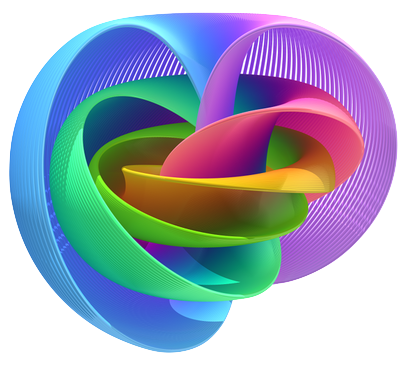
\includegraphics[width=.3\textwidth]{hopffib.png}\]\caption{The Hopf fibration $\eta\colon \S^3 \to \S^2$}\label{fig:hopffib}\end{figure}
\end{example}

\begin{lemma}\label{lemma:princgroupoid}
The category $\Princ_G(B)$ is a groupoid, i.~e., every morphism is an isomorphism.
\end{lemma}
\begin{proof}
  As in the proof of Theorem~\ref{thm:fiberwiseiso}, it suffices to check the isomorphism condition locally, i.~e., we may assume source and target of the morphism $f\colon E \to F$ in $\Princ_G(B)$ are $G \times B$. We have $f(e,b)=(\tau(b),b)$, where $e \in G$ is the identity element, and $\tau$ is a continous map. But then $f(g,b) = f(e,b).g= (\tau(b).g,b)$, and the inverse of $f$ is given by $(g,b) \mapsto (\tau(b)^{-1}.g,b)$.
\end{proof}

\begin{corollary}
A principal bundle with a section is trivial.
\end{corollary}
\begin{proof}
  Given a section $s\colon B \to E$, we can define a morphism $f\colon G \times B \rightarrow E$ between principal $G$-bundles by $f(g,b) = s(b).g$. By Lemma~\ref{lemma:princgroupoid} this is an isomorphism.
\end{proof}

If $\phi\colon G \to \GL_n(k)$ is some homomorphism, then given a principal $G$-bundle $E \to B$ we can define an equivalence relation on $E \times k^n$ by
\[
  (e_1,v_1) \sim (e_2,v_2) \quad \text{iff} \quad (e_1, v_1) = (e_2.g^{-1},\phi(g)(v_2)) \quad \text{for some }g \in G.
\] 
Looking at local trivializations we can see that $(E\times k^n)/_{\sim}$ has a structure of an n-dimensional $k$-vector bundle. We denote this $k$-vector bundle with $E \times_G k^n$, or with $(E \times k^n)/G$. In fact, this construction gives an equivalence of categories between principal $\GL_n(k)$-bundles and $n$-dimensional vector bundles with isomorphisms. For a category $C$, let $C^{\cong}$ denote the subgroupoid with the same objects but only isomorphisms as morphisms. 

\begin{prop}
The functor $\Phi\colon \Princ_{\GL_n(k)}(B) \to (\Vect^n_k(B))^{\cong}$ is an equivalence of groupoids.
\end{prop}
\begin{proof}
Let $p\colon E \to B$ be a vector bundle and define a space $\Psi(E)$ over $B$ by
\[
\Psi(E) = \{(v_1,\cdots,v_n) \in E \times_B \cdots \times_B E \mid v_i \text{ linearly independent over $B$}\}.
\]
Clearly, $\GL_n(k)$ acts freely and fiberwise transitively on $\Psi(E)$, and over a trivializing neighborhood $U$ we have a local trivialization $\Psi(E)_U = \Psi(E_U) \cong \GL_n(k) \times U$. Moreover, $\Psi$ becomes a functor on the subcategory of vector bundle isomorphisms; a non-isomorphism does not preserve the linear independence condition. It is straightforward to see that $\Psi\circ\Phi$ and $\Phi\circ\Psi$ are naturally isomorphic to the identity functors.
\end{proof}

Similarly to vector bundles, a principal $G$-bundle $p\colon E \to B$ with trivializing open cover $\{U_\alpha\}_{\alpha}$ and trivializations $\phi_\alpha\colon E_{U_{\alpha}} \to U_{\alpha} \times G $ gives rise to change-of-coordinate maps $g_{\alpha\beta}\colon U_{\alpha\beta} \to G$ for any $\alpha,\;\beta \in I$ defined by
\[
\phi_\alpha|_{U_\alpha\beta}\left((\phi_\beta|_{U_\alpha\beta})^{-1}(x,\gamma)\right) = (x,g_{\alpha\beta}(x)\gamma) \in G \times U_{\alpha\beta}.
\]
This is well-defined since $\phi_\alpha\phi_\beta^{-1}\colon U_{\alpha \beta} \times G \to U_{\alpha \beta} \times G$ is a map of $G$-bundles, hence preserves right multiplication, and by the fact that a $G$-equivariant map $G \to G$, where $G$ is considered a right $G$-set, is given by left multiplication by some element in $G$.

The following is a straightforward generalization of Lemma~\ref{lemma:vectorbundlegivescocycle} whose proof we leave to the diligent reader:

\begin{lemma}\label{lemma:principalbundlegivescocycle}
Let $G$ be a topological group and $p\colon E \to B$ a principal $G$-bundle with a trivializing open cover $\{U_\alpha\}_{\alpha}$ and change-of-coordinate maps $g_{\alpha\beta}\colon U_{\alpha\beta} \to G$. Then $(g_{\alpha\beta})$ is a cocycle for $\mathcal U$ with values in $G$.

In the case where $G=\GL_n(k)$, this cocycle is equal to the cocycle of the associated vector bundle $\Phi(E)$.\qed
\end{lemma}

\bigskip

The assignment of a cocycle $g$ to a vector bundle or principal $G$-bundle $p$ is not well-defined as it depends both on a choice of trivializing neighborhoods and a choice of trivializations over the latter. The following proposition clarifies, among other things, what happens when we choose different trivializations.

\begin{prop}\label{prop:cocycleisomorphisms}
Let $p\colon E \to B$ and $p'\colon E' \to B$ be two principal $G$-bundles for some topological group $G$. Let $\{U_\alpha\}_\alpha$ be a cover of $B$ that trivializes both $p$ and $p'$, and let $g$ and $g'$ be cocycles associated to $p$ and $p'$, respectively. Then $p \cong p'$ iff and only $g$ and $g'$ are cohomologous.
\end{prop}
Note that one can always find a cover that trivializes both $p$ and $p'$, for instance, by taking all intersections of trivializing neighborhoods of $p$ with trivializing neighborhoods of $p'$.

\begin{proof}
We will show that ``if'' part first, so let us assume that
\[
g'_{\alpha\beta} = c_\alpha g_{\alpha\beta} c_\beta^{-1} \in \map(U_{\alpha\beta},G)
\]
for some collection $c_\alpha\colon U_\alpha \to G$. For $\alpha \in I$, define a map
\[
f_\alpha\colon E_{U_\alpha} \xrightarrow{\phi_\alpha} G \times U_\alpha \xrightarrow{\tilde c_\alpha} G \times U_\alpha \xrightarrow{(\phi_\alpha')^{-1}} E'_{U_\alpha}.
\]
As a composition of three $G$-equivariant maps over $U_\alpha$, it is an isomorphism of principal $G$-bundles over $U_\alpha$. Furthermore, if $U_{\alpha\beta} \neq \emptyset$, we have that

\begin{align*}
f_\alpha \circ f_\beta^{-1} =& (\phi'_\alpha)^{-1} \circ \tilde c_\alpha \circ \phi_{\alpha} \circ (\phi_{\beta})^{-1} \circ \tilde c_\beta^{-1} \circ \phi'_\beta\\
=& (\phi'_\alpha)^{-1} \circ \tilde c_\alpha \tilde g_{\alpha\beta}\tilde c_{\beta}^{-1} \circ \phi'_\beta\\
= & (\phi'_\alpha)^{-1} \circ \tilde g'_{\alpha\beta} \circ \phi'_\beta = \id,
\end{align*}
where all maps are understood as their restriction to $U_{\alpha\beta}$. Thus $f_\alpha|_{U_{\alpha\beta}} = f_\beta|_{U_{\alpha\beta}}$ and thus we can glue these functions together to a globally defined isomorphism of principal $G$-bundles
\[
f\colon E \to E', \quad f(x) = f_\alpha(x) \quad \text{if } x \in U_\alpha.
\]

Now assume that $f\colon E \to E'$ is an isomorphism of principal $G$-bundles. Define $c_\alpha\colon U_\alpha \to G$ by 
\[
\tilde c_\alpha = \phi'_\alpha \circ f \circ \phi_\alpha^{-1}.
\]
Then
\[
\tilde c_\alpha \tilde g_{\alpha\beta} \tilde c_\beta^{-1} = \phi'_\alpha \circ f \circ \phi_\alpha^{-1} \circ \phi_\alpha \circ \phi_\beta^{-1} \circ \phi_\beta \circ f^{-1} \circ (\phi'_\beta)^{-1} =  \phi'_\alpha (\phi'_{\beta})^{-1} = \tilde g'_{\alpha\beta},
\]
hence $g$ and $g'$ are cohomologous.
\end{proof}

Thus for a chosen trivializing cover, the cocycle of a vector bundle or principal $G$-bundle is unique up to cohomology. The following result gives the existence part of the characterization:

\begin{prop}\label{prop:cocycleexistence}
Let $\mathcal U = \{U_\alpha\}_\alpha$ be an open cover on a space $B$ and $(g_{\alpha\beta}) \in Z^1_{\mathcal U}(B;G)$. Then there is a principal $G$-bundle $p\colon E \to B$ and trivializations $\phi_\alpha\in \map_{U_\alpha}(E_{U_\alpha},G \times U_{\alpha})$ whose associated cocycle is $g$.
\end{prop}
\begin{proof}
Let
\[
\tilde E = \coprod_{\alpha} G \times U_\alpha \xrightarrow{p\colon (x_\alpha,y_\alpha) \mapsto y_\alpha} B.
\]
We will construct the total space $E$ of the desired $G$-bundle by gluing the disjoint summands of $\tilde E$ together over all intersections $U_{\alpha\beta}$. Concretely, we define a relation $\sim$ on $\tilde E$ by
\[
  (x_\alpha,u_\alpha)_{\alpha} \sim (x_\beta,u_\beta)_{\beta} \quad \text{iff} \quad u_\alpha=u_\beta \text{ and } g_{\alpha\beta}x_\beta = x_\alpha.
\]
The cocycle conditions (COC1) -- (COC3) are equivalent, in this order, to the reflexivity, symmetry, and transitivity of the relation $\sim$, thus $\sim$ is an equivalence relation, and we define $E = \tilde E/\sim$. Since identifications under $\sim$ only occur within a fiber, $p$ factors through a projection map $p\colon E \to B$.

We now define a $G$-action $G \to \map_B(E,E)$ by
\[
  [(x_\alpha,b)_{\alpha}].\gamma = [(x_\alpha\gamma,b)_{\alpha}].
\]
To see that this is well-defined, observe that for $(x_{\alpha},b)_{\alpha} \sim (x_\beta,b)_{\beta}$, we have
\[
  [(x_\alpha,b)_{\alpha}].\gamma = [(x_\alpha\gamma,b)_{\alpha}] =[(g_{\alpha\beta}x_\beta\gamma,b)_{\alpha}]=[(x_\beta\gamma,b)_{\beta}] = [(x_\beta,b)_{\beta}].\gamma  .
\]
Furthermore, the $G$-action is clearly free and transitive on every fiber. Thus $E$ is a principal $G$-bundle over $B$. Since $g_{\alpha\beta}$ is bijective, $\sim$ identifies distinct points in $G \times U_\alpha$ with distinct points in $G \times U_\beta$, hence the map $G \times U_\alpha \hookrightarrow \tilde E \to E$ is injective with image $E_{U_\alpha}$. We define the local trivialization $\phi_\alpha$ to be the inverse of this map. Then clearly, $g_{\alpha\beta}$ is the change-of-coordinates map associated with $\phi_\alpha$ and $\phi_\beta$, and the proof is complete.
\end{proof}

We can thus define a vector bundle up to isomorphism by specifying a cocycle for some cover. However, maps of vector bundles cannot be described in this way, thus we cannot make a category out of the cocycle description for vector bundles. 

\begin{example}[Real bundles on $\S^1$] \label{exa:bundlesons1}
The circle $\S^1$ has an open cover $\mathcal U_\epsilon = \{U_+,U_-\}$, where $U_+ = \{e^{it} \mid -\pi/2-\epsilon < t < \pi/2+\epsilon\}$ and $U_- = \{e^{it} \mid \pi/2-\epsilon < t < 3\pi/2+\epsilon\}$. The intersection $U_{+,-}$ consists of two small circle segments centered at $i$ and $-i$.  A real-valued cocycle with respect to this cover is given by a single $g\colon U_{+,-} \to \GL_n(\R)$. We want to be able to extend $g$ to the boundary of $U_{+,-}$, which might of course not be possible if $\det(g(u)) \to 0$ as $u \to \partial U_{+,-}$. But we may restrict $g$ to the smaller cover $\mathcal U_{\frac12\epsilon} = \{V_+,V_-\}$ without changing the vector bundle. 
Denote by $V_{\pm i}$ the component of $V_+ \cap V_-$ which contains $\pm i$.

Two cocycles $g$, $g'$ are cohomologous if there are maps $c_\pm\colon V_\pm \to \GL_n(\R)$ such that $g'(x)=c_+(x)g(x)c_-(x)^{-1}$ for $x \in U_{+,-}$.

The Lie group $GL_n(\R)$ consists of two connected components, corresponding to the sign of the determinant. We may, without loss of generality, assume that $\det g(x)>0$ for all $x \in V_i$; if not, we change $g$ cohomologously by choosing constant maps $c_+$ and $c_-$ of determinant $1$ and $-1$, respectively.

Now choose $c_+\colon V_+ \to \GL_n(\R)$ such that $c_+|_{V_i} = g|_{V_i}^{-1}$ and $c_+|_{V_{-i}} =  \id$. This is possible by the connectedness of the space of matrices of positive determinant. Similarily, choose $c_-\colon V_- \to \GL_n(\R)$ such that $c_-|_{V_{-i}} = g|_{V_{-i}}$ and $c_-|_{V_{i}}$ either constant with value the identity matrix, or constant with value $I_- = \begin{pmatrix}-1\\&1\\&& \ddots\\&&&1\end{pmatrix}$, depending on the determinant of $g|_{V_{-i}}$. Then $g' = c_+gc_-^{-1}$ has the following properties:
\begin{itemize}
\item $g'$ is cohomologous to $g$;
\item $g'(x) = \id$ for $x \in V_{-i}$;
\item $g'(x) = \id$ or $g'(x) = I_-$ for $x \in V_{i}$.
\end{itemize}
The $n$-dimensional vector bundle associated with $g$ is either the $n$-dimensional trivial bundle or the Möbius bundle plus an $(n-1)$-dimensional trivial bundle. (What it means to add vector bundles will be explained in more detail in Section~\ref{ssec:whitneysums}.)

This does not quite lead to a classification of all real vector bundles over $\S^1$ since we only consider bundles which are trivial on half-circles.
\end{example}

\begin{exer} \label{exer:bundlesons1}
Classify all real vector bundles on $\S^1$ for arbitrary coverings by trivializing neighborhoods. Hint: use compactness of $\S^1$ to reduce to the case where the cover consists of finitely many overlapping circle intervals.
\end{exer}

\begin{exer} \label{exer:complexbundlesons1}
Show that all complex vector bundles on $\S^1$ are trivial.
\end{exer}

\subsection{Cocycles as functors} \label{subsec:cocyclesasfunctors}

It is useful both conceptually and for what comes later to phrase the definition of a cocycle in the context of \emph{topological categories}. A topological category, or more precisely, a small category object in topological spaces, is an ordinary category where the objects form a set (rather than a proper class) and where both objects and morphism sets carry a topology such that all the structure maps are continuous. We make this more precise in the following definition.

\begin{defn}
Let $C$ be a category, such as the category of topological spaces, that has fiber products. A \emph{category object $\C$ in $C$} is a pair of objects $(\ob \C, \mor \C)$ of $C$ together with morphisms
\begin{itemize}
\item a \emph{unit} $u\colon \ob \C \to \mor \C$;
\item \emph{source} and \emph{target} maps $s$, $t\colon \mor C \to \ob \C$;
\item a composition map $\mu\colon \mor \C \times_{\ob \C} \mor \C \to \mor \C$, where the fiber product denotes the pullback of the diagram
\[
\begin{tikzpicture}
	\matrix (m) [matrix of math nodes, column sep=2ex,row sep=3ex]
	{
		& \mor \C\\
		\mor \C & \ob \C.\\
	};
	\path[->,font=\scriptsize]
	(m-1-2)	edge node[auto]{$t$} (m-2-2)
	(m-2-1)	edge node[auto]{$s$} (m-2-2);
\end{tikzpicture}
\]
\end{itemize}
These morphisms have to satisfy the following axioms:
\begin{description}
\item[(Associativity)] $\mu(\mu(f,g),h) = \mu(f,\mu(g,h))$ for $(f,g,h) \in \mor \C \times_{\ob\C} \mor \C \times_{\ob \C} \mor \C$;
\item[(Identities)] $s\circ u = t \circ u = \id_{\ob \C}$.
\item[(Unitality)] $\mu(f,u \circ s) = f = \mu(u \circ t,f)$ for all $f \in \mor \C$;
\end{description}

A \emph{functor} $F$ between category objects $\C$ and $\D$ in $C$ consists of two morphisms in $C$,
\[
F_0\colon \ob \C \to \ob \D \quad \text{and} \quad F_1\colon \mor\C \to \mor \D,
\]
that are compatible with the unit, source, target, and composition maps. (The reader may spend a minute to think about this compatibility in the case of contravariant functors.)

A \emph{natural transformation} $h\colon \C \to \D$ is a functor
\[
h\colon \C \times [1] \to \D,
\]
where $[1]$ denotes the category with two objects $0$, $1$ and exactly one morphism $0 \to 1$ besides the identity morphisms. We say that the natural transformation goes from the functor $h_0\colon \C \cong \C \times \{0\} \to \D$ to the functor $h_1\colon \C \cong \C \times \{1\} \to \D$.

We call a category object in topological spaces just a \emph{topological category}.
\end{defn}

Note that a category object in sets is just an ordinary category whose objects form a set. (This is called a \emph{small} category.)

A special case of a topological category is a category $\C$ when $\ob\C$ is just a discrete set (but the morphism sets do carry a nontrivial topology). Some authors call this a topological category, rather than our more general definition. An unambiguous name for this kind of category is a \emph{category enriched in topological spaces}.

\begin{example}
If $G$ is a Lie group, such as $\GL_n(k)$ for $k=\R$ or $\CC$, then we can consider $G$ as a topological category with one object $*$ and $\mor = \Hom(*,*) = G$. We will not distinguish in notation between the group $G$ and the one-object category thus defined.
\end{example}

This is the one-object case of the following more general construction:

\begin{example}
If $\{G_n\}_{n \geq 0}$ is a sequence of topological groups, we can define a topological category $\mathcal G$ with objects $\N$ and $\mor \mathcal G = \coprod_{n \geq 0} G_n$, where $G_n = \Hom_{\mathcal G}(n,n)$. This is an example of a topological \emph{groupoid}, i.~e. a category where every morphism is invertible. 
\end{example}

\begin{example} \label{exa:covergroupoid}
Let $\mathcal U = \{U_\alpha\}_{\alpha \in I}$ be an open cover of a space $X$, and let $\mathbf U = \coprod_{\alpha \in I} U_\alpha$. Define the map $p\colon \mathbf U \to X$ to be the standard inclusion on every summand, so that in total, $p$ is an open surjective map.
The pair $(\mathbf U,\mathbf U \times_X \mathbf U)$ becomes a topological category if we define
\begin{itemize}
\item $u\colon \mathbf U \to \mathbf U \times_X \mathbf U$ by $u(x) = (x,x)$;
\item $s(x,y) = x$ and $t(x,y) = y$;
\item $\mu\colon (\mathbf U \times_X \mathbf U) \times_{\mathbf U} (\mathbf U \times_X \mathbf U) = \mathbf U \times_X \mathbf U \times_X \mathbf U \to \mathbf U \times_X \mathbf U$ by $(x,y,z) \mapsto (x,z)$.
\end{itemize}
This is in fact a groupoid as well. We denote it by $\mathbf U$.
\end{example}

\begin{prop} \label{prop:cocyclesasgroupoidmaps}
Let $\mathcal U$ be an open cover of $X$ with associated groupoid $\mathbf U$, and $G$ a topological group, considered as a topological groupoid with one object. Assume that every set in the open cover $\mathcal U$ is connected. Then the natural map
\[
\Fun(\mathbf U,G) \to Z^1_{\mathcal U}(X,G), \quad F \mapsto g \quad \text{where } g_{\alpha\beta} = F_1|_{U_{\alpha\beta}}
\]
is a bijection.

Furthermore, two cocycles are cohomologous if and only if their associated functors are naturally isomorphic.
\end{prop}
\marginpar{I don't think we need the connectivity assumption here. The Prop.\ also seems to be used without this assumption in Cor.\ 3.4.4.}
\begin{proof}
  For $x\in X$ and $U_{\alpha} \cap U_{\beta} \neq \emptyset $, let us denote with $x_{\alpha\beta} \in U_{\alpha\beta}$ a morphism for which $p(x_{\alpha\beta})=x$.
  Since the functor satisfies $F_1(\mu(f,g)) = \mu(F_1(f),F_1(g))$, we can verify the cocyle axioms by applying $F_1$ to the trivial identities 
  \[ 
      \mu(x_{\alpha\alpha},x_{\alpha\alpha}) = x_{\alpha\alpha},  \quad \mu(x_{\alpha\beta},x_{\beta\alpha}) = x_{\alpha\alpha}, \quad \mu(x_{\alpha\beta},x_{\beta\gamma}) = x_{\alpha\gamma}, 
  \] 
  to obtain \ref{it:coc1}, \ref{it:coc2}, \ref{it:coc3}, respectively.
  Conversely, any cocycle defines a functor $F=(F_0,F_1$) by setting $F_1=\coprod_{\alpha} g_{\alpha\beta}$, and $F_0$ is a trivial morphism since $G$ is a one-object category. 

  Now let $h\colon \mathbf U \times [1] \to G$ be a natural transformation from a functor $h_0=F$ to a functor $h_1=F'$, and let $g$ and $g'$ be the cocycles associated to $F$ and $F'$, respectively. Define $c_\alpha\colon U_\alpha \to G$ by $c_\alpha = h|_{U_{\alpha\alpha} \times \{0\to 1\} }$. We want to show that
\[
g_{\alpha\beta}' = c_\beta g_{\alpha\beta} c_\alpha^{-1} \in G \quad \text{for all } \alpha,\beta \in I \text{ such that } U_{\alpha\beta} \neq \emptyset.
\]
This can be reformulated as $g'_{\alpha\beta}c_\alpha = c_\beta g_{\alpha\beta}$. This follows from the functoriality of $h$ because the above identity is the image under $h$ of the true identity
\[
(x \in U_{\alpha\beta},1 \to 1) \circ (x \in U_{\alpha\alpha},0 \to 1) = (x \in U_{\beta\beta},0\to 1) \circ (x \in U_{\alpha\beta},0 \to 0) \text{ in } \mathbf U \times [1].
\]

Conversely, if $g$ and $g'$ are cohomologous by $c_\alpha\colon U_\alpha \to G$ then we define a natural transformation $h$ on morphisms of the form $(U_{\alpha\alpha}, 0 \to 1 )$ by $ h= \coprod_{\alpha}c_{\alpha}\colon \mathbf U \to G$.
\end{proof}

Encouraged by this proposition, we will extend the definition of cocyles with values in a topological groupoid $\mathcal G$ and write $Z^1_{\mathcal U}(X;\mathcal G)$ for the set of functors $\Fun(\mathbf U,\mathcal G)$ and call two such cocycles cohomologous if the associated functors are naturally isomorphic. We also write $H^1_{\mathcal U}(X;\mathcal G)$ for the set of cocycles modulo cohomology.

The following corollary is a straightforward consequence of Propositions~\ref{prop:cocycleisomorphisms}, \ref{prop:cocycleexistence}, and \ref{prop:cocyclesasgroupoidmaps}:
\begin{corollary} \label{cor:cocycleidentification}
There is a bijection
\[
\{\text{$k$-vector bundles on $B$ with trivializing cover $\mathcal U$}\}/\text{iso} \leftrightarrow H^1_{\mathcal U}(B;\coprod_{n \geq 0} \GL_n(k)).
\]
\end{corollary}

We will pursue the cocycle characterization of vector bundles further in Chapter~\ref{ch:cohomology} and also clarify the terms “cocycle”, “coboundary”, and “cohomologous.”


\section{Operations on bundles}

In this section we study the structure of the set of $k$-vector bundles on a space $X$ and how to build new vector bundles from existing ones, mimicking standard constructions in linear algebra.

\subsection{Pullbacks and pushforwards} \label{subsec:pullback-pushforward}

Given a vector bundle $p\colon E \to B$ and a map $f\colon B' \to B$, the fiber product
\[
f^*E = E \times_B B' = \{(e,b) \in E \times B' \mid f(b) = p(e)\} \xrightarrow{(e,b) \mapsto b} B'
\]
becomes a vector bundle $f^*p$ over $B'$, called the \emph{pullback} of $p$ along $f$. That it is locally trivial is clear since $f^{-1}(U)$ is a trivializing neighborhood for $f^*p$ if $U$ is a trivializing neighborhood for $p$. This construction is functorial in the sense that $g^*f^*(p) \cong (f \circ g)^*(p)$ for maps $B'' \xrightarrow{g} B' \xrightarrow{f} B$.

In terms of $\mathcal O_B$-module sheaves, there are pushforward and pullback functors defined as follows. First, given any sheaf $F$ on $B'$, we can define a sheaf $f_*F$ on $B$ by
\[
(f_*F)(U) = F(f^{-1}U) \quad (U \subset B \text{ open});
\]
this maps sheaves of algebras to sheaves of algebras, and in particular, it makes $f_*\mathcal O_{B'}$ a sheaf of rings on $B$. Moreover, there is a natural map of sheaves of rings
\begin{equation}\label{eq:mapofstructuresheaves}
\mathcal O_{B} \to f_*\mathcal O_{B'}; \quad \mathcal O_B(U) = \map(U,k) \xrightarrow{\phi \mapsto \phi \circ f} \map(f^{-1}U,k) = (f_*\mathcal O_{B'})(U).
\end{equation}
Given a $\mathcal O_{B'}$-module sheaf $F$, the pushforward $f_*F$ is naturally an $f_*\mathcal O_{B'}$-module sheaf and hence, by \eqref{eq:mapofstructuresheaves}, a $\mathcal O_B$-module sheaf.

However, for vector bundles $F$, $f_*F$ is not usually a vector bundle, i.~e., the local freeness condition is violated. For instance the pushforward of the constant sheaf $\R$ along the inclusion $\{0\} \hookrightarrow \R$ is the so-called skyscraper sheaf $S$ with $S(U) = \R$ if $0 \in U$ and $S(U) = 0$ otherwise. In terms of vector spaces over $\R$, this is precisely Example~\ref{exa:coordinatecross}.

For the pushforward along $f$ to preserve all vector bundles, it is necessary and sufficient that the map \eqref{eq:mapofstructuresheaves} makes $f_*\mathcal O_{B'}$ into a vector bundle, i.~e., $\map(f^{-1}U,\R) \cong \map(U,\R)^n$ for some $n$ and sufficiently small open sets $U$. This is satisfied if $f^{-1}U \cong U \times \{1,\dots,n\}$, and thus when $B'$ is a finite covering space of $B$. We have thus proved:

\begin{thm}\label{thm:covpushforward}
If $f\colon B' \to B$ is a finite covering space map of degree $n$ then $f_*$ maps vector bundles of dimension $k$ on $B'$ to vector bundles of dimension $kn$ on $B$.
\end{thm}

The sheaf-theoretic formulation of the pullback of a vector bundle is arguably most easily defined as the sheaf of sections of the pullback bundle associated to the sheaf, i.~e., using the equivalence between locally free $\mathcal O_B$-module sheaves and vector bundles.

\begin{example}
Let $f\colon \S^1 \to \S^1$ be the map of degree~$2$ and $\mu\colon E \to \S^1$ the Möbius bundle. I claim that $f^*\mu$ is the trivial line bundle on $\S^1$. Let us think of the Möbius bundle as defined by $E = \R \times [0,1]\mathord\sim$, where $(x,0) \sim (-x,1)$. Then
\[
f^*E \cong (\R \times \left[0,\frac12\right] \sqcup \R \times \left[\frac12,1\right])/\mathord\sim,
\]
where $(x,\frac12)_1 \sim (-x,\frac12)_2$ and $(x,0)_1 \sim (-x,1)_2$. Here the subscripts denote whether the subscripted pair lies in the first or in the second disjoint summand. This is a cylinder with two half-twists, thus trivial. In fact, the map
\[
\R \times [0,1]/\{0,1\} \to f^*E, \quad (x,t) \mapsto \begin{cases} (x,t)_1; & t \leq \frac12\\(-x,t)_2; & t \geq \frac12\end{cases}
\]
is an isomorphism over $B$.

\end{example}

In general, the pullback functor $f^*$ that sends a sheaf on $B$ to a sheaf on $B'$ is the left adjoint of the pushforward functor $f_*$. For an explicit construction, let $G$ be a sheaf on $B$. Then $f^*G$ is the sheaf associated to the presheaf
\begin{align*}
B' \supset U \mapsto \colim_{f(U) \subset V} G(V)
\end{align*}
where the indexing category of the colimit is those open subsets $V$ that contain $f(U)$. We make this into a sheaf by `sheafification', as explained in Proposition~\ref{prop:sheafification}.


\subsection{Whitney sums} \label{ssec:whitneysums}

The generalization of the direct sum $V \oplus W$ of $k$-vector spaces is the Whitney sum of vector bundles.

\begin{defn}
Given two vector spaces over $B$, $p\colon E \to B$, and $p'\colon E' \to B$, we define the (Whitney) sum $E \oplus E' \to B$ to be the vector space over $B$ given by 
\[
E \times_B E' \xrightarrow{(e,e') \mapsto p(e) = p'(e')} B.
\]
\end{defn}

\begin{lemma}
The Whitney sum of vector bundles $E$, $E'$ is a vector bundle, and if $\dim E = m$ and $\dim E' = n$ then $\dim(E\oplus E') = m+n$.
\end{lemma}

\begin{proof}
We only need to check the local triviality condition. Let $U \subset X$ be a trivializing neighborhood for both $p$ and $p'$. Then
\[
(E \times_B E')_U = E_U \times_U E'_U \xrightarrow{\cong} (U \times k^m) \times_U (U \times k^n) \cong U \times k^{m+n}.
\]
\end{proof}

\begin{example}
We will show that for the Möbius bundle $\mu$ on $\S^1$ of Example~\ref{exa:mobiusstrip}, the Whitney sum $2\mu = \mu \oplus \mu$ is a trivial bundle. For that, we define a global trivialization
\[
\R^2 \times \S^1 \to \mu \oplus \mu, \quad (x,y,t) \mapsto (x \cos \pi t + y \sin \pi t,-x \sin \pi t + y \cos \pi t,t),
\]
where, as before, $\S^1$ is considered as the quotient $[0,1]/\{0,1\}$.
\end{example}

An alternative definition of the Whitney sum in terms of locally free $\mathcal O_B$-module sheaves is implicit in the following Lemma:

\begin{lemma}
For two vector bundles $E$, $E'$ over $B$, we have an isomorphism of sheaves $\Gamma_{E \oplus E'} \cong \Gamma_E \oplus \Gamma_{E'}$.
\end{lemma}
\begin{proof}
\[
\Gamma_{E \oplus E'}(U) = \map_U(U,E_U \times_U E'_U) \cong \map_U(U,E_U) \times \map_U(U,E'_U) \cong \Gamma_E(U) \times \Gamma_{E'}(U).
\]
\end{proof}

\begin{exer}
Let $f\colon \S^1 \to \S^1$ be the map $z \mapsto z^2$ of degree~$2$, and $\mu$ the Möbius bundle on $\S^1$. Then $f_*\mu$ is isomorphic to the Whitney sum $\R \oplus \mu$ of a trivial line bundle and the Möbius bundle over $\S^1$.
\end{exer}

\subsection{Kernels and Cokernels*}

Let $f\colon E \to E'$ be a morphism of vector bundles $E \xrightarrow{p} B$, $E' \xrightarrow{p'} B$. Then we can naively define:
\[
\ker f = \{x \in E \mid f(x)=s'(p(x))\} \quad \text{and} \quad \coker f = E'/\sim,
\]
where $x \sim y$ iff $p'(x) = p'(y)$ and $x-y \in \im f$. Since $x$ and $y$ are in the same fiber by the first condition, the expression $x-y$ in the second expression is well-defined. Since both are fiberwise kernels and cokernels of linear maps, it is clear that $\ker f$ and $\coker f$ are vector spaces over $B$.

\begin{warning}
These constructions of $\ker f$ and $\coker f$ are in general not locally trivial, so are \textbf{not} vector bundles. For instance, let $E=E'=\R\times \R$ be trivial bundles over $\R$, and define
\[
f\colon E \to E'; \quad f(x,b) = (bx,b).
\]
Then both $\ker f$ and $\coker f$ are isomorphic to the vector space over $B$ of Example~\ref{exa:coordinatecross}, which is not locally trivial.
\end{warning}


\begin{exer}
The spaces $\ker f$ and $\coker f$ are vector bundles over $B$ if $f$ has locally constant rank, i.e.\ if $b \mapsto \rk(f_b)$ is locally constant on $B$.
\end{exer}

\subsection{Hom bundles}

Let $M$ and $N$ be vector bundles over $B$ from the sheaf point of view. Define a new sheaf $\Hom(M,N)$ by
\[
\Hom(M,N)(U) = \Hom_{\Mod_{\mathcal O_U}}(M|_U,N|_U).
\]
This is a presheaf by restriction, and the gluing condition is clearly satisfied since $M$ and $N$ are sheaves. Moreover, $\Hom_{\Mod_{\mathcal O_U}}(M|_U,N|_U)$ is an $\mathcal O(U)$-module by the restriction map $\mathcal O(U) \to \mathcal O_U$ from the constant presheaf to $\mathcal O_U$. Local freeness follows from Exercise~\ref{exer:Omodmaps}.

Note that a global section of $\Hom(M,N)$ is precisely a morphism of vector bundles $M \to N$. Thus the Hom bundle is an internal homomorphism object in $\Vect(B)$.

A particular case is the bundle
\[
M^* = \Hom(M,\mathcal O_B),
\]
called the dual vector bundle, whose fibers are the dual vector spaces of the fibers of $M$.

\subsection{Tensor bundles}

The previous constructions give a pattern to how one should define the tensor product $M \otimes N$ of two vector bundles. But instead of treating each such construction separately, we will now develop a general method of lifting functors from vector spaces to vector bundles.

\begin{defn}
An \emph{$(p,q)$-ary continuous functor of $k$-vector spaces} is a functor $F\colon (\Vect_k)^p \times (\Vect_k^\op)^q \to \Vect_k$ from $(p+q)$-tuples of finite-dimensional $k$-vector spaces to finite-dimensional $k$-vector spaces which is continuous in the sense that for
\[
V_1,\dots,V_{p+q}, W_1,\dots,W_{p+q} \in \Vect_k,
\]
\begin{align*}
\Hom_k(V_1,W_1) \times \cdots \times \Hom_k(V_{p},W_{p}) \times \Hom_k(W_{p+1},V_{p+1}) \times \cdots \times \Hom_k(W_{p+q},V_{p+q}) \\
\xrightarrow{F} \Hom_k(F(V_1,\dots,V_{p+q}),F(W_1,\dots,W_{p+q}))
\end{align*}
is continuous, where the sets $\Hom_k(V,W)$ carry the usual finite-dimensional vector space topology inherited from $k$.
\end{defn} 

\begin{prop}\label{prop:continuousfunctorlift}
Given any $(p,q)$-ary continuous functor $F$ of $k$-vector spaces, there is an induced functor
\[
F\colon \Vect_k(B)^p \times (\Vect_k(B)^\op)^q \to \Vect_k(B)
\]
which restricts to $F$ on each fiber.
\end{prop}
\begin{proof}
Let $E_1,\dots,E_{p+q}$ be vector bundles on $B$. Define
\[
F(E_1,\dots,E_{p+q}) = \coprod_{b \in B} F((E_1)_b,(E_2)_b,\dots,(E_{p+q})_b).
\]
Of course, we don't want the disjoint union topology on this space over $B$, but the construction is functorial and restricts to $F$ on each fiber.

For the correct topology around $b \in B$, choose a trivializing neighborhood $U$ containing $b$ for all $E_i$ at once. (Since there are finitely many, this exists.) Let $\phi_i\colon E_i \to k^{n_i} \times U$ be trivializations for $E_i$. Let $\phi_{b,i}\colon k^{n_i} \to (E_i)_b$ be the restriction of $\phi_i$ to the fiber over $b$. Now define a bijection
\[
\Phi\colon F(k^{n_1},\dots,k^{n_{p+q}}) \times U \to F(E_1,\dots,E_{p+q})|_U
\]
by
\[
\Phi(y,b) = T(\phi_{b,1},\dots,\phi_{b,p},\phi_{b,p+1}^{-1},\dots,\phi_{b,p+q}^{-1})(y).
\]
We define a subset $V$ of $F(E_1,\dots,E_{p+q})|_U$ to be open iff $\Phi^{-1}(V)$ is open.

To see that this does not lead to conflicting definitions of open sets on intersections $U \cap U'$, note that the map
\[
F(k^{n_1},\dots,k^{n_{p+q}}) \times (U \cap U') \xrightarrow{\Phi} F(E_1,\dots,E_{p+q})|_{U\cap U'} \xrightarrow{\Phi'} F(k^{n_1},\dots,k^{n_{p+q}})
\]
is continuous because it is $F$ applied to a product of (continuous) change-of-coordinate maps.
\end{proof}

We are now in a position to define the tensor product $E \otimes E'$ of two vector bundles by applying Proposition~\ref{prop:continuousfunctorlift} to the $(2,0)$-ary functor $- \otimes_k -$.

\begin{lemma}
For any line bundle $E$, $E \otimes E^* \cong k \times B$, the trivial bundle.
\end{lemma}
\begin{proof}
The evaluation map $\operatorname{ev}\colon V \otimes V^* \xrightarrow{(v \otimes \phi) \mapsto \phi(v)} k$ on vector spaces induces a map $E \otimes E^* \to k \times B$ of vector bundles. If $V$ is one-dimensional then $\operatorname{ev}$ is an isomorphism, thus so is the induced map on line bundles.
\end{proof}

It follows that the set of isomorphism classes of line bundles on a space $B$ form a group with unit $k \times B$, called the \emph{Picard group} $\Pic_k(B)$ of $k$-line bundles on $B$.

\begin{example}
By Example~\ref{exa:bundlesons1} and Exercise~\ref{exer:bundlesons1}, $\Pic_{\R}(\S^1) \cong \Z/2\Z$, generated by the Möbius bundle.
\end{example}

\subsection{Tensor, symmetric, and exterior powers}

The functor $T^n\colon \Vect_k \to \Vect_k$ given by $V \mapsto V^{\otimes n} = V \otimes_k V \otimes_k \cdots \otimes_k V$ is continuous and $(1,0)$-ary. A homomorphism $f\colon V \to W$ induces a homomorphism $f^{\otimes n}\colon V^{\otimes n} \to W^{\otimes n}$. It is not an additive functor if $n \neq 1$ because, for instance, $T(f+g) = f \otimes f + f \otimes g + g \otimes f + g \otimes g \neq T(f)+T(g)$, but this is not required in order to apply Proposition~\ref{prop:continuousfunctorlift}. We thus get an induced functor
\[
T^n\colon \Vect_k(B) \to \Vect_k(B),
\]
called the $n$th tensor power functor. This functor has an important subfunctor and an equally important quotient functor.

The symmetric group $\Sigma_n$ on $n$ letters acts linearly on the functor $T^n\colon \Vect_k \to \Vect_k$ by permuting the tensor factors: if $\sigma \in \Sigma_n$ and $v = v_1 \otimes \cdots \otimes v_n \in V^{\otimes n}$ then $\sigma.v = v_{\sigma(1)} \otimes \cdots \otimes v_{\sigma(n)}$. Since every element in $V^{\otimes n}$ is a linear combination of elementary tensors like $v$, this defines an action on all of $V^{\otimes n}$, which is also natural with respect to maps $V \to W$.

We define a subfunctor of $T^n$ by
\[
\Sym^n(V) = \{v \in T^n(V) \mid \sigma.v=v \text{ for all } \sigma \in \Sigma_n\},
\]
called the $n$th symmetric power of $V$, and a quotient functor
\[
\exterior^n(V) = T^n(V)/(v-\sigma.v\mid \sigma \in \Sigma_n),
\]
called the $n$th exterior power of $V$. Of course it suffices to restrict to permutations $\sigma$ which are transpositions since those generate all of $\Sigma_n$. The latter definition is actually only correct if $\chr(k) \neq 2$, which need not concern us at the moment since we are mostly concerned with $k=\R$ and $k=\CC$. The following exercise contains the ``correct'' definition.

\begin{exer}
Define $I = \langle v_1 \otimes \cdots \otimes v_n \in T^n(V) \mid v_i=v_j \text{ for some }i\neq j\rangle$. Show that $I$ is a sub-vector space of $T^n(V)$ and that
\[
T^n(V)/I \cong \exterior^n(V)
\]
as long as $\chr(k) \neq 2$.
\end{exer}

The equivalence class of an elementary tensor $v_1 \otimes \cdots \otimes v_n$ in $\exterior^nV$ is denoted by $v_1 \wedge \cdots \wedge v_n$. 

Both functors $\Sym^n$ and $\exterior^n$ are continuous and $(1,0)$-ary, so they induce corresponding constructions on $\Vect_k(B)$.

\subsection{The determinant line bundle}

Let $V$ be a vector space of dimension $n$. Choose a basis $v_1,\cdots,v_n$ of $V$. Then $\exterior^k(V)$ has dimension $n \choose k$: for any $k$-element subset $\{i_1<\cdots<i_k\}$ of $\{1,\dots,n\}$, the element $v_{i_1} \wedge \cdots \wedge v_{i_k}$ is a basis vector for $\exterior^k(V)$. In particular, $\exterior^n(V)$ is one-dimensional. An isomorphism with $k$ is given by
\[
d\colon \exterior^n(V) \xrightarrow{v_1 \wedge \cdots \wedge v_n \mapsto \det(v_1,\cdots,v_n)} k,
\]
where the determinant is to be understood as the determinant of the square matrix with columns $v_i$. 

Now if $V \in \Vect^n_k(B)$ is an $n$-dimensional vector bundle, $\exterior^n(V)$ is a line bundle, called the \emph{determinant line bundle} of $V$ and denoted by $\det(V)$.

The map $d$ of course depends on the choice of basis. If $k=\R$ then in fact, its sign only depends on the orientation of the basis. We can therefore \emph{define} an orientation of a real vector space $V$ as a choice of isomorphism $\R \to \exterior^nV$ up to scaling by positive numbers.

\begin{defn}
An $n$-dimensional real vector bundle $V \in \Vect^n_\R(B)$ is \emph{orientable} if $\det(V)$ is the trivial line bundle. An \emph{orientation} of $V \in \Vect^n_\R(B)$ is an isomorphism of $\det(V)$ with $B \times \R$ up to scaling with positive functions.
\end{defn}

Thus a line bundle is orientable if and only if it is trivial; in particular, the Möbius bundle of Example~\ref{exa:mobiusstrip} and the tautological bundles $\mathcal O(-1)$ on $\R P^n$ of Example~\ref{exa:tautological-bundles} are not orientable.

\section{Tangent and normal bundles}

Many important vector bundles have their natural home on manifolds rather than arbitrary topological spaces. The most important one is probably the tangent bundle of a smooth manifold. We briefly recall the definition of a manifold, but the reader should consult other sources for a more in-depth treatment.

\begin{defn}
A topological space $M$ is called a (topological, real) manifold if it is Hausdorff, its topology has a countable basis (it is ``second-countable''), and every point has a neighborhood homeomorphic to $\R^n$ for some $n$.
\end{defn}

We now return to the point of view of Section~\ref{sec:bundlesassheaves}, where we thought of a vector bundle on a space $B$ as a locally finite-dimensional free sheaf of $\mathcal O_B$-modules.

\subsection{Smooth manifolds}

\begin{defn}
A ring $R$ is called \emph{local} if it possesses a unique maximal ideal, which we will denote by $R_+$ in these notes. A \emph{morphism of local rings} is a ring morphism $f\colon R \to S$ such that $f(R_+) \subseteq S_+$.
\end{defn}

\begin{example}
Fields are local rings, as their unique maximal ideal is $(0)$. The ring of integers is not local since $(p)$ is a maximal ideal for every prime $p$, but the ring $\Z_{(p)}$ of integers localized at $p$ is local with maximal ideal $(p)$. 

The ring $C^0_0$ of germs of continuous functions $\R^n \to \R$ at $0$ is local with maximal ideal the ideal of germs which vanish at $0$. This is true because the quotient ring $C^0_0/(C^0_0)_+$ is isomorphic with $\R$. Similarily, the rings $C^n_0$ of germs at $0$ of $n$-fold continuously differentiable functions, $C^\infty_0$ of smooth (arbitrarily often differentiable) functions, or $C^\omega_0$ of analytic functions.
\end{example}

\begin{defn}
A sheaf $F$ of rings on a space $X$ is called a \emph{local sheaf of rings} if all stalks $F_x$, for $x\in X$, are local rings (with maximal ideal $(F_x)_+$). A space with a local sheaf of rings on it is called a \emph{locally ringed space}.

A morphism of locally ringed spaces $(X,\mathcal O_X) \to (Y,\mathcal O_Y)$ consists of a map $f\colon X \to Y$ together with a morphism of local sheaves of rings on $Y$, $\tilde f\colon \mathcal O_Y \to f_*\mathcal O_X$. 
\end{defn}

Note that a local sheaf of rings is not the same as a sheaf of local rings, i.~e. a sheaf $F$ of rings such that $F(U)$ is local for all $U \in \Open(X)$. This would preclude $C^0$ from being an example.

In sheaf-theoretic terms, one could say that a manifold is a (second countable Hausdorff) space $M$ together with a local sheaf of $\R$-algebras $C^0$ such that the locally ringed space $(M,C^0)$ is locally isomorphic to $(\R^n,C^0$) for some $n$. That sounds like unwarranted complexity since the original definition just required $M$ to be locally homeomorphic with $\R^n$, without the need to refer to sheaves. Indeed, in this case the additional data of local isomorphisms
\[
\tilde f\colon C^0_{\R^n} \to f_*C^0_{U}
\]
just specifies an isomorphism of the sheaf $C^0_U$ with the sheaf of continuous functions on $U$. 
However, this suggests a viable definition of a smooth (or $C^k$-) manifold. Although the definition would make perfect sense, we will ignore $C^k$-manifolds and just consider smooth (=$C^\infty$-) manifolds. 

\begin{defn}
A \emph{smooth structure} on a space $M$ is a local sheaf of $\R$-algebras $C^\infty$ on $M$, called the \emph{structure sheaf}, such $(M,C^\infty)$ is locally isomorphic , as a locally ringed space, to $(\R^n,C^\infty)$ for some $n$. A \emph{smooth manifold} is a second-countable Hausdorff space together with a smooth structure.

A smooth map $M \to N$ between smooth manifolds is a morphism of locally ringed spaces.
\end{defn}

A more classical definition is via charts and atlases, and we will now show that these are equivalent.

\begin{defn}
Let $M$ be a second-countable Hausdorff space. A \emph{chart} on $M$ is a pair $(U,\phi)$ consisting of an open set $U \subset M$ and a homeomorphism $\phi\colon U \to \phi(U) \subset \R^n$ onto an open subset $\phi(U)$ of $\R^n$, for some $n \geq 0$. An \emph{atlas} is a collection $(U_\alpha,\phi_\alpha)_{\alpha \in I}$ such that the $U_\alpha$ cover $M$. An atlas is \emph{smooth} if for each $\alpha$, $\beta \in I$ such that $U_{\alpha\beta} \neq \emptyset$, the map
\begin{equation}\label{eq:coordinatechange}
g_{\alpha\beta}\colon \phi_\alpha(U_{\alpha\beta}) \xrightarrow{\phi_{\alpha}^{-1}} U_{\alpha\beta} \xrightarrow{\phi_\beta} \phi_\beta(U_{\alpha\beta})
\end{equation}
is a diffeomorphism between open subsets of $\R^n$.

Two smooth atlases $(U_\alpha,\phi_\alpha)_{\alpha \in I}$ and $(V_\beta,\psi_\beta)_{\beta \in J}$ are \emph{equivalent} if for every pair $(\alpha,\beta)$ such that $W = U_\alpha \cap V_\beta \neq \emptyset$, the map
\[
\phi_\alpha(W) \xrightarrow{\phi_\alpha^{-1}} W \xrightarrow{\psi_\beta} \psi_\beta(W)
\]
is a diffeomorphism.

A map $f\colon M \to N$ of smooth manifolds is smooth if for every point $x \in M$ such that $(U,\phi)$ is a chart in $M$ with $x \in U$ and $(V,\psi)$ is a chart in $N$ with $f(U) \in V$, the composite
\[
\R^n \xrightarrow{\phi^{-1}} U \xrightarrow{f} V \xrightarrow{\psi} \R^m
\]
is smooth.
\end{defn}

\begin{thm}
Every smooth manifold has a smooth atlas, and that atlas is unique up to equivalence. Conversely, an equivalence class of smooth atlases gives rise to a unique smooth structure.
\end{thm}
\begin{proof}
We begin by constructing a smooth atlas from a manifold $M$ with smooth structure $C^\infty$.

Let $\mathcal U = \{U_\alpha\}_{\alpha \in I}$ be the set of all open subsets of $M$ over which there is an local isomorphism $\Phi_\alpha\colon C^\infty|_{U_\alpha} \to C^\infty_{\R^{n}}$. By assumption, $\mathcal U$ is a cover of $M$. Underlying the morphism $\Phi_\alpha$ there is a homeomorphism $\phi_\alpha\colon U_\alpha \to \R^{n}$, which gives $M$ the structure of a manifold. To see that the coordinate change functions $g_{\alpha\beta}$ of \eqref{eq:coordinatechange} are smooth, observe that they are covered by isomorphisms of local sheaves of rings
\[
\tilde g_{\alpha_\beta}\colon C^\infty_{\phi_\beta(U_{\alpha\beta})} \to (\phi_\beta)_* C^\infty|_{U_{\alpha\beta}} \to (\phi_\beta \circ \phi_\alpha^{-1})_*C^\infty_{\phi_\alpha(U_{\alpha\beta})},
\]
which says that a function on $\phi_{\alpha}(U_{\alpha\beta})$ is smooth iff its composition with $\phi_b\circ\phi_\alpha^{-1}$ is a smooth function on $\phi_\beta(U_{\alpha\beta})$. This happens if and only if $\phi_b\circ\phi_\alpha^{-1}$ is smooth.

Note that we have constructed what is called a ``maximal smooth atlas'': all possible smooth charts are already in $\mathcal U$.

Conversely, let $(U_\alpha,\phi_\alpha)_{\alpha \in I}$ be a maximal smooth atlas on $M$. Using the gluing condition, we define a local sheaf of rings on $M$ as follows: $C^\infty_{U_\alpha} = (\phi_\alpha^{-1})_* C^\infty_{\R^{n}}$. For an intersection $U_{\alpha\beta}$, we must show that 
\[
C^\infty_{U_\alpha}|_{U_{\alpha\beta}} = C^\infty_{U_\beta}|_{U_{\alpha\beta}},
\]
that is,
\[
(\phi_\alpha^{-1})_* C^\infty_{\phi_\alpha(U_{\alpha\beta})} = (\phi_\beta^{-1})_* C^\infty_{\phi_\beta(U_{\alpha\beta})}
\]
but this is the same as showing that
\[
(\phi_\beta\circ\phi_\alpha^{-1})_*C^\infty_{\phi_\alpha(U_{\alpha\beta})} = C^\infty_{\phi_\beta(U_{\alpha\beta})},
\]
which follows from the fact that $\phi_\beta\circ\phi_\alpha^{-1}$ is smooth.
\end{proof}

The main tool to produce smooth manifolds is the implicit function theorem from multi-variable calculus:

\begin{thm}
Let $F\colon U \to \R^N$ be a smooth map, where $U \subseteq \R^{N+n}$ is open. Assume that $0$ is a regular value of $F$, i.~e., the differential $DF(x)$ has maximal rank $N$ at every point $x \in F^{-1}(0)$. Then $F^{-1}(0)$ is a smooth $n$-dimensional submanifold of $\R^{n+N}$.
\end{thm}

\begin{exer}
Verify that the above is indeed the implicit function theorem.
\end{exer}

There are a number of pitfalls for our intuition regarding smooth structures, but the following remarks may help to circumnavigate them.

Let $M = \{ (x,y) \in \R^2 \mid x \geq 0, y \geq 0, xy=0\} \subseteq \R^2$ be the union of the nonnegative $x$- and $y$-axes. Since $M$ has a corner, one might be tempted to assume that $M$ is not a smooth manifold. But all this shows is that $M$ is not a smooth submanifold of $\R^2$, i.~e. that the sheaf $C^\infty_{\R^2}|_M$ is not locally isomorphic to $C^\infty_{\R^1}$. Looking at $M$ as an abstract manifold, it is homeomorphic to $\R^1$ and a smooth structure is given by pulling back $C^\infty_{\R^1}$ along this isomorphism.

Are there, then, any examples of topological manifolds which do not admit any smooth structure at all? This is a nontrivial question which we will answer in \ref{nonsmoothable}. The first example was given by Kervaire \cite{kervaire:nonsmoothable}. However, all manifolds in dimensions less than $4$ are smoothable.

A related question is whether a manifold can have nonisomorphic smooth structures. This was answered affirmatively by Milnor in \cite{milnor:7spheres} where he showed that $\S^7$ admits exactly $28$ nonisomorphic smooth structures, of which only one is the standard structure from the embedding $\S^7 \hookrightarrow \R^8$.

\subsection{The tangent bundle of a smooth manifold}

The sheaf-theoretic definition of a smooth manifold $M$ allows for a concise construction of the tangent bundle.

\begin{defn}
Let $A$ be a $k$-algebra. A \emph{derivation} on $A$ is a $k$-linear function $D\colon A \to A$ such that $D(ab) = D(a)b+D(b)a$ (the so-called \emph{Leibniz rule}). Denote the set of derivations on $A$ be $\Der(A)$; this is an $A$-module.
\end{defn}

Note that $D(1)=0$ since $D(1) = D(1\cdot 1)=2D(1)$.

\begin{example}
Let $A=C^\infty(\R^n)$ be the algebra of smooth real-valued functions on $\R^n$. For a chosen basis of $\R^n$, let $x_i\colon \R^n \to \R$ be the coordinate function $(x_1,\dots,x_n) \mapsto x_i$. Then $\frac\partial{\partial x_i}$ is a derivation on $A$.

In fact, this is a derivation on the quotient algebra $C^\infty_0$ of germs of smooth functions at $0$.
\end{example}

\begin{defn}
Let $M$ be a smooth manifold. Define a sheaf $TM$ by
\[
TM(U) = \Der(C^{\infty}(U)).
\]
\end{defn}

\begin{thm} \label{thm:tangentspacebundle}
For an $n$-dimensional manifold $M$, $TM$ is an $n$-dimensional real vector bundle.
\end{thm}
\begin{proof}
We have to show that $TM$ is a finitely generated, locally free sheaf of $C^\infty_M$-modules. This is a local question, so we may assume that $M = \R^n$. After choosing a basis of $\R^n$, the differential operators $\frac\partial{\partial x_i}$ are linearly independent global sections of $TM$. We will show that the map $(C^\infty_M)^n \to TM$ which sends $(f_1,\cdots,f_n)$ to the derivation $f_1\frac\partial{\partial x_1}+\cdots+f_n\frac\partial{\partial x_n}$ is an isomorphism of $C^\infty_M$-module sheaves. Let $X \in \Der(C^\infty_{\R^n})$ and $f \in C^\infty(\R^n)$. Then for any two points $x$, $p \in \R^n$ we have
\begin{align*}
f(x) = & f(p)+\int_0^1 \frac d {dt} f(tx+(1-t)p)\; dt = f(p) + \int_0^1 \sum_{i=1}^n\left.\frac{\partial f}{\partial x_i}\right|_{tx+(1-t)p} (x_i-p_i)\; dt \\
= & f(p) + \sum_{i=1}^n (x_i-p_i) \int_0^1 \left.\frac{\partial f}{\partial x_i}\right|_{tx+(1-t)p}\; dt.
\end{align*}

Applying $X$ and evaluating at $p$ using the Leibniz rule, we get
\[
X(f)(p) = \sum_{i=1}^n X(x_i-p_i)(p) \left.\frac{\partial f}{\partial x_i}\right|_p.
\]
Since $X(x_i-p_i)(p) = g(p)$ is a real-valued continuous function of $p$, we have shown that $X(f)$ is a linear combination of $\frac{\partial f}{\partial x_i}$.
\end{proof}

\begin{thm}
For any smooth map $f\colon M \to N$ of smooth manifolds, there is an induced map $Tf\colon f_*TM \to TN \in \Vect(N)$ which is functorial in the sense that $T\id=\id$ and $T(f \circ g)=Tf \circ Tg$.
\end{thm}
\begin{proof}
Given $D \in (f_*TM)(U) = \Der(C^\infty_{f^{-1}U})$ for $U \in \Open(N)$, define $Tf(D) \in \Der(C^\infty_U)$ by $Tf(D) = D \circ f$.
\end{proof}

The definition of the tangent bundle is quite abstract and it is maybe not immediately clear that this really carries tangential information. To see that it does, let us compare the tangent bundle with a more obvious construction when $M$ is embedded in $\R^N$.

\begin{defn}
Let $M \subseteq \R^N$ be a smooth submanifold. Define a vector bundle $T^gM \to M$ (the ``g'' stands for ``geometric'') by
\[
T^gM = \Biggl\{(m,v) \in M \times \R^N \Biggm| \begin{matrix}v = \gamma'(0) \text{ for some smooth curve}\\\gamma\colon (-1,1) \to M \text{ with } \gamma(0)=m\end{matrix}\Biggr\}.
\]
\end{defn}
This is obviously a vector space over $M$. Let $n = \dim M$. To verify local triviality, let $x \in M$ and $p\colon \R^N \to V$ be a projection onto an $n$-dimensional subspace $V$ of $\R^N$ such that $p(x)=0$ and $p$ is a chart in a neighborhood $U$ of $x$ in $M$. Now define
\[
\tilde p\colon T^gM|_U \to V \times V; \quad \tilde p(m,v) = (p(m),p(v)).
\]
This is an isomorphism of vector bundles covering the map $p$ and therefore gives a local trivialization.

We now define a map
\[
\Phi\colon \Gamma_{T^gM}(U) \to TM(U)
\]
by $\Phi(s)(f)(x) = D_{s(x)}f$ for $s\colon U \to T^gM|_U$, $f \in C^\infty_U(V)$, $V \subseteq U$ open, and $x \in V$. Here $D_v$ denotes the directional derivative in the direction $v \in \R^N$.

\begin{prop}
The map $\Phi$ is an isomorphism of vector bundles.
\end{prop}
\begin{proof}
It is clear that $\Phi$ is a map of vector spaces over $B$. Since isomorphism can be tested locally, we may assume that $M \cong \R^n \subseteq \R^N$ is the standard embedding.
It suffices to show that $\Phi$ is an isomorphism on the fibers by Theorem~\ref{thm:fiberwiseiso}. Without loss of generality we will consider the fiber over $0 \in \R^n$. But then
\[
\Phi_x\colon \{ \gamma'(0) \mid \gamma\colon (-1,1) \to \R^n, \gamma(0)=0\} = \R^n \to \Der(C^\infty_{\R^n})_0
\]
is an isomorphism by the proof of Theorem~\ref{thm:tangentspacebundle}.
\end{proof}

\begin{exer}
Let $M \subset \R^{n+1}$ be an $n$-dimensional submanifold (a ``hypersurface''). Show that $TM \oplus \R$, Whitney sum of the tangent bundle and a trivial bundle, is trivial. (The ``hairy ball theorem'' from algebraic topology \cite{hatcher:AT} shows that for $M=\S^2 \subset \R^3$, $TM$ is nontrivial. In particular, this provides an example of the counter-intuitive fact that a nontrivial vector bundle can become trivial when a trivial vector bundle is added.)
\end{exer}

\begin{exer}
Show that the tangent bundle of any Lie group is trivial.
\end{exer}

\begin{exer}
Let $M$ be a smooth $n$-dimensional manifold with atlas $(U_\alpha,\phi_\alpha)$. The change-of-coordinates map $g_{\alpha\beta}$ \eqref{eq:coordinatechange} is a diffeomorphism between open subsets of $\R^n$. Let $Dg_{\alpha\beta}$ be its total differential, so that $Tg_{\alpha\beta}(u) =_{\operatorname{def}} Dg_{\alpha\beta}|_{\phi(u)} \in \GL_n(\R)$ for all $u \in U_{\alpha\beta}$. Show that the collection $Tg_{\alpha\beta}\colon U_{\alpha\beta} \to \GL_n(\R)$ is a cocycle, and that its associated vector bundle is isomorphic with $TM$.
\end{exer}

\subsection{Normal bundles of embeddings}

\subsection{The cotangent bundle and differential forms}

Let $M$ be a smooth manifold. Then the cotangent bundle $T^*M$ is the linear dual of the tangent bundle of $M$, that is, $T^*M = \Hom_M(TM,\R \times M)$.

A section of $T^*M$ can be considered a differential $1$-form $\omega$. There is a canonical derivation
\[
d\colon C^\infty_M \to T^*M 
\]
given by $d(f)(D) = D(f)$. Locally, any section of $T^*M$ is a $C^\infty$-linear combination of $df$.

The vector space of differential $i$-forms is the $i$th exterior power of $T^*M$:
\[
\Omega^i(M) = \bigwedge\nolimits^i T^*M.
\]
We define $\Omega^0(M) = C^\infty_M$.

We can extend the derivation $d$ to a chain complex of vector bundles, the \emph{de Rham complex} of $M$,
\[
\Omega^0(M) \xrightarrow{d} \Omega^1(M) \xrightarrow{d} \cdots \xrightarrow{d} \Omega^n(M) \to 0
\]
by inductively defining
\[
d(\omega \wedge \tau) = d(\omega) \wedge \tau + (-1)^{p} \omega \wedge d(\tau)
\]
where $\omega \in \Omega^p(M)$ and $\tau \in \Omega^q(M)$, and decreeing that $d^2=0$.



\section{Bundles with more structure}

When $M$ is a smooth manifolds, it is natural to consider vector bundles that are compatible with this smooth structure, as is modelled by the tangent bundle. To be more precise, we define

\begin{defn}
A \emph{smooth vector bundle} on a smooth manifold $M$ is a locally finitely generated free $C^\infty_M$-module sheaf.
\end{defn}

The forgetful map of local sheaves of rings $u\colon C^\infty_M \to C^0_M$ allows us to construct an ordinary (continuous) vector bundle $E'$ from a smooth vector bundle $E$ by tensoring down:
\[
E' = E \otimes_{C^\infty_M} C^0_M.
\]

We can also interpret this definition in terms of vector spaces over $M$. A \emph{smooth atlas} for a (ordinary, continuous) vector bundle $E \to M$ is a collection of local trivializations $(U_\alpha,\phi_\alpha)_{\alpha \in I}$ such that the associated cocycles
\[
g_{\alpha\beta}\colon U_{\alpha\beta} \to \GL_n(k)
\]
are smooth. A smooth vector bundle is a (continuous) vector bundle together with an equivalence class of smooth atlases much analogously to the definition of a smooth structure on a manifold.

The characterization of additional structure by cocycles is a powerful tool and lets us, among other things, make the following definitions:

\begin{defn}
Let $G$ be a topological group group with a homomorphism $\alpha\colon G \to \GL_n(k)$. Let $E$ be a vector bundle on $B$ classified by a cocycle in $c \in H^1_{\mathcal U}(B,\GL_n(k))$. Then a \emph{$G$-structure} on $E$ is a preimage of $c$ under the map $H^1_{\mathcal U}(B,G) \to H^1_{\mathcal U}(B,\GL_n(k))$.
\end{defn}

Note that a $G$-structure neither needs to exist nor does it need to be unique, as the map $H^1_{\mathcal U}(B,G) \to H^1_{\mathcal U}(B,\GL_n(k))$ is in general neither injective nor surjective.

We record a number of important examples.

\begin{example}
Let $G = \SL_n(\R) \subset \GL_n(\R)$. A $G$-structure is called an \emph{orientation} of a vector bundle. Explicitly, it amounts to a choice of equivalence class of atlases whose transition functions take values in $\SL_n(\R) < \GL_n(\R)$.
\end{example}

\begin{example}
Let $G = O(n) < \GL_n(\R)$. A $G$-structure is called a \emph{Euclidean structure} on a real vector bundle. A \emph{Hermitian structure} on a complex vector bundle, similarily, is a $U(n)$-structure.
\end{example}

We will see later (Cor.~\ref{cor:euclideanstructure}) that any vector bundle can be given a Euclidean resp. Hermitian structure under mild conditions on the topology of the base space.

\begin{example}
Let $G = \{1\}$ be the trivial group. Then a $G$-structure exists (and is unique) if and only if the vector bundle is trivial.
\end{example}

\begin{example}
Let $G = \Spin(n) \to SO(n) < \GL_n(\R)$, where $\Spin(n)$ is the spin group, a double cover of the special orthogonal group $SO(n)$. A $G$-structure on a vector bundle is called a spin structure. It implies both a Euclidean structure and an orientation, but is stronger than both. Spin bundles play an important role in real topological $K$-theory.
\end{example}


\chapter{Lie groups, Grassmannians, and universal bundles}

Let $M \in \R^{n+1}$ be a smooth hypersurface (that is, an embedded $n$-dimensional manifold). Then at any point $x \in M$, the normal bundle $\nu_x M$ is a line in $\R^{n+1}$ and thus can be thought of as a point in $\R P^n$. We thus obtain a map
\[
f\colon M \to \R P^n.
\]
This map is continuous (in fact, even smooth, but we won't be needing this property). Indeed, given some chart $(U,\phi)$ of $M$ around $x$, the tangent space $T_xM$ is spanned by the sections $t_i(x) = \phi^*(\frac{\partial}{\partial x_i}|_x)$ and the ``generalized cross product'' $\tilde g(x) = t_1(x) \wedge \dots \wedge t_n(x)$ is a nonvanishing normal vector to $M$ at $x$. In fact, after choosing an isomorphism $\det T_x(U) \cong \R$, we can normalize this map to get what is called a \emph{Gauss map}
\[
g(x) = \frac{t(x)}{\|\tilde g(x)\|} \colon M \to \S^n,
\]
which is continuous, and $f(x) = \bar g(x)$, where $\bar g$ is the map $g$ composed with the canonical projection $\S^n \to \R P^n$. The map $f$ is a ``classifying map'' because $\nu M \cong f^*(\mathcal O(-1))$: we have described a line bundle by a continuous map to a ``classifying space'' ($\R P^n$) which has a universal line bundle ($\mathcal O(-1)$) over it.

In a similar way, if $M$ is embedded in $\R^N$, its normal bundle will give a map
\[
f\colon M \to G_{N-n}(\R^N),
\]
where $G_n(\R^N)$, the ``Grassmannian manifold'', denotes the set of all $n$-dimensional subspaces of $\R^N$, and similarly its tangent bundle will give a map
\[
t\colon M \to G_n(\R^N).
\]

The aim of this chapter is to study the Grassmannians, provide an alternate description of a classifying space $BG$ of $G$-bundles in full generality (that is, without assuming any specific kind of bundle or that the base space is a manifold). Furthermore, we compare $BG$ to the geometric construction with Grassmannians, and show that, indeed, isomorphism classes of principal $G$-bundles are in one-to-one correspondence with homotopy classes of maps to $BG$.

\section{Bundles from free Lie group actions}

\begin{thm} \label{thm:freeLiegroupaction}
Let $M$ be a smooth manifold with a smooth and free action of a compact Lie group $G$. Then $M/G$ is a smooth manifold, and the projection map $M \to M/G$ is a smooth principal $G$-bundle.
\end{thm}

Now let $G$ be a compact Lie group, acting on a smooth manifold $M$. For $x \in M$, the stabilizer $\stab(x)$ is a closed subgroup of $G$, since it is the fiber of the map $G \to X$ that sends $g$ to $gx$. Thus $G/ \stab(x)$ is again a compact Lie group, and it acts freely and transitively on the orbit $Gx$. By the above theorem, the map
\begin{align*}
Gx \to Gx / (G/\stab(x))
\end{align*}
is a smooth $G/\stab(x)$-bundle. But $G/\stab(x)$ acts transitively on $Gx$, so the base space of this bundle is a point. We have thus shown the following
\begin{corollary}[Orbit-stabilizer theorem]
	The map $G \to X$, $g \mapsto gx$ induces an isomorphism $G/\stab(x) \cong Gx$ of $G/\stab(x)$-bundles.
\end{corollary}	


\section{Stiefel and Grassmann manifolds}

In this section we will construct spaces $G_n(k^N)$ whose points correspond to $n$-dimensional linear subspaces of $k^N$. Obviously, for this to be nonempty, we need that $N \geq n$. These spaces are called \emph{Grassmann manifolds} or just \emph{Grassmannians} after their discoverer, 19th century mathematician Hermann Graßmann. They are in fact compact manifolds (when $k=\R$ or $\CC$) and, more generally, smooth projective varieties for any field $k$.

Closely related is another family of manifolds, the \emph{Stiefel manifolds} $V_n(k^N)$, whose points correspond to $n$-frames in $k^N$. An \emph{$n$-frame} is a sequence $(v_1,\dots,v_n)$ of orthonormal vectors in $k^N$. One can thus think of a point in $V_n(k^N)$ as a point $V \in G_n(k^N)$, i.~e. an $n$-dimensional linear subspace of $k^N$, together with a choice of orthonormal basis of $V$. Forgetting this basis gives a canoncial projection map $V_n(k^N) \to G_n(k^N)$. If one does not want to (or cannot) use a scalar product on $k^N$ to define $V_n$, one can look at \emph{noncompact Stiefel varieties} $V_n^{\operatorname{nc}}$, where one relaxes the requirement of orthonormality to mere linear independence.

Observe that we already know the spaces $V_1(k^N)$ and $G_1(k^N)$ by other names, namely:
\begin{eqnarray*}
V_1(\R^{N}) =& \S^{N-1}\\
V_1(\CC^N) =& \S^{2N-1}\\
G_1(k^N) =& k P^{N-1}.
\end{eqnarray*}
A set of one orthonormal vector in $k^N$ is just a unit vector in $k^N$, hence the first two equations, and a one-dimensional subspace in $k^N$ is a point in $k P^{N-1}$ by definition. The topologies we are about to define on $V_1$ and $G_1$ coincide with the familiar topologies.

We topologize $V_n(k^N)$ and $V_n^{\operatorname{nc}}(k^N)$ as subspaces of a product $k^N \times \cdots \times k^N$ of $n$ copies of $k^N$, and $G_n(k^N)$ is endowed with the quotient topology. That is, we use the straightforward identifications
\begin{align*}
V_n(k^N) = & \{ U \in k^{N \times n} \mid U \text{ has orthonormal columns}\} \\
\subseteq & V_n^{\operatorname{nc}}(k^N) = \{ U \in k^{N \times n} \mid U \text{ has maximal rank}\} \subseteq k^{N \times n}
\end{align*}
to define the topologies.

\begin{lemma}[Gram-Schmidt]
The inclusion map $V_n(k^N) \to V_n^{\operatorname{nc}}(k^N)$ is a homotopy equivalence for $k=\R$ or $k=\CC$.
\end{lemma}
\begin{proof}
The Gram-Schmidt orthonormalization process says that
\[
V_n^{\operatorname{nc}}(k^N) \cong V_n(k^N) \times T_n(k),
\]
where $T_n(k)$ denotes the upper triangular $n\times n$-matrices with positive real diagonal. But $T_n(k)$ is contractible.
\end{proof}

\begin{lemma} \label{lemma:principalfibrationongrassmannian}
The group $O(n)$ of orthogonal $n\times n$-matrices acts freely on $V_n(\R^N)$, and the canonical map $V_n(\R^N)/O(n) \to G_n(\R^N)$ is a homeomorphism. 

The same is true for over $\CC$ if one replaces $O(n)$ by the group $U(n)$ of unitary matrices, or if one replaces $V_n(k^N)$ by $V_n^{\operatorname{nc}})(k^N)$ and $O(n)$ by $\GL_n(k)$.
\end{lemma}
\begin{proof}
The group $O(n)$ acts on the $n$ orthonormal vectors of a point in $V_n(\R^N)$. The fiber of the projection map $V_n(\R^N) \to G_n(\R^N)$ over a point $V \in G_n(\R^N)$ is the set of orthonormal bases of $V$, on which $O(n)$ acts freely and transitively, thus the projection map factors through a homeomorphism $V_n(\R^N)/O(n) \to G_n(\R^N)$. The proof in the complex and noncompact cases is the same.
\end{proof}

Picking the $n$ first columns of an $N\times N$-matrix gives us surjective maps
\[
\phi\colon O(N) \to V_n(\R^N), \quad \phi\colon U(N) \to V_n(\CC^N), \quad \phi\colon \GL_N(k) \to V_n^{\operatorname{nc}}(k^N).
\]

\begin{lemma}\label{lemma:grassstiefelashomogeneousspaces}
Consider the group $O(n) \times O(N-n)$ as the subgroup of $O(N)$ of matrices of the form $\left(\begin{smallmatrix} A & 0\\ 0 & B\end{smallmatrix}\right)$. Then $\phi$ factors through an $O(n)$-equivariant homeomorphism
\[
\overline\phi\colon O(N)/O(N-n) \to V_n(\R^N).
\]
In particular, there is a homeomorphism $\frac{O(N)}{O(n)\times O(N-n)} \to G_n(\R^N)$.

Analogous statements hold in the unitary and noncompact cases.
\end{lemma}
\begin{proof}
The group $O(N)$ acts on $V_n(\R^N)$ by mapping an orthogonal $n$-frame to another such $n$-frame. This action is transitive, and the stabilizer group of a frame $F=(v_1,\dots,v_n)$ is the orthogonal group $O(N-n)$ of the orthogonal complement of the span of $F$. Thus by the orbit-stabilizer theorem, $O(N)/O(N-n) \to V_n(\R^N)$ is a homeomorphism, which moreover is $O(n)$-equivariant.
\end{proof}


\begin{corollary}
For $k=\R$, $\CC$, we have that
\[
G_n(k^N) \cong G_{N-n}(k^N)
\]
\end{corollary}
\begin{proof}
This follows directly from the $G_n(k^N) \cong \frac{O(N)}{O(n) \times O(N-n)}$. Geometrically, the homeomorphism $G_n(k^N) \to G_{N-n}(k^N)$ is given by mapping an $n$-dimensional subspace of $k^N$ to its orthogonal (or unitary) complement.
\end{proof}



\begin{corollary} \label{cor:stiefelgrassmannbundle}\label{thm:grassmannianmanifolds}
The spaces $V_n(k^N)$ and $G_n(k^N)$ are compact smooth manifolds for $k=\R$, $\CC$, and the projection map $p\colon V_n(k^N) \to G_n(V^N)$ is a principal $O(n)$-bundle (for $k=\R$) or $U(n)$-bundle (for $k=\CC$). They have the following real dimensions:
\begin{itemize}
\item $\dim V_n(\R^N) = Nn - {n+1 \choose 2}$;
\item $\dim V_n(\CC^N) = 2Nn - n^2$;
\item $\dim G_n(\R^N) = n(N-n)$;
\item $\dim G_n(\CC^N) = 2n(N-n)$.
\end{itemize}
\end{corollary}

\begin{proof}
Theorem~\ref{thm:freeLiegroupaction} together with Lemma~\ref{lemma:grassstiefelashomogeneousspaces} shows that $V_n(k^N)$ is a smooth manifold, and Theorem~\ref{thm:freeLiegroupaction} with Lemma~\ref{lemma:principalfibrationongrassmannian} shows that $G_n(k^N)$ is a manifold and $p$ is a principal bundle.

The claims about dimensions follow from the facts that $\dim O(n) = {n \choose 2}$ and $\dim U(n) = n^2$.
\end{proof}

To exhibit explicit charts for $G_n(k^N)$, it helps to do a little geometry. Let $V \in G_n(k^N)$ be a point, and let $V^\perp$ be its orthogonal (or unitary) complement. Now consider the set
\begin{equation}\label{eq:grassmanncharts}
U_V = \{ V' \in G_n(k^N) \mid V' \cap V^\perp = 0\}.
\end{equation}
Clearly, $V \in U_V$ and $U_V$ is open. The map
\[
\phi_V\colon \Hom(V,V^\perp) \cong k^{n(N-n)} \to U_V; \quad \alpha \mapsto \{v+\alpha(v) \mid v \in V\},
\]
which can be thought of as sending a homomorphism $\alpha$ to its graph in $k^N = V \oplus V^\perp$, is a homeomorphism.

\subsection{The tautological bundle}

Let $E_n(k^N) = \{ (V,v) \mid V \in G_n(k^N), \; v \in V \} \subseteq G_n(k^N) \times k^N$. The projection $\tau$ to the first coordinate gives a smooth surjection $E_n(k^N) \to G_n(k^N)$.

\begin{prop}
The map $\tau\colon E_n(k^N) \to G_n(k^N)$ is an $n$-dimensional vector bundle.
\end{prop}
\begin{proof}
It is clear from the definition that $E_n(k^N)$ is a vector space over $G_n(k^N)$ and that the dimension is $n$, but we need to show local triviality. Consider the open sets $U_V$ of \eqref{eq:grassmanncharts}. We construct a trivialization over $U_V$ by
\[
\tau^{-1}(U_V) \to U_V \times V; \quad (V',v') \mapsto (V',p(v')),
\]
where $p'\colon V' \to V$ is the orthogonal projection of $V'$ to $V$, which is an isomorphism over $U_V$ since its kernel is $V^\perp$.
\end{proof}

The vector bundle $\tau\colon E_n(k^N) \to G_n(k^N)$ is called the \emph{tautological bundle} because the description of its fibers sounds like a tautology: the fiber of $\tau$ over a point $V \in G_n(k^N)$ is $V$.

\begin{thm}
Let $M \subseteq \R^N$ be an $n$-dimensional smooth submanifold of $\R^N$ and $TM \to M$ its tangent bundle. Then there is a map $f\colon M \to G_n(\R^N)$ such that $TM \cong f^*\tau$.
\end{thm}
\begin{proof}
The map $f$ is defined by $f(x) = T_xM \subseteq \R^N$, where $T_xM$ is the tangent space of $M$ at $x$, considered as a linear subspace of $\R^N$. We thus get a vector bundle map $TM \to f^*\tau$ over $M$ which is a fiberwise isomorphism, hence an isomorphism by Theorem~\ref{thm:fiberwiseiso}.
\end{proof}

\section{Simplicial spaces}\label{sec:simplicial-spaces}

We have seen that the tangent bundle of a manifold embedded in Euclidean space has a “classifying map” to the Grassmannian $G_n(\R^N)$ in the sense that it is the pullback of the tautological bundle along this map. In the rest of this chapter, our aim is to make this construction independent of the embedding in Euclidean space, and to generalize it to arbitrary bundles. This requires the notion of a classifying space for a topological group, which is best understood in the context of \emph{simplicial spaces}.

\begin{defn}
A \emph{simplicial space} (or, more generally a simplicial object in a category $C$) is a functor
\[
X\colon \Delta^\op \to \Top \quad \text{(or $C$)},
\]
where $\Delta$ denotes the category with objects the totally ordered sets $[n] = \{0,\dots,n\}$ and morphisms the monotonic maps. Similarly, an \emph{augmented simplicial space} is a functor
\[
X\colon \Delta^\op_+ \to \Top \quad \text{(or $C$)},
\]
where $\Delta_+$ is the same category but also including the empty set $\emptyset = [-1]$.
\end{defn}

To specify a simplicial object, we thus need to define an object $X_n$ for each $n$, and a morphism $X_n \to X_m$ for each monotonic map $[m] \to [n]$. Note that any such monotonic map can uniquely be written as a surjective monotonic map $[m] \to [k]$ followed by an injective monotonic map $[k] \to [n]$. Moreover, any injective monotonic map is some composite of the so-called \emph{coface maps}
\[
d^i_n\colon [n-1] \to [n], \text{ which is injective and omits $i \in [n]$,}
\]
and any surjective monotonic map is some composite of the so-called \emph{codegeneracy maps}
\[
s^i_n\colon [n+1] \to [n], \text{ which is surjective and maps $i$ and $i+1$ to $i$.}
\]

The main source of simplicial spaces is the nerve construction for a topological category.


\begin{defn}
Let $\C$ be a topological category. The \emph{nerve} $\nerve\C$ of $\C$ is the simplicial space defined by $X_n = \mor \C \times_{\ob \C} \cdots \times_{\ob \C} \mor\C$, where the fiber product has $n$ factors. In particular, $X_0 = \ob \C$. We specify the morphism by defining the \emph{face maps} $d_i^n\colon X_n \to X_{n-1}$ induced by $d^i_n$ and the \emph{degeneracy maps} $s_i^n\colon X_n \to X_{n+1}$ induced by $s^i_n$:
\begin{itemize}
\item $d_i = \id_{\mor \C} \times \cdots \times \mu \times \cdots \times \id_{\mor \C}$, where $\mu$ appears in the $i$th place;
\item $s_i = \id_{\mor \C} \times \cdots \times u \times \cdots \times \id_{\mor \C}$, where $u$ appears in the $i$th place.
\end{itemize}
The associativity and unitality axioms guarantee that this is a well-defined simplicial space.
\end{defn}

If $\C$ is an ordinary (small) category, we have explicitly that
\[
X_n = \coprod_{X_0,\dots,X_n \in C} \Hom(X_{n-1},X_n) \times \dots \times \Hom(X_1,X_2) \times \Hom(X_0,X_1),
\]
%bad notation for the X_i
i.~e., $X_n$ is the space of composable chains of $n$ morphisms.

\begin{example}\label{ex:translationcat}
Let $X$ be a space. We define the \emph{translation category} $T(X)$ of $X$ to have $\ob T(X) = X$ and $\mor T(X) = X \times X$, where the source and target maps are the two projections, the unit map is the diagonal, and the composition is the projection to the first and third factors:
\[
(X \times X) \times_X (X \times X) = X \times X \times X \to X \times X.
\]
For this category, $\nerve_n T(X) \cong X^{n+1}$, and we can describe the nerve functorially as the functor
\[
\nerve T(X) = \map(-,X)\colon \Delta^\op \to \Top
\]
where the argument is considered as a discrete topological space.
\end{example}

\begin{example}\label{ex:translationcatofgroup}
Let $G$ be a topological group. Then the translation category $T(G)$ has a natural action by $G$: it acts by left multiplication on $\ob T(G) = G$ and by diagonal left multiplication on $\mor T(G) = G \times G$. Thus by functoriality, $G$ also acts on the nerve $\nerve T(G)$. That is, it acts on every space $\nerve_n T(G)$, and the structure maps $f^*$ are $G$-equivariant for each $f\colon [m] \to [n]$. We denote the quotient of $\nerve T(G)$ by this action by $\nerve G$.
\end{example}

\begin{exer}
Show that for a topological group $G$, $\nerve(G)$ is isomorphic to the nerve of the category with one object $*$ and endomorphisms $\map(*,*)=G$. Here, the composition is defined by the group multiplication, and the identity morphism is the identity element of $G$. In particular, $\nerve_nG = G^n$. Describe the maps $d_i$ and $s_i$ explicitly.
\end{exer}

\begin{example}
Let $\mathcal U = \{U_\alpha\}_{\alpha \in I}$ be an open cover of a space $X$, and let $\mathbf U = \coprod_{\alpha \in I} U_\alpha$. We denote the element $x \in U_\alpha \subseteq \mathbf U$ by $x^{\alpha}$ to make explicit in which disjoint summand $x$ lies. Define the map $p\colon \mathbf U \to X$ to be the standard inclusion on every summand, so that in total, $p$ is an open surjective map.
The pair $(\mathbf U,\mathbf U \times_X \mathbf U)$ becomes a topological category if we define
\begin{itemize}
\item $u\colon \mathbf U \to \mathbf U \times_X \mathbf U$ by $u(x^\alpha) = (x^\alpha,x^\alpha)$;
\item $s(x^\alpha,y^\beta) = x^\alpha$ and $t(x^\alpha,y^\beta) = y^\beta$;
\item $\mu\colon (\mathbf U \times_X \mathbf U) \times_{\mathbf U} (\mathbf U \times_X \mathbf U) = \mathbf U \times_X \mathbf U \times_X \mathbf U \to \mathbf U \times_X \mathbf U$ by $(x^\alpha,y^\beta,z^\gamma) \mapsto (x^\alpha,z^\gamma)$.
\end{itemize}
The $\nerve(\mathbf U,\mathbf U \times_X \mathbf U)$ is called the \emph{\v Cech nerve} of the covering $\mathcal U$, and we denote it by $\nerve\mathbf U$.
\end{example}

Note that
\[
\nerve_n\mathbf U = \mathbf U \times_X \cdots \times_X \mathbf U = \coprod_{\alpha_0,\dots,\alpha_n \in I} U_{\alpha_0\cdots\alpha_n};
\]
we will denote an element in $\nerve_n\mathbf U$ by $x^{\alpha_0\cdots\alpha_n}$.

\begin{example}
Let $\mathcal U = \{U_\alpha\}_{\alpha \in I}$ be an open cover of $X$ as before. Denote by $b(\mathcal U)$ the set of those finite subsets $J$ of $I$ such that $U_J = \bigcap_{\alpha \in J} U_\alpha$ is nonempty. We make $b(\mathcal U)$ into a poset (and hence a category) by inclusion of subsets. Then the \emph{(small) nerve} $\nerve b(\mathcal U)$ of $\mathcal U$ is the nerve of $b(\mathcal U)$.
\end{example}

There is a simplicial map from the \v Cech nerve $\nerve\mathbf U$ to $\nerve b(\mathcal U)$ given by
\[
\nerve_n\mathbf U \to \nerve_nb(\mathcal U); \quad x^{\alpha_0\cdots\alpha_n} \mapsto \{\alpha_0,\dots,\alpha_n\}.
\]

We will look at the differences between these two nerve constructions more closely later on, but we observe right now that we can recover the space $X$ from the \v Cech nerve $\nerve\mathbf U$ as the coequalizer
\[
\mathbf U \times_X \mathbf U \overset{s}{\underset{t}{\rightrightarrows}} \mathbf U \to X.
\]
whereas we cannot, in general, recover $X$ from the small nerve, as the example of the trivial cover $\mathcal U = \{X\}$ shows. The small nerve keeps track of which intersections of sets of the open cover are empty and which aren't, not more. We might guess that if all opens in the cover, along with all their finite nonempty intersections, are contractible, we might recover $X$ up to homotopy. We will show in the next section that this is the case.\ref{where?}

We remark in passing that the nerve construction is functorial: a functor $F\colon \C \to \D$ between topological categories induces a simplicial map $\nerve F\colon \nerve\C \to \nerve\D$ in the obvious way. 

What information do we lose by passing from a topological category to its nerve? The answer is nothing; a topological category can be considered as a special kind of simplicial space:

\begin{prop}\label{prop:nervefullyfaithful}
The nerve functor is full and faithful. 
\end{prop}
\begin{proof}
We clearly have that $(\nerve\C)_0 = \ob\C$ and $(\nerve\C)_1 = \mor\C$. The unit maps are recovered as $s^0_0$, the source and target maps by $d^1_0$ and $d^1_1$. Finally, the composition map in $\C$ is the map $d^2_1\colon (\nerve_\C)_2 \to (\nerve\C)_1$ since $(\nerve_\C)_2 = \mor\C \times_{\ob\C} \mor\C$.
\end{proof}

Note that it is also easy to describe when a simplicial set $X$ is the nerve of a category: precisely when it is determined by its $1$-skeleton in the sense that
\[
X_n \xrightarrow{(p_1,\dots,p_n)} X_1^{\times_{X_0} n} = X_1 \times_{X_0} \cdots \times_{X_0} X_1
\]
is an isomorphism, where $p_i$ is the map induced by the cosimplicial map $[1] \to [n]$ with image $\{i-1,i\}$.

In particular, Proposition~\ref{prop:cocyclesasgroupoidmaps} implies:

\begin{corollary}
Let $X$ be a space with an open cover $\mathcal U$ and $G$ a topological groupoid. Then there is a bijection between the set of cocycles for $\mathcal U$ with values in $G$ and the set of simplicial maps $\nerve \mathbf U \to \nerve G$. \qed
\end{corollary}

\subsection{Simplicial homotopy}

Denote by $I=\nerve [1]$ the nerve of the category which has two objects $\{0,1\}$ and one non-identity morphism $0 \to 1$. In other words, $I$ is the functor $\Delta^\op\to\Set$ which is represented by the object $[1] \in \Delta$, i.~e.
\[
I_n = \Hom_{\Delta}([n],[1]).
\]
Given any simplicial object $X$ in a category $C$, we can form the \emph{cyclinder object} $X \times I$ as
\[
(X \times I)_n = X_n \times I_n,
\]
where we think of the cartesian product of an object $Z$ of $C$ with a set $I$ as the coproduct $\coprod_I Z$. This is thus also a simplicial object in $C$.

\begin{defn}
A \emph{simplicial homotopy} between two simplicial maps $f$, $g\colon X \to Y$ is a simplicial map $h\colon X \times I \to Y$ such that $h|_{X \times \{0\}} = f$ and $h|_{X \times \{1\}} = g$
\end{defn}

The following proposition follows from the definition of natural transformations of functors of topological categories (Section~\ref{subsec:cocyclesasfunctors}) and Proposition~\ref{prop:nervefullyfaithful}.

\begin{prop}
Let $F$, $G\colon C \to D$ be functors of topological categories. Then the nerve functor gives a homeomorphism between the space of natural transformations from $F$ to $G$ and the space of simplicial homotopies from $\nerve F$ to $\nerve G$. \qed
\end{prop}

\subsection{Geometric realization}

A simplicial space is called “simplicial” because one can use its functorial information to glue together simplices to produce a space. Let $\Delta^n$ denote the standard $n$-simplices, i.~e. the convex hull of the standard basis vectors $e_0,\dots,e_n$ of $\R^{n+1}$. The following definition is central:

\begin{defn}
Let $X$ be a simplicial space. Its \emph{geometric realization} $|X|$ is the coequalizer
\[
\coprod_{f\colon [m] \to [n]} X_n \times \Delta^m \rightrightarrows \coprod_{n \geq 0} X_n \times \Delta^n \to |X|,
\]
where the first coproduct is over the set of all monotonic maps from $[m]$ to $[n]$ (so $m \leq n$), and the two maps are given by
\[
(x,t) \mapsto (f^*x,t) \in X_m \times \Delta^m \quad \text{and} \quad (x,t) \mapsto (x,f_*t) \in X_n \times \Delta^n.
\]
Here $f^*$ is the map induced on the simplicial set $X$ by $f$, and $f_*\colon \Delta^m \to \Delta^n$ is the affine map from $\Delta^m$ to $\Delta^n$ with corners $e_{f(0)},\dots,e_{f(m)}$.
\end{defn}

It is clear from the definition that geometric realization is a functor:

\begin{lemma}
The geometric realization is functorial, i.~e. a map of simplicial spaces induces a map between their geometric realizations. \qed
\end{lemma}

The geometric realization $|X|$ can be given a somewhat smaller presentation by only considering \emph{nondegenerate} simplices, i.~e. elements $x \in X_n$ which are not in the image of $s_i$ for any $0 \leq i \leq n$, or equivalently, which are not of the form $f^*(y)$ for some $y \in X_m$ and a non-injective map $f\colon [n] \to [m]$. The collection $X^{\operatorname{nd}}_n \subseteq X_n$ of nondegenerate simplices forms a ``semi-simplicial\footnote{Historically, e.~g. in \cite{milnor:57}, the term ``semisimplicial set'' was used for what we nowadays call a simplicial set, freeing up the term ``semisimplicial'' for a new use.}'' or ``facial'' set, i.~e. a functor from the subcategory $\Lambda$ of $\Delta$ with the same objects but only injective maps as morphisms. We then have a coequalizer diagram
\begin{equation}\label{eq:realizationwithnondegenerates}
\coprod_{f\colon [m] \hookrightarrow [n]} X^{\operatorname{nd}}_n \times \Delta^m \rightrightarrows \coprod_{n \geq 0} X^{\operatorname{nd}}_n \times \Delta^n \to |X|.
\end{equation}
Moreover, every point in $|X|$ is represented by a unique pair $(x,t) \in X^{\operatorname{nd}}_n \times \mathring\Delta^n$, where $\mathring\Delta^n$ denotes the interior of $\Delta^n$. That is, the map
\[
\coprod_{n \geq 0} X^{\operatorname{nd}}_n \times \mathring \Delta^n \to |X|
\]
is continuous and bijective (but clearly not a homeomorphism). Details can be found in \cite{milnor:57}.

The following result is less obvious. It involves the set-theoretical notion of compactly generated weak Hausdorff spaces and $k$-products. We will not go into details here but remark that these spaces include all spaces of interest to us, and that for these spaces, the $k$-product coincides with the usual product. 
\begin{thm}[{\cite[Theorem 11.5]{may:72}}] \label{thm:geomrealizationandproduct}
The geometric realization commutes with products in the category of Kelley spaces. In other words,
\[
| X \times Y | \cong |X| \times_k |Y|,
\]
where $\times_k$ denotes the Kelley product.
\end{thm}

\begin{defn}
The geometric realization of the nerve of a topological group or category $G$ is called the \emph{classifying space} of $G$ and is denoted by
\[
BG = |\nerve G|.
\]
\end{defn}



\begin{lemma}\label{lemma:classifyinghomotopy}
A functor $F\colon \C \to \D$ between topological categories induces a map $BF\colon B\C \to B\D$ of classifying spaces. A natural transformation $\alpha$ between functors $F$, $G\colon \C \to \D$ induces a homotopy between $BF$ and $BG$. In particular, $B\C \simeq B\D$ if $\C$ and $\D$ are equivalent categories.
\end{lemma}
\begin{proof}
We have seen in the previous section that a functor $F\colon \C \to \D$ induces a map of nerves, and the geometric realization construction is functorial as well, so that $B$ becomes a functor. Now let $\alpha\colon \C \times [1] \to \D$ be a natural transformation. By the above, it induces a map
\[
B\alpha\colon B(\C \times [1]) \to \D,
\]
and by Thm~\ref{thm:geomrealizationandproduct}, $B(\C \times [1]) \cong B\C \times B[1]$ by the projection maps. The proof is finished by noting that $B[1] \cong \Delta^1 \cong [0,1]$.
\end{proof}

\begin{exer}
By Proposition~\ref{prop:nervefullyfaithful}, the nerve functor from categories to simplicial sets (or topological categories to simplicial spaces) is fully faithful. Is geometric realization and/or the classifying space functor fully faithful as a functor into topological spaces?
\end{exer}

\begin{corollary}\label{cor:EG}
For any nonempty space $X$, the space $EX := BT(X)$, i.~e. the geometric realization of the nerve of the translation category of $X$, is contractible. If moreover $X$ is a group then it acts freely on $EX$.
\end{corollary}
\begin{proof}
By Lemma~\ref{lemma:classifyinghomotopy}, it suffices to show that the category $T(X)$ is contractible, i.~e. equivalent to the one-point category. This is true since every object in $X$ is initial (and terminal): there is exactly one morphism between any two objects $x$, $y$, namely $(x,y)$.

The $X$-action on $EX$ when $X$ is a group follows from functoriality and the free $X$-action on $T(X)$, cf.~Example~\ref{ex:translationcatofgroup}.
\end{proof}

\section{Schubert cells}
%\chapterauthor{Nima Amini}

In Thm.~\ref{thm:grassmannianmanifolds} it was proved that $G_n(k^N)$ may be viewed as a compact smooth manifold over $k = \mathbf{R}, \mathbf{C}$. 
Now we will instead view points in $G_n(k^N)$ as certain natural orbits of $n \times N$ matrices of full rank and thereby decompose $G_n(k^N)$ into affine spaces known as \textit{Schubert cells}. 
It is not a coincidence that these spaces are named \textit{cells}, they in fact make up a CW-complex of $G_n(k^N)$. 
This allows for the computation of the cohomology ring of the Grassmannian via the cellular cohomology that comes along with CW-complexes. 
The cohomology ring of the Grassmannian in turn plays a role in the classification of the ring of characteristic classes. 

\begin{defn}
A \emph{CW-complex structure} on a topological space $X$ is a filtration
\[
\emptyset = X^{(-1)} \subset X^{(0)} \subset X^{(1)} \subset \cdots \subset X
\]
such that
\begin{itemize}
	\item $X = \bigcup_{i \geq 0} X^{(i)}$ with the colimit topology, and
	\item for each $n \geq 0$ there is a set $I_n$, called the set of \emph{$n$-cells}, and a pushout diagram
	\[
	\begin{tikzcd}
	\coprod_{i \in I_n} \S^{n-1} \ar[r] \ar[d,"(\alpha_i)"] & \coprod_{i \in I_n} \mathbf D^n \ar[d]\\
	X^{(n-1)} \ar[r] & X^{(n)}.
	\end{tikzcd}
	\]
	Here $\mathbf D^n$ denotes the closed standard $n$-dimensional disk with boundary $\S^{n-1}$, where $\S^{-1} = \emptyset$. The upper horizontal map is the standard inclusion.
\end{itemize}
	The subspaces $X^{(n)}$ are called \emph{skeleta} of $X$, the map $\alpha_i \colon \S^{n-1} \to X^{(n-1)}$ is called the \emph{attaching map} of the cell $i \in I_n$, and the image of the $i$th copy of $\mathbf D^n$ in $X^{(n)}$ (resp. its interior) is called the $i$th closed (resp. open) $n$-cell of $X^{(n)}$. 
\end{defn}

\begin{remark}
The term ``CW complex'' derives from the attributes \underline{c}losure finite and \underline{w}eak topology. The weak topology on $X$ is just the colimit topology mentioned above, and ``closure finite'' refers to the fact that the every closed $n$-cell of $X^{(n)}$ is a unit of only finitely many open $i$-cells for $i \leq n$.
\end{remark}

CW complexes form a popular subcategory of spaces to work with. They are Hausdorff and paracompact. The CW structure can be used to great advantage in computing (co)homology, as we will see later.

Returning to Grassmannians, let $\mathcal{F}\colon 0=F_0\subsetneq F_1\subsetneq \cdots \subsetneq F_N = k^N$
be a strictly increasing sequence, or \textit{flag}, of linear subspaces in $k^N$. Consider the intersection of a given subspace $W\in G_n(k^N)$ with the flag $\mathcal{F}$,
\begin{equation*}
0\subseteq W\cap F_1 \subseteq W\cap F_2\subseteq\cdots \subseteq W\cap F_N=W,
\end{equation*}
note that at each stage, the dimension either stays the same or goes up by one. \linebreak Let $1\leq a_1<a_2<\cdots <a_n\leq N$ be the indices where the dimensions jump, in other word $\dim(W\cap F_{a_i})=\dim(W\cap F_{a_{i-1}}) +1$, for $i=0,\dots ,n$.
For a strictly increasing sequence of integers $1\leq a_1<a_2<\cdots <a_n\leq N$, let $C(a_1,\dots ,a_n)$ be defined by

\[
C(a_1,\dots ,a_n) := \left\{  W\in G_n(k^N)\ \middle\vert \begin{array}{l}
   \dim\left(W\cap F_{a_i}\right)=i, \hspace*{0.2cm}\forall 1\leq i\leq n \hspace*{0.2cm}  \text{and} \\
    \dim\left(W\cap F_{j}\right)<i,\hspace*{0.34cm}\forall j<a_i
  \end{array}\right\}
\]

\begin{defn}
The subset $C(a_1,\dots ,a_n)\subset G_n(k^N)$ is called the \textit{Schubert cell} associated to the sequence $(a_1,\dots ,a_n)$, which is often referred to as the \textit{Schubert symbol}. \par 
The \textit{Schubert variety} associated to $(a_1,\dots ,a_n)$ is the closure of the Schubert cell and we denote it by $\Omega(a_1,\dots ,a_n)$.
\end{defn}
The Schubert variety is given by 
\begin{equation*}
\overline{C(a_1,\dots ,a_n)} = \Omega(a_1,\dots ,a_n)=\lbrace W\in G_n(k^N) \mid \dim\left(W\cap F_{a_i}\right)\geq i, \forall 1\leq i\leq n \rbrace.
\end{equation*}
\begin{lemma}
The Schubert variety $\Omega(a_1,\dots , a_n)$ is independent of the choice of the flag up to isomorphism.
\end{lemma}
\begin{proof}
Let $\mathcal{F}:F_0\subsetneq \cdots \subsetneq F_N$ and $\mathcal{G}:G_0\subsetneq \cdots \subsetneq G_N$ be two flags in $k^N$ where $\dim(F_i)=\dim(G_i)$, for each $i=0,\dots ,N$. There is an invertible linear transformation $T$ on $k^N$ which takes $\mathcal{F}$ to $\mathcal{G}$. For $W\in G_n(k^N)$ and $1\leq i\leq n$, we get that  $\dim(W\cap F_{a_i})\geq i$ if and only if $\dim(T(W)\cap G_{a_i})\geq i$, which completes the proof.
\end{proof}

% TB: This is Lemma~\ref{lemma:principalfibrationongrassmannian}
% \begin{prop}
% There exists a one-to-one correspondence between points of $G_n(k^N)$ and orbits under the action of $\GL_n(k)$ of the subset in $k^{n \times N}$ of $n \times N$-matrices of full rank.
% \end{prop}
% \begin{proof}
% Let $V \in G_n(k^N)$. As soon as we fix a basis $v_1, \dots, v_n$ of $V$ we can represent $V$ as an $n \times N$ row matrix $A = (v_{ij})$. The action of $\GL_n(k)$ on $A$ is free and transitive on the bases of $V$. 
% Hence we get a one-to-one correspondence with the orbits of the action. 
% \end{proof} 

\begin{remark}\label{rem:echelonform}
By Lemma~\ref{lemma:principalfibrationongrassmannian}, points of $G_n(k^N)$ are in bijective correspondence with $\GL_n(k)$-orbits of the subset in $k^{n\times N}$ of matrices of full rank. In each  such orbit, we have a unique canonical representative provided by the row-reduced echelon form (which may be computed using Gaussian elimination). 
Thus we may identify points in $G_n(k^N)$ with rank-$n$ matrices in row-reduced echelon form.
\end{remark}

\begin{defn} 
A matrix $A \in k^{n\times N}$ in row reduced echelon form is said to be in \emph{$I$-echelon form} if $A$ has its pivots in columns $I = \{i_1 < \cdots < i_n \}$. 
The sequence $I$ is often referred to as the \emph{Schubert symbol} of $A$.
\end{defn}

\begin{example} \label{ex:echelonform}
A point $A \in G_4(k^{8})$ in $\{ 1,2,5,7\}$-echelon form has shape
\[
A = \begin{pmatrix}
  1 & 0 & * & * & 0 & * & 0 & * \\
  0 & 1 & * & * & 0 & * & 0 & * \\
  0 & 0 & 0 & 0 & 1 & * & 0 & * \\
  0 & 0 & 0 & 0 & 0 & 0 & 1 & *
 \end{pmatrix}
\]
where $*$ denotes an arbitrary element in $k$.  
\end{example} \noindent
\begin{remark}
If we remove columns with indices in the Schubert symbol $I$ (i.e the pivot columns) and then reflect the remaining columns with respect to a vertical axis, we find that the patterns formed by the stars is a Ferrers diagram of shape $\lambda$, that is, a pictorial representation of a partition $\lambda$ of $N-n$ with $n$ parts (i.e.\ a weakly increasing sequence $\lambda_1 \leq \dots \leq \lambda_n$ of non-negative integers such that $\sum \lambda_i = N-n$). In Example~\ref{ex:echelonform} the corresponding Ferrers diagram of shape $\lambda = (4,4,2,1)$ is
\begin{align*}
\displaystyle &**** \\	
	      &**** \\   
	      &**   \\
	      &\hspace{0.08cm} * 
\end{align*} \noindent
Finally note that partitions of $N-n$ into $n$ parts are in bijection with $n$-element subsets of $[N]$ so Schubert symbols are in correspondence with Ferrers diagrams of shape $\lambda$.
\end{remark} 

\begin{defn}
Let $\lambda$ be an $n$-partition of $N-n$.
The Schubert cell $\Omega_{\lambda}$ is the closure of the set of points in $G_n(K^N)$ with $I$-echelon form corresponding to $\lambda$.
\end{defn} 

\begin{remark}
By Remark~\ref{rem:echelonform} it follows that
\[
G_n(k^N) = \bigsqcup_{\lambda} C_{\lambda}
\]
Furthermore each $I$-echelon matrix $A$ has exactly $|\lambda| = \lambda_1 + \cdots + \lambda_n$ degrees of freedom in the entries (i.e the number of $*$'s in $A$). This gives a homeomorphism 
\begin{equation}\label{eq:schubertcellaffine}
C_{\lambda} \simeq k^{|\lambda|}.
\end{equation}

To see this more rigorously one can argue via the so called Pl\"ucker embedding of $G_n(k^N)$ into the projective space $P^{\binom{N}{n} - 1}$. Label the projective coordinates of the points in $P^{\binom{N}{n} - 1}$ by the $n$-element subsets $I \subseteq [N]$. This embedding works by sending each matrix $A$ to the point determined coordinate-wise by the value of the $n \times n$ minor of $A$ indexed by $I$. Note that the action of $GL_n(k)$ on $A$ does not affect the projective coordinates since row-operations merely changes the minors up to a constant factor. Moreover the values under this map are indeed non-zero since $A$ has rank $n$. The homeomorphism in \ref{eq:schubertcellaffine} now follows by considering the image of $\Omega_{\lambda}$ under the embedding. \marginpar{Is this paragraph about the Plücker embedding really necessary?}

\end{remark}
\begin{example}
Let us see how $G_2(\mathbf{R}^3)$ decomposes into Schubert cells. There are three possible Schubert symbols, namely $I_1 = \{ 1,2 \}, \thickspace I_2 = \{ 1,3 \}$ and $I_3 = \{ 2,3 \}$ corresponding to $2$-partitions of $3-2 = 1$ given by $\lambda_1 = (1,1), \thickspace \lambda_2 = (1,0)$ and $\lambda_3 = (0,0)$. 
The three corresponding Schubert cells are parametrized by
\begin{center}
$\displaystyle \Omega_{\lambda_1} = \left \{  \begin{pmatrix} 1 & 0 & a \\ 0 & 1 & b \end{pmatrix} : a,b \in \mathbf{R} \right \}$, $\displaystyle \Omega_{\lambda_2} = \left \{  \begin{pmatrix} 1 & a & 0 \\ 0 & 0 & 1 \end{pmatrix} : a \in \mathbf{R} \right \}$ and $\displaystyle \Omega_{\lambda_3} = \left \{  \begin{pmatrix} 0 & 1 & 0 \\ 0 & 0 & 1 \end{pmatrix} \right \}$
\end{center}
of dimension $2,1$ and $0$ respectively. The two-dimensional subspaces in $\Omega_{\lambda_1}$ are given by planes  through the origin intersecting the two lines passing through the points $(1,0,0)$, $(0,1,0)$ and parallel to the $z$-axis. Likewise $\Omega_{\lambda_2}$ consists of the two dimensional subspaces geometrically described by planes through the origin containing the point $(0,0,1)$ and intersecting the line passing through the point $(1,0,0)$ parallel to the $y$-axis. Finally $\Omega_{\lambda_2}$ consists of a single subspace given by the $yz$-plane. By inspecting the matrices it is easy to see that the $\Omega_{\lambda_i}$ are pairwise disjoint and cover $G_2(\mathbf{R}^3)$.
\end{example}

\section{Paracompactness}\label{sec:paracompactness}

\begin{defn}
Let $\mathcal U = \{U_\alpha\}_{\alpha \in I}$ be an open cover of a space $X$. We call $\mathcal U$ \emph{locally finite} if every $x \in X$ has a neighborhood that intersects $U_\alpha$ nontrivially for only finitely many $\alpha \in I$. A \emph{refinement} of $\mathcal U$ is another open cover $\mathcal V = \{V_\beta\}_{\beta \in J}$ such that every $V_\beta$ is contained in some $U_\alpha$. A space $X$ is called \emph{paracompact} if every open cover has a locally finite refinement.

A \emph{partition of unity} with respect to an open cover $\mathcal U$ is a family of functions $f_\beta\colon X \to [0,1]$, $\beta \in J$ such that $\sum_{\beta \in J} f_{\beta} = 1$ and such that for every $\beta \in J$, $\supp(f_\beta) \subseteq U_\alpha$ for some $\alpha \in I$. Here the support $\supp(f_\beta)$ is defined as the closure of $f_\beta^{-1}(0,1]$.
\end{defn}

The following is a standard fact of point-set topology (cf. for example \cite[Chapter I.12]{bredon:topology-geometry}):

\begin{prop}
A space $X$ is paracompact iff every open cover has an associated partition of unity. \qed
\end{prop}

Let us study the geometric realizations of \v Cech nerves of open covers. 

Given a refinement $\{V_\beta\}_{\beta \in J}$ of an open cover $\{U_\alpha\}_{\alpha \in I}$, we can choose a function $\rho\colon J \to I$ such that $V_\beta \subset U_{\rho(\beta)}$ for all $\beta \in J$. This gives rise to a map $\rho\colon \mathbf V \to \mathbf U$ over $X$, hence a functor of topological groupoids $\mathbf V \to \mathbf U$.

\begin{prop} \label{prop:refinementhomotopyinvariant}
Let $\{V_\beta\}_{\beta \in J}$ be a refinement of an open cover $\{U_\alpha\}_{\alpha \in I}$ of a space $X$, and let $\rho_1,\;\rho_2\colon J \to I$ be two functions such that $V_\beta \in U_{\rho_i(\beta)}$ for all $\beta \in J$. Then $\rho_1$ and $\rho_2$ induce naturally isomorphic functors between the topological groupoids $\mathbf V$ and $\mathbf U$.

In particular, the map $|\rho_*|\colon |\nerve\mathbf V| \to |\nerve \mathbf U|$ is independent of $\rho$ up to homotopy.
\end{prop}
\begin{proof}
Let $H$ be the map over $X$ defined by
\[
H\colon \mathbf V \to \mathbf U \times_X \mathbf U; \quad x^\beta \mapsto (x^{\rho_1(\beta)},x^{\rho_2(\beta)}).
\]
We use this map to define a natural transformation $h\colon (\mathbf V,\mathbf V \times_X \mathbf V) \times [1] \to (\mathbf U,\mathbf U \times_X \mathbf U)$ between $\rho_1$ and $\rho_2$. We define
\[
h(-,0) = \rho_1, \quad h(-,1) = \rho_2, \quad h(x^\beta,0 \to 1) = H(x^\beta).
\]
It is then straightforward to verify that $h$ is a functor. Since its target is a groupoid, it is automatically a natural isomorphism (rather than just a natural transformation) between $\rho_1$ and $\rho_2$.
\end{proof}

If we consider the case of a trivial cover $\mathcal X = \{X \to X\}$, we find that $|\nerve \mathbf X| \cong X$, and we get a natural map
\[
|\nerve\mathbf V| \to X
\]
for any other open cover $\mathcal V$. In fact, this map is well-defined on the nose, not just up to homotopy, since there only is one map from the indexing set of $\mathcal V$ to the indexing set of $\mathcal X$, which is a singleton.

\begin{thm}\label{thm:paracompactnerve}
The following are equivalent for a space $X$:
\begin{enumerate}
\item $X$ is paracompact\label{thm:paracompactnerve:paracompact}
\item For every open cover $\mathcal U$, the natural map $p\colon |\nerve \mathbf U| \to X$ has a section (i.~e., a right inverse)\label{thm:paracompactnerve:section}
\item For every open cover $\mathcal U$, the natural map $p\colon |\nerve \mathbf U| \to X$ is a deformation retraction.\label{thm:paracompactnerve:deformationretraction}
\end{enumerate}
\end{thm}
\begin{proof}
\noindent\textbf{\eqref{thm:paracompactnerve:paracompact}$\Longrightarrow$\eqref{thm:paracompactnerve:deformationretraction}:}
First assume that $X$ is paracompact and $\mathcal U$ is an open cover. Choose a total order on the indexing set $I$ of $\mathcal U$. Since $X$ is paracompact, there exists a locally finite refinement $\mathcal V \to \mathcal U$. Since a section $X \to |\nerve\mathbf V|$ composes with any map $\mathbf V \to \mathbf U$ realizing the refinement to a section $X \to |\nerve\mathbf U|$,  we may as well assume that $\mathcal U$ already is locally finite and that $f_\alpha\colon X \to [0,1]$ is a partition of unity such that $\overline{f_\alpha^{-1}(0,1]} \subseteq U_\alpha$.

Define a map $r\colon X \to |\nerve\mathbf U|$ as follows. Every point $x \in X$ lies in finitely many $U_\alpha$, say in $U_J$, where $J=\{\alpha_0 < \cdots < \alpha_n\} \subset I$. Define $r(x)$ to be the equivalence class of the point $(x^J,f_J(x)) \in U_J \times \Delta^n$, where $x^J = x^{\alpha_0,\dots,\alpha_n} \in U_J \subseteq \nerve_n\mathbf U$ and $f_J(x)=(f_{\alpha_0}(x),\dots,f_{\alpha_n}(x)) \in \Delta^n$. We have to show that this map is continuous. Let $J' = \{\alpha \in I \mid x \in \overline{U_\alpha}\} \supseteq J$. By local finiteness, $J'$ must have finite cardinality, say $m+1$. 

To show continuity at $x$ when $m>n$, note that
\[
V = U_J - \bigcup_{\beta \in J'-J} \overline{f_\beta^{-1}(0,1]}
\]
is an open neighborhood of $x$ contained in $U_J$. For every $y \in V$, $f_{\beta}(y) = 0$ for $\beta \in J'-J$, hence there exists a monotonic map $\sigma\colon [n] \to [m]$ such that
\[
(y^{J'},f_{J'}(y)) = (y^{J'},\sigma_*(f_J(y)) \sim (y^J,f_J(y)).
\]
Thus any open neighborhood of $x$ which is contained in $V$ is contained in the equivalence class of $U_J \times \Delta^n$. Thus by continuity of the partition of unity, $r$ is continuous at $x$. Since the map $p\colon |\nerve \mathbf U| \to X$ sends $(x^{\alpha_0,\dots,\alpha_n},t_0,\dots,t_n)$ to $x$, we have that $p \circ r = \id_X$, hence $r$ is a section of $p$.

Now we need to produce a homotopy of the map $r \circ p$ to the identity map on $|\nerve\mathbf U|$. 

Let $[x^{J'},t_0,\dots,t_n]$ denote an element of $|\nerve \mathbf U|$, where $J' \subset I$ has cardinality $n+1$ and $x \in U_{J'}$. This element is mapped under $r \circ p$ to $p(x)=[x^{J},f_J(x)]$ where $J' \subseteq J$. If $i\colon J' \to J$ denotes the inclusion map, we have that
$[x^{J'},t_0,\dots,t_n] = [i^*x^J,t_0,\dots,t_n] = [x,i_*(t_0,\dots,t_n)]$. We may thus assume that $m=n$ and $J=J'=\{\alpha_0,\dots,\alpha_n\}$. We now define a linear homotopy
\[
h\colon [0,1] \times |\nerve \mathbf U| \to |\nerve \mathbf U|
\]
from $r\circ p$ to the identity by
\[
h(s,[x^J,t_0,\dots,t_m]) = [x^J,st_0+(1-s)f_{\alpha_0}(x),\dots,st_n+(1-s)f_{\alpha_n}(x)].
\]
The proof of continuity of $h$ proceeds as in the case of $s$.

\medskip\noindent\textbf{\eqref{thm:paracompactnerve:deformationretraction}$\Longrightarrow$\eqref{thm:paracompactnerve:section}:} obvious.

\medskip
\noindent\textbf{\eqref{thm:paracompactnerve:section}$\Longrightarrow$\eqref{thm:paracompactnerve:paracompact}:}
Assume that $p\colon |\nerve \mathbf U| \to X$ has a section $r$, i.~e.\ a right inverse. Define $f_\alpha\colon X \to [0,1]$ as follows:
\[
f_\alpha(x) = \begin{cases} t_i; & r(x) = [x^J,t_0,\dots,t_n] \in U_J \times \Delta^n \text{ and $\alpha$ is the $i$th index in $J$}\\
0; & \text{otherwise.} 
\end{cases}
\]
To see that $f_\alpha$ is well-defined, let $f\colon J \to J'$ be a monotonic map to another subset $J' \subseteq I$ and $x \in U_{J'}$. Then
\[
(x^J,t_0,\dots,t_n) \sim (x^{J'},f_*(t_0,\dots,t_n))
\]
and $f_\alpha$ picks out the the same coefficient $t_i$.

Thus $f_\alpha$ is a partition of unity with $f_{\alpha}^{-1}(0,1] \subseteq U_\alpha$. However, we do not necessarily know that $\overline{f_{\alpha}^{-1}(0,1]} \subseteq U_\alpha$. To fix this, define a refinement $\mathbf V$ of $\mathbf U$ with indexing set $I \times \N$ and
\[
V_{\alpha,n} = f_{\alpha}^{-1}(\frac1n,1].
\]
Then $\overline V_{\alpha,n} \subset U_\alpha$, and repeating the above argument for $\mathbf V$, we get a partition of unity associated with $\mathbf U$.

\end{proof}

\subsection{Homotopy invariance}

\begin{thm}\label{thm:homotopicpullbacks}
Let $G$ be a topological group, $p\colon E \to B$ a principal $G$-bundle, $X$ a paracompact space, and $f,\; g\colon X \to B$ be two homotopic maps. Then $f^*p \cong g^*p$.
\end{thm}

To prove this, we need a technical result about covering homotopies:

\begin{thm}\label{thm:homotopylifting}
Let $B$ be a paracompact space and $p\colon E \to B \times [0,1]$ a principal $G$-bundle. Denote by $E_t \to B$ the $G$-bundle $p^{-1}(B \times \{t\}) \to B \times \{t\} \cong B$. Then there exists a map $r \in \map_B(E,E_1)$ with $r|_{E_1} = \id$ (i.~e.\ a retraction of the inclusion $E_1 \to E$ over $B$) such that the diagram
\[
\begin{tikzcd}
		E \ar[r,"r"] \ar[d,"p"] & E_1 \ar[d,"p"] \\
		B \times [0,1] \ar[r] & B\\
\end{tikzcd}
\]
is a pullback diagram.
\end{thm}
\begin{proof}
This proof follows Tom Dieck \cite[Chapter 14.3]{tomdieck:algebraic-topology}.
By the compactness of $[0,1]$ and paracompactness of $B$, there exists a locally finite cover $\{U_\alpha \times [0,1]\}_{\alpha \in I}$ of trivializing neighborhoods for $p$. Let $\{f_\alpha\colon B \to [0,1]\}_{\alpha \in I}$ be a partition of unity with respect to $U_\alpha$. Now define
\[
F(x) = \max_{\alpha \in I} f_\alpha(x) \quad \text{and} \quad u_\alpha(x) = \frac{f_\alpha(x)}{F(x)}.
\]
Then for every $x \in B$ there is an $\alpha \in I$ such that $u_\alpha(x)=1$ and $\supp(u_\alpha) \subset U_\alpha$. Now define
\[
r_\alpha\colon B \times [0,1] \to B \times [0,1] \quad \text{by} \quad (x,t) \mapsto (x,\max(t,u_\alpha(x))).
\]
This map $r_\alpha$ is covered by a map $\tilde r_\alpha\colon E \to E$ which is the identity outside of $E_{U_\alpha \times [0,1]}$ and on the the trivial piece $E_{U_\alpha \times [0,1]} \cong U_\alpha \times [0,1] \times G$, $\tilde r_\alpha$ is given by $(x,t,\gamma) \mapsto (x,\max(t,u_\alpha(x)),\gamma)$. Then $\tilde r_\alpha|_{E_1} = \id$ and the diagram
\[
\begin{tikzcd}
		E \ar[r,"\tilde r_\alpha"] \ar[d,"p"] & E \ar[d,"p"]\\
		B \times [0,1] \ar[r,"r_\alpha"] & B \times [0,1]
\end{tikzcd}
\]
is a pullback. Choose a total ordering on $I$ and let $r$ be the (infinite) composition of all the maps $\tilde r_\alpha$. This is well-defined since for every $x \in E$, only finitely many $\alpha$ have $\tilde r_\alpha(x) \neq x$. Since $\max(u_\alpha)=1$, $r$ takes values in $E_1$.
\end{proof}

In particular, we have a bundle isomorphism $r\in \map_{B \times [0,1]}(E, E_1 \times [0,1])$ which is the identity on $E_1$, because the pullback of $E_1$ along the projection $B \times [0,1] \to B$ is isomorphic to $E_1 \times [0,1]$.

\begin{proof}[Proof of Theorem~\ref{thm:homotopicpullbacks}]
Let $h\colon X \times [0,1] \to B$ be a homotopy from $f$ to $g$ and denote by $H = h^*p$ the pullback bundle over $X \times [0,1]$. Then $f^*p = H_0$, $g^*p=H_1$, and by Theorem~\ref{thm:homotopylifting}, $H \cong H_1 \times [0,1]$. Hence $H_0 \cong H_1$.
\end{proof}

\begin{corollary}\label{cor:bundlesovercontractiblespaces}
Let $B$ be a paracompact, contractible space. Then any principal $G$-bundle $E \to B$ is trivial.
\end{corollary}
\begin{proof}
The identity map on $B$ is homotopic to a constant map. The pullback of $E$ along a constant map is a trivial vector bundle. By Theorem~\ref{thm:homotopicpullbacks}, $E$ is thus trivial.
\end{proof}

\begin{defn} A cover $\mathcal U$ of $X$ is called \emph{contractible} if every finite intersection of elements of $\mathcal U$ is either empty or contractible.
\end{defn}

\begin{corollary}\label{cor:H1realizedoncontractiblecovers}
Let $\mathcal U$ be a contractible cover of a paracompact space $X$ and $G$ a topological group. Then the map from Prop.~\ref{prop:cocycleexistence}
\[
H^1_{\mathcal U}(X;G) \to \Princ_G(X)/\text{iso}
\]
which maps a cocycle to its associated principal bundle, is a bijection.
\end{corollary}
\begin{proof}
As every $U_\alpha \in \mathcal U$ is contractible, $\mathcal U$ trivializes any principal $G$-bundle by Corollary~\ref{cor:bundlesovercontractiblespaces}. Thus the map in question is surjective. By Proposition~\ref{prop:cocycleisomorphisms}, it is also injective.
\end{proof}

\section{Universal bundles}

In Corollary~\ref{cor:EG}, we constructed a spaces $EG$ with a free $G$-action which is furthermore (nonequivariantly) contractible, for any Lie group $G$. 

\begin{lemma}
For a Lie group $G$, $EG \to BG$ is a principal $G$-bundle. In particular, if $G$ acts linearly on a finite dimensional vector space $V$, the vector space $EG \times_G V \to BG$ over $BG$ is a vector bundle.
\end{lemma}
\begin{proof}
Segal notes in \cite{segal:68} that this fails to be true for a general topological group $G$, but it does hold for Lie groups. See, for instance, \cite{may:classifying-spaces}, where May shows that it suffices for a topological group $G$ to be well-pointed for this to hold.
\end{proof}

The principal $G$-bundle $u\colon EG \to BG$ is called the \emph{universal principal $G$-bundle} for the following reason:

\begin{thm}\label{thm:classifying-space}
For any paracompact space $X$, there is a bijection
\[
\Phi\colon [X,BG] \to \Princ_G(X)/\operatorname{iso}, \quad [f] \mapsto f^*u,
\]
where $\Princ_G(X)/\operatorname{iso}$ denotes the set of isomorphism classes of principal $G$-bundles.
\end{thm}
\begin{proof}
By Thm.~\ref{thm:homotopicpullbacks}, $\Phi$ is well-defined, that is, it maps homotopic maps to isomorphic $G$-bundles over $X$.

To construct an inverse map $\Psi\colon \Princ_G(X) \to [X,BG]$, let $p\colon E \to X$ be a principal $G$-bundle. Choose a cover $\mathcal U$ of $X$ consisting of trivializing neighborhoods for $p$. The cocycle corresponding to $p$ with respect to $\mathcal U$ gives us a simplicial map
\[
\nerve \mathbf U \to \nerve G
\]
and thus a map on realizations
\[
X \simeq |\nerve\mathbf U| \to |\nerve G| = BG.
\]
\end{proof}

Let $k$ be $\R$ resp.\ $\CC$, and let $p\colon E \to B$ be a vector bundle over $k$. Then an \textit{Euclidean} resp.\ \textit{Hermitian structure} on $E$ is a map $E \oplus E \to k \times B$ of vector bundles such that the restrictions to the fibers induce real resp.\ complex inner products on these fibers.
\begin{exer}
Let $B \to B \GL_n$ be a map associated to $p$ from the previous theorem. Show that if this map factors through $B O(n)$ resp.\ $BU(n)$, then it induces an Euclidean resp.\ Hermitian structure.
\end{exer}	
\begin{corollary}\label{cor:euclideanstructure}
Any real vector bundle over a paracompact space can be given a Euclidean structure, and any complex vector bundle a Hermitian structure. 
\end{corollary}
\begin{proof}
The inclusion maps $O(n) \to \GL_n(\R)$ and $U(n) \to \GL_n(\CC)$ are homotopy equivalences, hence so are $BO(n) \to B\GL_n(\R)$ and $BU(n) \to B\GL_n(\CC)$. Thus
\[
[X,BO(n)] \to [X,B\GL_n(\R)] \quad \text{and} \quad [X,BU(n)] \to [X,B\GL_n(\CC)]
\]
are isomorphisms.
\end{proof}

We can also use universal bundles to compare $BG$ for $G=O(n)$ or $G=U(n)$ with certain infinite-dimensional versions of Grassmannians up to homotopy.

\begin{corollary}\label{cor:characterizationfouniversalGspaces}
Let $G$ be a Lie group and $E$ a contractible paracompact space with a free $G$-action. Then $E/G \simeq BG$ and, moreover, the principal $G$-bundle $E \to E/G$ is universal.
\end{corollary}
\begin{proof}
By Theorem~\ref{thm:classifying-space}, there is a map $f\colon E/G \to BG$ such that $E \cong f^*u$. This bundle map must come from a $G$-equivariant map $\tilde f\colon E \to EG$ which induces $f$ when taking $G$-quotients. Since both $E$ and $EG$ are contractible, $\tilde f$ is a homotopy equivalence. Since $E$ and $EG$ are $G$-free, $\tilde f$ induces an isomorphism on all fibers. It follows that $E/G \to BG$ is a homotopy equivalence. (It's true locally and hence globally by paracompactness.)
\end{proof}

Now consider the Grassmannians $G_n(k^N)$ for $k=\R$ or $\CC$. There are embeddings $i\colon G_n(k^N) \to G_n(k^{N+1})$ given by a linear inclusion of $k^N$ into $k^{N+1}$ (for instance by letting the last coordinate be zero). We define $G_n(k^\infty) = \bigcup_{N=1}^\infty G_n(k^N)$ to be the colimit, or union, of all of the finite-dimensional Grassmannians. 

\begin{corollary}
The maps $G_n(\R^\infty) \to BO(n)$ and $G_n(\CC^\infty) \to BU(n)$ are homotopy equivalences.
\end{corollary}
\begin{proof}
If suffices by Corollary~\ref{cor:characterizationfouniversalGspaces} to show that the infinite-dimensional Stiefel ``manifolds'' $V_n(k^\infty)$ of $n$-frames in $k^\infty$ are contractible and paracompact for $k=\R$ or $k=\CC$. Contractibility follows from the observation that the linear homotopy
\[
V_n(k^N)\times [0,1] \to V_n(k^{N+n})
\]
from an $n$-frame in $k^N$ to the constant map which takes as value the standard $n$-frame in the last $n$ coordinates of $k^{N+n}$, is well-defined. 

For paracompactness, note that $V_n(k^\infty)$ is a countable union of compact spaces (``$\sigma$-compact'') by definition, and also locally compact: it is a closed subspace of $(k^\infty)^n$, and $k^\infty$ is locally compact (the infinite-dimensional cubes $\prod_{i=1}^\infty [a_i,b_i]$ provide compact neighborhoods). Hence by \cite[Thm.~I.12.11]{bredon:topology-geometry}, $V_n(k^\infty)$ is paracompact.
\end{proof}

\chapter{Cohomology} \label{ch:cohomology}

\section{Čech cohomology}

In order to turn the cocycle characterization into an alternative definition for vector bundles, we need to get rid of the dependence on a particular open cover $\{U_\alpha\}$. A good approach to doing this is via \emph{Čech cohomology}, which has the added benefit of being a suitable definition of singular cohomology. This is where characteristic classes live.

Let $\mathcal U = \{U_\alpha\}_{\alpha \in I}$ be an open cover of a space $X$. As before, we denote by $\mathbf U = \coprod_{\alpha \in I} U_{\alpha}$ the disjoint union of all elements of the cover, by $p\colon \mathbf U \to X$ the canonical projection. We also abuse notation and write $\mathbf U$ for the topological groupoid $(\mathbf U, \mathbf U \times_X \mathbf U)$ (cf. Example~\ref{exa:covergroupoid}). The nerve $\nerve\mathbf U$ is thus a simplicial space whose geometric realization is homotopy equivalent with $X$ (Theorem~\ref{thm:paracompactnerve}) as long as $X$ is paracompact.

Now let $F$ be a sheaf on $X$, i.~e. a functor from $\Open(X)$ to some category $C$. If $U$, $V \in \Open(X)$ are disjoint then $U \sqcup V \in \Open(X)$ is their categorical coproduct in $\Open(X)$. The sheaf condition implies that $F(U \sqcup V) \cong F(U) \times F(V)$. However, if $U$ and $V$ are not disjoint, their categorical coproduct does not exist. This is impractical for what follows; we therefore extend the functor $F\colon \Open(X) \to C$ to a larger category.

\begin{defn}
A map $f\colon Y \to X$ of topological spaces is called a \emph{partial cover} if it is a disjoint union of open inclusions. It is called a \emph{cover} if it is also surjective. Define a category $S(X)$ with objects the partial covers of $X$ and morphisms commuting triangles
\[
\begin{tikzpicture}
	\matrix (m) [matrix of math nodes, column sep=2ex,row sep=3ex]
	{
		Y_1 && Y_2\\
		 & X\\
	};
	\path[->,font=\scriptsize]
	(m-1-1)	edge node[auto]{f} (m-1-3)
			edge (m-2-2)
	(m-1-3)	edge (m-2-2);
\end{tikzpicture}
\]
Such a map is called a \emph{cover} if $f$ is a cover.
\end{defn}

We can now extend the definition of a sheaf:
\begin{defn}
A \emph{sheaf on $X$ with values in $C$} is a contravariant functor $F\colon S(X) \to C$ which sends coproducts to products and such that for each cover $f \in \Hom_{S(X)}(U,Y)$, the diagram
\[
F(Y) \to F(U) \rightrightarrows F(U \times_Y U)
\]
is an equalizer.
\end{defn}

The reason for this extension is that we can now apply the sheaf $F$ to the simplicial space $\nerve \mathbf U$ to get a cosimplicial object in $C$.

\begin{defn}
The \emph{category of cosimplicial objects in $C$} is the functor category from the cosimplicial category $\Delta$ (cf.~Section~\ref{sec:simplicial-spaces}) to $C$. Similarly, the category of \emph{coaugmented} cosimplicial objects in $C$ is the functor category from $\Delta_+$ to $\C$. We denote the images of the standard coface and codegeneracy maps $d^i_n$ and $s^i_n$ in $C$ by the same names.
\end{defn}

\begin{defn}
For a cover $\mathcal U$, we define the \emph{Čech $n$-cochains} of $X$ with respect to the cover $\mathcal U$ and values in the sheaf $F\colon S(X) \to C$ to be
\[
C^n_{\mathcal U}(X;F) =  F(\nerve_n(\mathbf U)).
\]
Since $\nerve \mathbf U$ is a simplicial object in $S(X)$ and $F$ is a contravariant functor, the Čech cochains form a cosimplicial object in $C$, coaugmented by $F(X)$:
\[
F(X) \to F(\mathbf U) \rightrightarrows F(\mathbf U \times_X \mathbf U) \cdots.
\]
\end{defn}

\begin{example}
We have that $C^{0}_{\mathcal U}(X;F) = \prod_{\alpha} F(U_\alpha)$. The homomorphism $d^{-1}_0\colon C^{-1} \to C^0$ is just restriction: $d^{-1}_0(c)_{\alpha} = c|_{U_\alpha}$. In dimension $1$, we have
\[
C^1_{\mathcal U}(X;F) = \prod_{\alpha,\beta} F(U_{\alpha\beta})
\]
and the two maps $d^0_1$ and $d^1_1$ are given by
\[
d^0_1((c_\alpha))_{\alpha,\beta} = c_\beta|_{U_{\alpha\beta}} \quad \text{and} \quad d^1_1((c_\alpha))_{\alpha,\beta} = c_\alpha|_{U_{\alpha\beta}}
\]
We see that the diagram
\[
1 \to C^{-1}_{\mathcal U}(X;F) \xrightarrow{d^{-1}_0} C^{0}_{\mathcal U}(X;F) \overset{d^0_1}{\underset{d^1_1}{\rightrightarrows}} C^1_{\mathcal U}(X;F)
\]
is an equalizer diagram.
\end{example}

\begin{defn}
Given a cosimplicial abelian group $A$, we define maps
\[
d^n\colon A^{n} \to A^{n+1} \text{ by } d^n(x) = d^0_{n+1}(x)-d^1_{n+1}(x)+d^2_{n+1}(x)-\cdots\pm d^{n+1}_{n+1}(x)
\]
and groups
\begin{align*}
Z^n(A) =& \ker(d^n\colon A^n \to A^{n+1}),\\
B^n(A) =& \im(d^{n-1}\colon A^{n-1} \to A^{n}),\\
\intertext{and}
H^n(A) =& Z^n(A)/B^n(A)
\end{align*}
If $A$ is merely a cosimplicial (possible nonabelian) group, we can still define
\[
Z^1(A) = \{x \in A^1 \mid d^0_2(x)d^1_2(x)^{-1}d^2_2(x)=1\}
\]
and
\[
H^1(A) = Z^1(A)/A^0,
\]
where $A^0$ acts on $Z^1(A)$ by $a_0.a_1 = d^0_1(a_0) a_1 d^1_1(a_0)^{-1}$. Note that for abelian $A$, the two definitions of $H^1_{\mathcal U}$ coincide.

If $A$ is just a cosimplical set, we can only define
\[
H^0(A) = Z^0(A) = \{x \in A^0 \mid d^0_1(x) = d^1_1(x)\}.
\]
\end{defn}

\begin{defn}
Let $F$ be a sheaf of abelian groups on a space $X$ and $\mathcal U$ an open cover of $X$. Then the \emph{Čech $n$-cocycles, Čech $n$-coboundaries, and the $n$th Čech cohomology groups with respect to the cover $\mathcal U$} are defined by
\[
Z^n_{\mathcal U}(X;F) = Z^n(F(\nerve \mathbf U)); \quad B^n_{\mathcal U}(X;F) = B^n(F(\nerve \mathbf U)); \quad H^n_{\mathcal U}(X;F) = H^n(F(\nerve \mathbf U)).
\]
If $F$ is merely a sheaf of groups, we can still define $Z^i_{\mathcal U}$ and $H^i_{\mathcal U}$ for $i \leq 1$; for $F$ a sheaf of sets only for $i=0$.
\end{defn}

\begin{exer}
	Let $G$ be a topological group and let $F$ be the sheaf $U \mapsto \map(U,G)$ on a space $X$ with open cover $\mathcal{U}$. Then the definitions of $Z^1_{\mathcal U}(X;G)$ and $H^1_{\mathcal{U}}(X;G)$ as defined above agrees with the definition from Section~\ref{sec:bundlesascocycles}.
\end{exer}	
	
	

\begin{defn}
A \emph{cosimplicial homotopy} from a cosimplicial object $X$ to a cosimplical object $Y$ in a category $C$ with products is a cosimplicial map $h\colon X \to \hom([1],Y)$, where $\hom(S,Y)$ for a simplicial set $S$ and a cosimplicial object $Y$ denotes the cosimplicial object $\hom(S,Y)^n = \hom(S_n,Y^n) = \prod_{s \in S_n} Y^n$. We say that $h$ is a \textit{homotopy} from $f$ to $g$ if $h(x)(0)=f(x)$ and $h(x)(1)=g(x)$ and that $f$ and $g$ are \emph{cosimplicially homotopic} if such a homotopy exists. 
\end{defn}

\begin{lemma}\label{lemma:cosimphomotopicmaps}
Cosimplicially homotopic maps induce the same maps in cohomology.
\end{lemma}
\begin{proof}
For the sake of simplicity, we will show the proof for a sheaf with values in abelian groups, leaving the cases of $H^1$ for groups and $H^0$ for sets to the reader.

Given a cosimplicial homotopy $h\colon X \to \hom([1],Y)$, denote by $\tilde h\colon X^{n+1} \to Y^n$ the map defined by $\tilde h(x) = \sum_{i=0}^n (-1)^i s^i h(x)(\alpha_i)$, where $\alpha_i\colon [n]\to[1]$ is the map that sends $i \to 0$ and $i+1 \to 1$. Then $\tilde h$ is a homotopy of cochain complexes, i.~e. $f-g = d\tilde h + \tilde h d$. \marginpar{Check signs and details.} Thus $f$ and $g$ induce the same map in cohomology.
\end{proof}

Given a refinement $\{V_\beta\}$ of an open cover $\{U_\alpha\}$ of $X$, the map of nerves $\nerve \mathbf V \to \nerve \mathbf U$ is well-defined up to simplicial homotopy by Proposition~\ref{prop:refinementhomotopyinvariant} and therefore the map induced on $C_{\mathcal U}(X) \to C_{\mathcal V}(X)$ is well-defined up to cosimplicial homotopy and thus induces a well-defined map on Čech cohomology. We have proved:

\begin{thm}\label{thm:welldefinedrefinement}
Let $\{U_\alpha\}_{\alpha \in I}$ be an open cover of $X$ with a refinement $\{V_\beta\}_{\beta \in J}$. Let $\rho$, $\sigma\colon J \to I$ be two functions such that $V_{\beta} \subseteq U_{\rho(\beta)}$, $V_\beta \subseteq U_{\sigma(\beta)}$. Denote by $\rho^*$ and $\sigma^*\colon C^n_{\mathcal U}(X;G) \to C^n_{\mathcal V}(X;G)$ the induced maps on Čech cochains. Then on cohomology,
\[
\rho^* = \sigma^*\colon H^*_{\mathcal U}(X;G) \to H^*_{\mathcal V}(X;G).
\]\qed
\end{thm}

\begin{defn}
The \emph{$n$th Čech cohomology group} of $X$ with coefficients in $G$ ($n \in \mathbf N_0$, $n \leq 1$ if is $G$ nonabelian) is the colimit
\[
H^n(X;G) = \colim_{\mathcal U} H^n_{\mathcal U}(X;G),
\]
where $\mathcal U$ runs over the poset $\Cov(X)$ of open covers of $X$ with a morphism from $\mathcal U$ to $\mathcal V$ if $\mathcal V$ is a refinement of $\mathcal U$.
\end{defn}


\begin{lemma}
The poset $C = \Cov(X)$ is \emph{directed}, i.~e. for every two elements $\mathcal U$, $\mathcal V \in C$ there is a third element $\mathcal W$ with $\mathcal U \leq \mathcal W \geq \mathcal V$.
\end{lemma}
\begin{proof}
If $\mathcal U = \{U_\alpha\}_{\alpha \in I}$ and $\mathcal V = \{V_\beta\}_{\beta \in J}$, define $\mathcal W = \{U_\alpha \cap V_\beta\}_{(\alpha,\beta) \in I \times J}$.
\end{proof}

\begin{lemma}\label{lemma:dircolimitofabeliangroups}
Let $F\colon C \to \Ab$ be a functor, where $C$ is a directed poset and $\Ab$ is the category of abelian groups. Then
\begin{enumerate}
\item For every $x \in \colim_C F$, there exists $c \in C$ and $x_c \in F(c)$ such that $\iota_c(x_c)=x$.
\item If $x \in F(c)$ and $y \in F(d)$ are such that $\iota_c(x)=\iota_d(y) \in \colim_C F$ then there exists $e \in C$, $c \leq e \geq d$ such that $x$ and $y$ are mapped to the same element in $F(e)$.
\end{enumerate}
\end{lemma}
\begin{proof}
For $c \leq d$ in $C$, let $\iota_{cd}\colon F(c) \to F(d)$ denote the induced map. Then one easily sees that $\colim F$ can be constructed as
\[
\colim_C F = \bigoplus_{c \in C} F(c)/\sim,
\]
where $\sim$ is generated additively by $x \sim \iota_{cd}(x)$ for $x \in F(c)$. Thus every element $x \in \colim_C F$ has a representative $(y_d)_{d \in C} \in \bigoplus_{d \in C} F(d)$. Since all but finitely many $y_d$ are zero and $C$ is directed, there exists a $c$ such that $d \leq c$ for all $d$ such that $y_d \neq 0$. Thus $x_c = \sum_{d \in C} \iota_{dc}(y_d)$ is well-defined, and $\iota_c(x_c) = x$. This proves the first part.

For the second part, we may assume $c=d$ since we can otherwise pass to a common upper bound of $c$ and $d$ in $C$ because $C$ is directed. Moreover, the first part showed that the colimit in abelian groups is actually equal to the colimit in sets, thus we verify the claim using the universal property for colimits of set-valued functors.
If $\iota_{ce}(x) \neq \iota_{ce}(y)$ for all $e \geq c$ then we can construct compatible maps $\alpha$ from $F(a)$ to $\{0,1\}$ for all $a \in C$ with $\alpha(x) = 0$ and $\alpha(y) = 1$ and hence the induced map from the colimit must map $\iota_c(x)$ to $0$ and $\iota_c(y)$ to $1$, which is a contradiction.
\end{proof}

\begin{lemma}\label{lemma:cofinalcolimit}
Let $C$ be a directed poset and $D \subseteq C$ \emph{cofinal}, i.~e. such that for every $c \in C$ there is a $d \in D$ with $c \leq d$. Let $F\colon C \to \Set$ be a functor. Then $\colim_C F \cong \colim_D F|_D$.
\end{lemma}
\begin{proof}
Since there are compatible maps $F(d) \to \colim_C F$ for every $d \in D$, there is a natural map $\colim_D F|_D \to \colim_C F$, and we have to show it is bijective. For surjectivity, any $x \in \colim_C F$ has a representative $x_c \in F(c)$, thus also $\iota_{cd}(x_c) \in F(d)$ for some $d \geq c$. For injectivity, if $x_d$, $y_{d'}$ map to the same element in $\colim_C F$ then there is a $c \in C$ such that $\iota_{dc}(x_d) = \iota_{d'c}(y_{d'})$ by Lemma~\ref{lemma:dircolimitofabeliangroups}. By cofinality, we can choose $c \in D$ and thus $x_d$ and $y_{d'}$ become equivalent in $\colim_D F|_D$.
\end{proof}

\begin{thm}\label{thm:principalbundlesbycechcohomology}
Let $X$ be a paracompact space and $G$ a topological group. Then the natural map
\[
\Phi\colon\colon \Princ_G(X)/\text{iso} \to H^1(X;G)
\]
which sends a principal $G$-bundle to the equivalence class of its cocycle, is a bijection.
\end{thm}
\begin{proof}
By Propositions~\ref{prop:cocycleisomorphisms} and~\ref{prop:cocycleexistence}, the map
\[
\{\text{principal $G$-bundles on $X$ with trivializing cover $\mathcal U$}\}/\text{iso} \to H_\mathcal U^1(X,G)
\]
is a bijection and induces a well-defined map $\Phi$ as in the statement of the theorem. For injectivity, assume two vector bundles induce the same cohomology class in the colimit. Then by the above lemma, they have to agree already for some cover $\mathcal U$. Hence the cocycles are cohomologous for the cover $\mathcal U$ and the corresponding vector bundles are isomorphic. For surjectivity, any cohomology class lies in $H^1_{\mathcal U}$ for some $\mathcal U$ by the above lemma and hence comes from a vector bundle trivialized over $\mathcal U$.
\end{proof}

Combining this result with Theorem~\ref{thm:classifying-space}, we obtain:

\begin{corollary}\label{cor:H1representable}
For paracompact $X$ and topological groups $G$, there is a natural bijection
\[
H^1(X;G) \cong [X,BG].
\]
\end{corollary}

\section{Functoriality}

A morphism of sheaves of abelian groups $A \to B$ on $X$ induces a map between \v Cech cocycles and hence a homomorphism $H^*(X;A) \to H^*(X;B)$. This makes $H^*(X;-)$ into a covariant functor. But there is also a contravariant functoriality with respect to maps $f\colon X \to Y$ of spaces. Given an open cover $\mathcal V$ of $Y$, write $f^{-1}\mathcal V$ for the open cover of $X$ consisting of $f^{-1}(V)$ with $V \in \mathcal V$, and $f^{-1}\mathbf V$ for the associated topological groupoid. Then $f$ induces a simplicial map
\[
f\colon\nerve f^{-1}\mathbf V \to \nerve \mathbf V.
\]

If $A$ is a sheaf of abelian groups on $X$ then $f_*A$ is a sheaf of abelian groups on $Y$ defined by $f_*A(V) = A(f^{-1}V)$ (cf.\ Section~\ref{subsec:pullback-pushforward}). By this definition, we have a natural isomorphism
\[
A(\nerve f^{-1}\mathbf V) \cong f_*A(\nerve \mathbf V)
\]
which is compatible with the simplicial structure, and thus an induced isomorphism
\[
H_{f^{-1}\mathcal V}^n(X;A) \cong H_{\mathcal V}^n(Y;f_*A).
\]
By passing to the colimit over all open covers $\mathcal V$, we thus get an induced map
\begin{equation}\label{eq:inducedmaponcohomology}
f^*\colon H^n(Y;f_*A) \to H^n(X;A)
\end{equation}
which may or may not be an isomorphism; the reason being that $f^{-1}\mathcal V$ does not, in general, range over \emph{all} open covers of $X$. For instance, if $f$ is a constant map, $f^{-1}\mathcal V$ only produces the trivial cover on $X$.

\begin{lemma}\label{lemma:basechangeiso}
If $f\colon X \hookrightarrow Y$ is the inclusion of a subspace, the map $f^*\colon H^n(Y;f_*A) \to H^n(X;A)$ is an isomorphism.
\end{lemma}
\begin{proof}
By the definition of the subspace topology, every open set $U \subseteq X$ is the intersection $V \cap X$ of an open set $V \subseteq Y$ with $X$. Thus every open cover $\mathcal U$ of $X$ is contained in $f^*\mathcal V$ for an open cover $\mathcal V$ of $Y$. By Lemma~\ref{lemma:cofinalcolimit},
\[
H^n(X;A) \cong \colim_{\mathcal V}H^n_{f^{-1}\mathcal V}(X;A).
\]
\end{proof}

We will now restrict out attention on a particular class of sheaves: representable sheaves, and in particular, locally constant sheaves.

\begin{defn}
A sheaf $F$ of topological spaces (groups, abelian groups) is called \emph{representable} if it is isomorphic to $\map(-,X)$ for some topological space (group, abelian group) $X$. If $X$ is discrete, we call $F$ \emph{locally constant}.
\end{defn}

If $A$ is a (topological) group, we will denote the sheaf $\map(-,A)$ on any space $X$ simply by $A$, without danger of confusion.

\begin{lemma}
Let $A$ be an abelian group and $f\colon X \to Y$ a map of topological spaces. Then there is an induced map
\[
f^*\colon H^n(Y;A) \to H^n(X;A)
\]
making $H^n(-;A)$ a contravariant functor on the category of topological spaces.
\end{lemma}
\begin{proof}
The pushforward sheaf $f_*A$ on $Y$ is given by $f_*A(V) = \map(f^{-1}(V),A)$ and thus there is a natural map $A \to f_*A$ on $Y$ given by
\[
\map(V,A) \xrightarrow{g \mapsto f \circ g} \map(f^{-1}(V),A).
\] 
Composing this map with the map $f^*\colon H^n(Y;f_*A) \to H^n(X;A)$ of \eqref{eq:inducedmaponcohomology} gives the desired map.
\end{proof}

\section{The long exact sequence}

\begin{lemma}\label{lemma:colimexact}
Let $F', \; F,\; F''\colon C \to \Ab$ be functors from a directed set $C$ to abelian groups and assume there are natural transformations $F' \to F \to F''$ such that $F'(c) \to F(c) \to F''(c) $ is exact for all $c$. Then $\colim_C F' \to \colim_C F \to \colim_C F''$ is also exact.
\end{lemma}
\begin{proof}
Let $x \in \colim_C F$ map to $0$ in $\colim_C F''$. Choose a representative $x_c \in F(c)$, which exists by Lemma~\ref{lemma:dircolimitofabeliangroups}. While $x_c$ might not map to $0$ in $F''(c)$, it maps to $0$ in $F''(d)$ for some $d \geq c$ by Lemma~\ref{lemma:dircolimitofabeliangroups} again. Replacing $c$ by $d$, we can thus assume without loss of generality that it does map to $0$ in $F''(c)$. By exactness at $c$, there is thus a preimage in $F'(c)$, which maps to a preimage in $\colim_C F'$.
\end{proof}

\begin{lemma}\label{lemma:les}
Let $0 \to A' \xrightarrow{j} A \xrightarrow{i} A'' \to 0$ be a short exact sequence of cosimplicial abelian groups. Then there is a long exact sequence in cohomology
\[
0 \to H^0(A') \xrightarrow{j^*} H^0(A) \xrightarrow{i^*} H^0(A'') \xrightarrow{\delta} H^1(A') \xrightarrow{j^*} H^1(A) \xrightarrow{i^*} H^1(A'') \xrightarrow{\delta} \cdots.
\]
If $0 \to A' \xrightarrow{j} G \xrightarrow{i} G'' \to 1$ is merely a short exact sequence of groups with $A'$ abelian (and normal in $G$), we still have a somewhat long exact sequence of pointed sets
\[
0 \to H^0(A') \xrightarrow{j^*} H^0(G) \xrightarrow{i^*} H^0(G'') \xrightarrow{\delta} H^1(A') \xrightarrow{j^*} H^1(G) \xrightarrow{i^*} H^1(G'') \xrightarrow{\delta} H^2(A').
\]
%If $1 \to G' \to X \to X'' \to *$ is a “short exact sequence of sets,” i.e. $G'$ is a group acting on $X$ with quotient $X'' \cong X/G'$, we still have a “short exact sequence”
%\[
%0 \to H^0(G') \xrightarrow{j^*} H^0(X) \xrightarrow{i^*} H^0(X'') \xrightarrow{\delta} H^1(G') 
%\]
\end{lemma}
\begin{proof}
The first statement is a standard result from homological algebra once we notice that a short exact sequence of cosimplicial abelian groups gives rise to a short exact sequence of cochain complexes.

The second part is a good exercise.
\end{proof}

\begin{corollary} \label{cor:lesfromsesofsheaves}
Let $0 \to A' \xrightarrow{i} A \xrightarrow{j} A'' \to 0$ be a sequence of sheaves of abelian groups which is exact as a sequence of presheaves. \marginpar{Counterexample for short exact sequences of sheaves? Cf. Godement 5.10/11}
Then for any space $X$, there is a natural long exact sequence of Čech cohomology groups
\[
0 \to H^0_{\mathcal U}(X;A') \to H^0_{\mathcal U}(X;A) \to H^0_{\mathcal U}(X;A'') \xrightarrow{d} H^1_{\mathcal U}(X;A') \to \cdots
\]
as well as their colimits
\[
0 \to H^0(X;A') \to H^0(X;A) \to H^0(X;A'') \xrightarrow{d} H^1(X;A') \to \cdots
\]
\end{corollary}
\begin{proof}
By assumption, $0 \to C^n_{\mathcal U}(X;A') \to C^n_{\mathcal U}(X;A) \to C^n_{\mathcal U}(X;A'') \to 0$ is exact for each $n$. By Lemma~\ref{lemma:les}, the first part follows. The second claim follows from the first by Lemma~\ref{lemma:colimexact}.
\end{proof}

\begin{defn}
Let $(X,x_0)$ be a pointed space. Then the $n$th \emph{reduced cohomology group} with coefficients in a sheaf of abelian groups $A$ is defined by
\[
\tilde H^n(X;A) = \ker(H^n(X;A) \to H^n(\{x_0\};A_{x_0})).
\]
In the particular case where $A$ is representable, we can define
\[
\tilde C^n_{\mathcal U}(X;A) = \prod_{\alpha_0,\cdots,\alpha_n} \map_*(U_{\alpha_0\cdots\alpha_n},A),
\]
where $\map_*$ denotes the maps that send the base point $x_0$ to $0$ if it belongs to $U_{\alpha_0\cdots\alpha_n}$. Then the reduced cohomology is given by the cohomology of $\tilde C^n_{\mathcal U}(X;A)$.
\end{defn}

\begin{lemma}\label{lemma:cohomologyofquotient}
Let $K \subseteq X$ be a closed subset which is a neighborhood retract for some open $U \subseteq X$. Denote by $i\colon K \to X$ the inclusion, and let $A$ be a topological abelian group. Let $F = \ker(A \to i_*i^*A)$. This sheaf is given by
\[
F(V) = \{f\colon V \to A \mid f \text{ vanishes in a neighborhood of $V \cap K$}\}.
\]
Then $H^n(X;F) \cong \tilde H^n(X/K;A)$.
\end{lemma}
\begin{proof}
Note that for $L \subseteq K$ open in $K$, 
\[
(i^*(A))(L) = \colim_{V \supseteq i(L)} A(V) = \colim_V \map(V,A),
\]
where $V$ runs over open subsets of $X$ containing $i(L)$. The restriction map
\[
r\colon \colim_V \map(V,A) \to \map(L,A)
\]
is surjective: if $p\colon U \to K$ denotes the neighborhood retraction then $p^{-1}(L)$ is open in $U$, hence in $X$, and any map $f\colon L \to A$ extends to $p^{-1}(L)$ as $j(f) = f\circ p$. In fact, $(r,j)$ form a functorial homotopy equivalence, where $j$ is the map of sheaves $\map(-,A) \to i^*A: f \mapsto f \circ p$ on $K$. It follows that $F$ is homotopy equivalent to the kernel of $\map(-,A) \to (- \cap K, A)$ on $X$.

Let $\mathcal U = \{U_\alpha\}$ be an open cover of $X$. By Lemma~\ref{lemma:cosimphomotopicmaps}, we have that $F(U_{\alpha_0\cdots\alpha_n}) \simeq \map_*(U_{\alpha_0\cdots\alpha_n}/K \cap U_{\alpha_0\cdots\alpha_n},A)$, where $\map_*$ denotes the maps that send the base point $K \cap U_{\alpha_0\cdots\alpha_n}$ to $0$. Thus we have
\[
H^n_{\mathcal U}(X;F) \cong \tilde H^n_{\mathcal U/K}(X/K;A)
\]
and since $\mathcal U/K$ ranges over all open covers of $X/K$ as $\mathcal U$ ranges over the open covers of $X$, we obtain the claimed result.
\end{proof} \marginpar{improve this proof!}

\begin{corollary}\label{cor:sesforspaces}
Let $K \subseteq X$ be a neighborhood retract and $A$ a topological abelian group. Then there is a long exact sequence in cohomology:
\[
0 \to \tilde H^0(X/K;A) \to H^0(X;A) \to H^0(K;A) \to \tilde H^1(X/K;A) \to \cdots.
\]
\end{corollary}
\begin{proof}
The sequence
\[
0 \to F \to A \to i_*i^*A \to 0
\]
where $i \colon K \to X$ is the inclusion and $F$ as in Lemma~\ref{lemma:cohomologyofquotient}, is not exact on the right, but it is whenever evaluated on an open set that lies either in the neighborhood $U$ of $K$ or in the complement $X-U$. For open covers consisting of such sets, we get a short exact sequence of chain complexes
\[
0 \to F(\mathcal \nerve U) \to A(\mathcal \nerve U) \to i_*i^*\mathcal \nerve U \to 0
\]
and hence a long exact sequence
\[
0 \to \tilde H^0_{\mathcal U}(X/K;A) \to H^0_{\mathcal U}(X;A) \to H^0_{\mathcal U}(K;A) \to \tilde H^1_{\mathcal U}(X/K;A) \to \cdots.
\]
Since such compatible open covers are cofinal in all open covers, we obtain the long exact sequence in \v Cech cohomology.
\end{proof}


\section{Homotopy invariance}
%I added the Hausdorff condition, since in general I think one asks F(X) -> i^{-1}F(Z) to be surjective, and f^{-1}(Z) is given by the colimit in this definion when X is paracompact Hausdorff. See Wedhorn - Manifolds, Sheaves, and Cohomology, Prop 9.1. JH
\begin{defn} A sheaf $F$ on a paracompact Hausdorff space $X$ is called \emph{soft} if for every closed set $K \subseteq X$, the restriction map $F(X) \to \colim_{U \supseteq K} F(U)$ is surjective, where $U$ runs over the directed set of all open sets containing $K$.

It is called \emph{fine} if the sheaf of maps $\Hom(F,F)$ is soft, i.~e. if every sheaf homomorphism $F|_K \to F|_K$ can be extended to all of $X$.
\end{defn}
Here, the sheaf of maps $\Hom(F,F)$ is the sheaf $U \mapsto \Hom(F|_U,F|_U)$.
%I don't see how to easily go to the second description of fine sheaves. Don't we need to sheafify to get F_K -> F_K? JH
\begin{example}
The sheaf $C^0$ is soft. Indeed, let $K \subset X$ be closed and $f:U \to \R$ continuous with $K \subset U$. By Urysohn's lemma, take an open neighborhood $V$ of $K$ such that $\bar{V} \subset U$. By the Tietze extension theorem, we can extend $f|_{\bar{V}}$ to $\tilde{f}:X \to \R$. Now $(\tilde{f}|_V,V) = (f,U)$ in $\colim_{K \subset U}C^0(U)$.

 The same is true for the sheaf $C^\infty$ of smooth functions on a manifold by using a smooth bump function.
\end{example}

\begin{lemma}\label{lemma:sheafpartitionofunity}
Let $F$ be a soft sheaf of (topological) abelian groups on a paracompact space $X$ and $s \in F(X)$ a global section. Then for any open cover $\mathcal U = \{U_\alpha\}_{\alpha \in I}$, there exists a partition of $s$ with respect to $\mathcal U$. This means that there are $s_\alpha \in F(X)$ such that
\begin{itemize}
\item $\supp(s_\alpha) \subseteq U_\alpha$ and the supports are locally finite;
\item $\sum_{\alpha \in I} s_\alpha = s$.
\end{itemize}
\end{lemma}
\begin{proof}
This is an application of Zorn's Lemma to the poset
\[
\{(J,(s_\alpha)_{\alpha \in J}) \mid J \subseteq I,\; (s_\alpha)_{\alpha \in J} \text{ partition of }s|_{\bigcup_{\alpha \in J} U_\alpha}\}
\]
whose details we leave to the reader.
\end{proof}

\begin{prop}\label{prop:finesoftsheaves}
Let $X$ be paracompact. Then fine sheaves of abelian groups on $X$ are soft, and soft sheaves of rings are fine. Any module sheaf over a soft (fine) sheaf of rings is also soft (fine).
\end{prop}
\begin{proof}
Let $R$ be a soft sheaf of rings and $M$ an $R$-module sheaf. Let $K \subseteq X$ be closed and $t \in M(U)$, where $U$ is some open set containing $K$. Pick some other open set $V \supset K$ such that $\overline V \subset U$; this exists by paracompactness. Then by Lemma~\ref{lemma:sheafpartitionofunity}, there exists a partition of $1 \in R(X)$ consisting of two sections $\{s_U,s_{X-\overline V}\}$ with supports as indicated in the indices. Then $s_U t$ is an extension of $t|_V$ to $M(X)$, thus $M$ is soft. In particular, $\Hom(M,M)$, as an $R$-module sheaf, is soft, hence $M$ itself is even fine.

If $A$ is a fine sheaf of abelian groups then by definition, $\Hom(A,A)$ is a soft sheaf of rings, over which $A$ is a module sheaf, thus $A$ is soft.
\end{proof}

\begin{prop}\label{prop:finesheafcohomology}
Let $X$ be a paracompact space and $A$ a soft sheaf of abelian groups on it. Then $H^n(X;A)=0$ for $n>0$.
\end{prop}
\begin{proof}
Let $x \in H^n(X;A)$ be represented by a covering $\{U_\alpha\}_{\alpha \in I}$ and a cocycle $(c_J\colon U_J \to A)_{J \subseteq I}$, where $J$ runs through all $(n+1)$-element subsets of $I$. Since $U_J$ is open and not closed, it will in general be impossible to extend $c_J$ to any larger set. However, by paracompactness, we can shrink the covering, i.~e. pass to a covering $\{V_\alpha\}$ with $\overline V_\alpha \subset U_\alpha$, and $c_J|_{V_J}$ will still represent $x$, and can now be extended. Thus we may assume without loss of generality that every $c_J$ extends to any open set containing $U_J$.

Choose a well-ordering on the index set, i.~e. assume $I=\{1,2,3,\dots\}$, possibly uncountable. We construct a cochain $(u_K\colon U_K \to A)$, where $K$ runs through all $n$-element subsets of $I$ and $d((u_K)) = (c_J)$. If $\{1,\dots,n-1\} \subseteq K$, choose $u_K$ arbitrarily, i.e.\ take some $K \subset J$ and some extension of $c_J$ to $U_K$. Now we use induction and assume that $u_K$ is defined for every $K$ such that $|K \cap \{1,\dots,N\}| = n-1$ for some $N$. If $|K \cap \{1,\dots,N+1\}| = n$, i.~e. $N+1 \in K$, let $k$ denote the smallest integer not in $K$ (necessarily less or equal to $N$) and define
\[
u_K = c_{K\cup\{k\}}+\sum_{i=1}^{n} (-1)^i u_{K_i \cup \{k\}},
\]
extended to all of $U_K$ in any way. Here $K_i$ denotes $K$ with the $i$th element omitted. The cocycle condition on $c_J$ guarantees that $d((u_K))=(c_J)$.
\end{proof}
%This induction doesn't seem to work. The condition |K \cap \{1,\dots,N+1\}| = n is not the same as N+1 \in K, e.g. K = {1,...,n} , N = n is a counter example. Also I don't see how u_{K_i \cup \{k\}} can be assumed to be already defined.

\begin{corollary}\label{cor:Omodulecohomology}
Let $X$ be a paracompact space and $N$ a $C^0_X$-module sheaf. Then $H^n(X;N)=0$ for $n>0$. Similarly, for $M$ a smooth manifold and $N$ a $C^\infty_X$-module sheaf, $H^n(X;N)=0$ for $n>0$.\qed
\end{corollary}

Now let $A$ be a topological abelian group. As shown in Corollary~\ref{cor:EG}, $A$ acts freely on $EA$, but in the case of an \emph{abelian} group $A$, $EA$ is actually itself a group which has $A$ as a normal subgroup acting by left multiplication with quotient group $BA$. Indeed, the functor $E(-)$ commutes with products, hence preserves group objects, and topological abelian groups are group objects in the category of topological groups. Thus
\[
0 \to A \to EA \to BA \to 0
\]
is a short exact sequence of topological abelian groups.

\begin{lemma}\label{lemma:EAfine}
For any contractible space $F$ the sheaf on a paracompact space $X$ represented by $F$ is soft.
\end{lemma}
\begin{proof}
Let $h\colon F \times [0,1] \to F$ be a contracting homotopy, that is, $h_0$ is constant ($=p$) and $h_1=\id$. Let $K \subset X$ and $s\colon U \to F$ represent a section of $F$ over $X$ for some open $U \supset K$. Choose another open set $V \supset K$ such that $\overline V \subset U$. It suffices to extend $s|_V$ over all of $X$. Choose a map $f\colon X \to [0,1]$ with $f|_{\overline V} = 1$ and $f_{X-U}=0$. Now define $\tilde s\colon X \to F$ by
\[
\tilde s(x) = \begin{cases} h(x,f(x)); & x \in U\\
p\; & x \not\in U.\end{cases}
\]
Then $\tilde s|_V = s|_V$ and we are done.
\end{proof}

\begin{corollary} \label{cor:cechdimensionshift}
For any space $X$, topological abelian group $A$, and integer $n\geq 1$, we have a natural isomorphism
\[
H^{n+1}(X;A) \cong H^n(X;BA).
\]
\end{corollary}
\begin{proof}
The short exact sequence $0 \to A \to EA \to BA \to 0$ induces a long exact sequence in \v Cech cohomology by Corollary~\ref{cor:lesfromsesofsheaves}. By Lemma~\ref{lemma:EAfine}, $EA$ is soft and hence, by Proposition~\ref{prop:finesheafcohomology}, $H^n(X;EA)=0$ for $n>0$. Thus the long exact sequence splits into isomorphisms
\[
H^n(X;BA) \xrightarrow{d} H^{n+1}(X;A)
\]
for $n \geq 1$.
\end{proof}

\begin{corollary}\label{cor:cohomologyrepresentable}
For paracompact spaces $X$ and any topological abelian group $A$, there is a natural isomorphism
\[
H^n(X;A) \to [X,B^nA]
\]
for $n>0$; if $A$ is discrete, this also holds for $n=0$.
\end{corollary}
\begin{proof}
For $n\geq 1$, by repeated application of Corollary~\ref{cor:cechdimensionshift}, there is a natural isomorphism $H^n(-;A) \cong H^1(-;B^{n-1}A)$. Thus cohomology classes in $H^n(X;A)$ can be identified with principal $B^{n-1}A$-bundles on $X$. By Corollary~\ref{cor:H1representable}, the result follows.

For $n=0$, we have that $H^0(X;A) = \map(X,A)$ which is equal to $[X,A]$ when $A$ is discrete.
\end{proof}

\begin{defn}
When $A$ is a discrete abelian group, the space $B^nA$ is called an \emph{Eilenberg-Mac~Lane space} of type $(A,n)$ and usually written as $K(A,n)$.
\end{defn}

\begin{corollary}\label{cor:cechcohomologyhomotopyinvariance}
Let $f,\;g\colon X \to Y$ by two homotopic maps between paracompact spaces and $A$ a discrete abelian group. Then
\[
f^*=g^*\colon H^n(Y;A) \to H^n(X;A).
\] \qed 
\end{corollary}


The homotopy invariance is not only a strong rigidity result but also shows that in almost all cases, taking a colimit over all covers of a space can be avoided:

\begin{thm}\label{thm:contractible-covers}
Let $\mathcal U$ be a contractible cover of a paracompact space. Then the canonical map
\[
H^n_{\mathcal U}(X;A) \to H^n(X;A) 
\]
is an isomorphism for all $n \geq 0$ and all sheaves of abelian groups $A$.
\end{thm}
\begin{proof}
This is true by the sheaf property for $n=0$ and by Corollary~\ref{cor:H1realizedoncontractiblecovers} for $n=1$. The result follows for all $n$ by Corollary~\ref{cor:cechdimensionshift}. 
\end{proof}

This gives in principle a method to reduce the computation of cohomology groups to a finite problem as long as we can find a contractible cover. However, even the smallest contractible covers of relatively simple spaces like spheres or projective spaces tend to have quite a lot of elements.

\begin{exer}
Show that the sphere $\S^n$ has a contractible cover consisting of $n+1$ elements.
\end{exer}



\section{The Mayer-Vietoris sequence}

Let $X=U \cup V$ be a union of two open sets and $A$ a sheaf of abelian groups on $X$. Denote the inclusion maps by $i\colon U \to X$, $j\colon V \to X$, and $k\colon U \cap V \to X$. By the gluing axiom of sheaves, we have that
\[
0 \to A \to i_*(A|_U) \oplus j_*(A|_V) \to k_*(A|_{U \cap V})
\]
is exact, where the right hand side map is the difference of the restriction maps. This sequence is not in general exact on the right, but it is on all $Y \subset X$ such that $Y \subseteq U$ or $Y \subseteq V$.

Now let $\mathcal U$ be an open cover of $X$ with $\mathbf U = \coprod \mathcal U$. Assume that every element of $\mathcal U$ is either entirely contained in $U$ or entirely contained in $V$. Denote by $\mathcal U|_Y$ for $Y \subseteq X$ the intersection of the open cover with $Y$, and by $\mathbf U|_Y$ the associated topological groupoid. Then
\[
0 \to A(\nerve \mathbf U) \to i_*A(\nerve \mathbf U|_U) \oplus j_*A(\nerve \mathbf U|_V) \to k_*A(\nerve \mathbf U|_{U \cap V}) \to 0
\]
is a short exact sequence of chain complexes and therefore gives rise to a long exact sequence in cohomology. Since the poset of covers which are compatible with the union $U \cup V$ in the above sense is cofinal in all covers, we get a long exact sequence in \v Cech cohomology:
\[
0 \to H^0(X,A) \to H^0(U,A) \oplus H^0(V,A) \to H^0(U\cap V,A) \to H^1(X,A) \to \cdots.
\]
This is known as the Mayer-Vietoris sequence.

In the following, let $A$ be a discrete abelian group.
\begin{exer}\label{exer:cohomologyofspheres}
Show by induction that 
\[
H^k(\mathbf S^n;A) = H^k(\{*\};A) \oplus \begin{cases} A;& k=n\\ 0;& \text{otherwise.}\end{cases}
\]
for all $k,\;n \geq 0$.
\end{exer}

\begin{corollary}\label{cor:additivecohomologyofPn}
We have that
\[
H^n(\CP^k;A) = \begin{cases} 0\; & n \text{ odd or } n>2k\\ A\; \text{ otherwise}\end{cases}
\]
\end{corollary}
\begin{proof}
The inclusion of the equator $\CP^{k-1} \to \CP^k$ is a neighborhood retract with quotient $\S^{2k}$. Using our knowledge of the cohomology of $\S^n$ and Corollary~\ref{cor:sesforspaces}, we obtain the result by induction.
\end{proof}

\begin{corollary}\label{cor:additivecohomologyofRPn}
If $A$ is an $\F_2$-vector space then
\[
H^n(\R P^k,A) = \begin{cases} 0\; & n > k\\ A\; \text{ otherwise}\end{cases}
\]
\end{corollary}
\begin{proof}
The inclusion $\R P^{k-1} \to \R P^k$ has quotient $\S^k$ and the result follows as in Corollary~\ref{cor:additivecohomologyofPn}. 
\end{proof}

\begin{exer}\label{exer:complexificationincohomology}
Show that the map $\R P^{2n} \to \CP^n$ which sends a $1$-dimensional real subspace $V$ of $\CC^n$ to its complexification $V \otimes_\R \CC$, induces an injection $H^*(\CP^n;A) \to H^*(\R P^n;A)$ for each $\F_2$-vector space $A$.
\end{exer}

\section{The product in cohomology}

Let $X$, $Y$ be spaces and $A$, $B$ sheaves of abelian groups on $X$ resp. $Y$. Furthermore let $\mathcal U$ and $\mathcal V$ be open covers of $X$ resp. $Y$. 
%Don't we need sheaves of R-modules in what follows?

We can now consider the presheaf on $X \times Y$ given by
\[
U \times V \mapsto A(U) \otimes B(V),
\]
and extended to all opens of $X \times Y$ by the gluing condition. This, unfortunately, is often not a sheaf due to the fact that the tensor product does not preserve the equalizer diagram in the sheaf condition. We need to “sheafify”.

\begin{prop}
\label{prop:sheafification}	
Let $X$ be a topological space and $F\colon B^\op \to C$ a presheaf defined on some basis $B \subseteq \Open(X)$ of the topology of $X$ with values in a category $C$ that has all limits and directed colimits. As for sheaves, let $F_x$ denote the stalk of $F$ at $x \in B$ and, for $t \in F(V)$ and $x \in V$, let $t_x$ denote the image of $t$ in $F_x$. Define
\[
\tilde F\colon \Open(X)^\op \to C
\]
by $\tilde F(U) = \colim_{\mathcal U} F_{\mathcal U}(U)$ over all open covers $\mathcal U = \{U_\alpha\}_{\alpha \in I} \subseteq B$ of $U$, where for such an $\mathcal U$, $F_{\mathcal U}(U)$ is the equalizer
\[
F_{\mathcal U}(U) \to \prod_{\alpha} F(U_\alpha) \rightrightarrows \prod_{\alpha,\beta \in I,\; x \in U_{\alpha\beta}} F_x,
\]
where the maps are given by $t^\alpha \mapsto (t_x)^{\alpha,\beta}$ and $t^\alpha \mapsto (t_x)^{\beta,\alpha}$, respectively.

Then $\tilde F$ is a sheaf on $X$ and the map of presheaves $F \to \tilde F$ given by restriction has the universal property that for any other sheaf $G$ on $X$,
\[
\Hom(F,G|_B) \cong \Hom(\tilde F,G).
\]
\end{prop}
\begin{proof}
Exercise.
\end{proof}

We apply this proposition for the basis $B=\{U \times V\}$ of $X \times Y$ to construct the sheaf $A \otimes B$ on $X \times Y$ as
\[
A \otimes B = (U \times V \mapsto A(U) \otimes B(V))^{\sim}
\]

Now write $\mathcal U \times \mathcal V$ for the open cover of $X \times Y$ by the open sets $U \times V$ with $U \in \mathcal U$ and $V \in \mathcal V$.

Then we can define an “external product”
\begin{equation}\label{eq:crossproduct}
C^m_{\mathcal U}(X;A) \otimes C^n_{\mathcal V}(Y;B) \to C^{m+n}_{\mathcal U \times \mathcal V}(X\times Y;A \otimes B)
\end{equation}
by sending $\alpha \otimes \beta$ to the cochain $\alpha \times \beta$ defined on the summand $(U_{i_0} \times V_{j_0}) \cap \cdots \cap (U_{i_{m+n}} \times V_{j_{m+n}})$ by
\[
\alpha \times \beta = \alpha|_{U_{i_0\cdots i_m}} \otimes \beta|_{V_{j_m\cdots j_{m+n}}}.
\]

This product is compatible with the face maps in the sense that
\[
d^{m+n}_i(\alpha \times \beta) = \begin{cases}
d^m_i(\alpha) \times \beta; & i \leq m\\
\alpha \times d^n_{i-m}(\beta); & i > m.
\end{cases}
\]
Hence it is compatible with the chain complex differentials $d^n$ in the sense that
\[
d^{m+n}(\alpha \times \beta) = d^m(\alpha) \times \beta + (-1)^m \alpha \times d^n(\beta).
\]

\begin{thm}[Eilenberg-Zilber]\label{thm:Eilenberg-Zilber}
The external product \eqref{eq:crossproduct} is a simplicial homotopy equivalence.
\end{thm}
\begin{proof}
We leave it as an exercise to the reader to construct a homotopy inverse and simplicial homotopies with the identity functor.
\end{proof}

Given two chain complexes $(A,d_A)$ and $(B,d_B)$ of $R$-modules, we define their tensor product $A \otimes_R B$ by
\[
(A \otimes_R B)_n = \bigoplus_{i+j=n} A_i \otimes_R B_j
\]
with differential given by
\[
d(x_i \otimes y_j) = d_A(x_i) \otimes y_j + (-1)^i x_i \otimes d_B(y_j) \quad \text{ for } x_i \in A_i,\; y_j \in B_j.
\]
The sign convention ensures that $A \otimes_R B$ is indeed a chain complex again. We use the same notation $A \otimes_R B$ when $A$ and $B$ are just graded $R$-modules as we can think of them as chain complexes with zero differential.

\begin{thm}\label{thm:algebraickunnethiso}
Let $A$ and $B$ be chain complexes of free $R$-modules. Assume that $H_i(A)$ is also a finitely generated free $R$-module for all $i$. Then the cross product induces an isomorphism
\[
H^*(A) \otimes_R H^*(B) \to H^*(A \otimes_R B).
\]
\end{thm}
\begin{proof}
Consider the two graded functors $F$, $G\colon \Ch_R \to \Mod_R$ given on chain complexes of $R$-modules by
\[
F(M) = H^*(A) \otimes_R H^*(M); \quad G(M) = H^*(A \otimes_R M).
\]
Both functors are \emph{cohomological}, i.~e. they map short exact sequences of $R$-modules to long exact sequences and commute with (infinite) direct sums. This is true for $F$ because $H^*(A)$ is free and hence tensoring with it is an exact functor, and for $G$ because $A$ is free. (Flatness would of course suffice in both cases, but we will not need this added generality.) Furthermore, $F(R) = H^*(A) = G(R)$. By exactness and the long exact sequence, they agree on all chain complexes.
\end{proof}
%This proof seems to be missing something. The conclusion cannot be right, since the asumption on B is not used. The argument seems to work for free modules, but needs more work for chain complexes of free modules JH.

\begin{corollary}[Künneth Theorem]\label{cor:kunneth}
Let $R$ be a ring and $X$, $Y$ spaces such that $H^i(X;R)$ is a finitely generated free $R$-module for all $i$. Then the cross product induces an isomorphism
\[
H^*(X;R) \otimes_R H^*(Y;R) \to H^*(X \times Y;R).
\]
\end{corollary}
\begin{proof}
This is a combination of the Eilenberg-Zilber theorem \eqref{thm:Eilenberg-Zilber} and Theorem~\ref{thm:algebraickunnethiso} once we observe that $C^m_{\mathcal U}(X;R)$ is a free $R$-module for all open covers $\mathcal U$ of $X$ and the direct limit functor is exact.
\end{proof}

In particular, it induces a well-defined product
\[
H^m_{\mathcal U}(X;A) \otimes H^n_{\mathcal V}(Y;B) \xrightarrow{\times} H^{m+n}_{\mathcal U \times \mathcal V}(X\times Y;A \otimes B)
\]
since if $\alpha$ and $\beta$ are cycles then so is $\alpha \times \beta$, and if $\alpha=d^{m-1}(\gamma)$ and $\beta$ is a cycle then $d^{m+n-1}(\gamma \times \beta) = \alpha \times \beta + (-1)^{m-1}\gamma \times 0$, thus $\alpha \times \beta$ is a boundary, and similarly if $\beta$ is a boundary.

Since the product $\times$ is natural with respect to refinements of coverings, it thus induces an external product in \v Cech cohomology.

\begin{thm}\label{thm:crossproductassoccomm}
The $\times$-product is associative and \emph{graded commutative}, i.~e. the following diagram commutes:
\[
\begin{tikzpicture}
	\matrix (m) [matrix of math nodes, column sep=10ex,row sep=6ex]
	{
		H^m(X;A) \otimes H^n(Y;B) & H^{m+n}(X \times Y; A \otimes B)\\
		H^n(Y;B) \otimes H^m(X;A) & H^{m+n}(Y \times X; B \otimes A).\\
	};
	\path[->,font=\scriptsize]
	(m-1-1)	edge node[auto]{$\times$}	 	(m-1-2)
			edge node[auto,swap]{$(-1)^{mn}\tw$}	(m-2-1)
	(m-1-2)	edge node[auto]{$\tw^*$}		(m-2-2)
	(m-2-1) edge node[auto]{$\times$} (m-2-2);
\end{tikzpicture}
\]
Here $\tw$ denotes the twist map $x \times y \mapsto y \times x$ and $\tw^*$ the map induced in $H^{m+n}$ by twisting both the spaces and the coefficient sheaves.
\end{thm}
\begin{proof}
Associativity holds on the level of \v Cech cochains, as can easily be seen from the definition. (Graded) commutativity is a more subtle endeavor since
\[
\alpha|_{U_{i_0\cdots i_m}} \otimes \beta|_{V_{j_m\cdots j_{m+n}}} \neq \pm \alpha|_{U_{i_{n+1}\cdots i_{n+m}}} \otimes \beta|_{V_{j_0\cdots j_n}}.
\]
(The failure of commutativity on this level gives rise to \emph{cohomology operations}, but we will not pursue this subject further in these notes.)

We can, however, construct a cosimplicial homotopy between $\alpha \times \beta$ and $(-1)^{mn}\beta \times \alpha$:
\[
h\colon C^m(X;A) \times C^n(Y;B) \times \map([m+n-1],[1]) \to C^{m+n-1}(X \times Y; A \times B)
\]
by
\[
h(\alpha,\beta,f) = \begin{cases}
\alpha|_{U_{i_0\cdots i_k i_{k+n}\cdots i_{m+n-1}}} \otimes \beta|_{V_{j_k\cdots j_{k+n}}}; & \text{if $k$ is minimal with $f(k)=1$ and $k<m$};\\
0; & \text{otherwise.}
\end{cases}
\]
By Lemma~\ref{lemma:cosimphomotopicmaps}, graded commutativity follows.
\end{proof}


Now if $R$ is a sheaf of rings on a space $X$, we can construct a product
\[
H^m(X;R) \otimes H^n(X;R) \xrightarrow{\times} H^{m+n}(X \times X; R \times R) \xrightarrow{\Delta^*} H^{m+n}(X;R\otimes R) \xrightarrow{\text{mult.}} H^{m+n}(X;R).
\]
This product is called the ``cup product'' because it is sometimes denoted by $x \smile y$, but more often just by concatenation $xy$. 

\begin{corollary}\label{cor:cupproduct}
The cup product construction gives $H^*(X;R)$ the structure of an associative, graded-commutative ring with unity. Graded commutativity means that $xy=(-1)^{|x|\cdot|y|}yx$, where $x \in H^{(|x|}(X;R)$ and $y \in H^{(|y|}(X;R)$.
\end{corollary}
\begin{proof}
Immediate from Theorem~\ref{thm:crossproductassoccomm}.
\end{proof}

\section{Examples of cohomology rings}

\begin{example}\label{ex:cohomologyringofspheres}
We have seen in Exercise~\ref{exer:cohomologyofspheres} that for any ring $R$, $H^*(\S^k;R) = R\rangle e,f\langle$, where $f$ lies in $H^k$. If we choose $e$ to be the constant cochain with value $1 \in R$, it will act as a unity in the ring $H^*(\S^k;R)$. For degree reasons, $f^2=0$. Thus
\[
H^*(\S^k;R) = R[f]/(f^2) = \bigwedge(f)
\]
is an exterior algebra on one generator $f$ in degree $k$.
\end{example}

\begin{thm}\label{thm:cohomologyofprojectivespaces}
Let $R$ be any commutative ring. Then $H^*(\CP^n;R) \cong R[c_1]/(c_1^{n+1})$, where $c_1 \in H^2(\CP^n;R)$ projects to the generator $f \in H^2(\S^2;R) \cong H^2(\CP^1;R) \cong R$ under the standard inclusion $\CP^1 \hookrightarrow \CP^n$.

Similarly, if $R$ is an $\F_2$-algebra,
$H^*(\R P^n;R) \cong R[w_1]/(w_1^{n+1})$, where $w_1 \in H^1(\R P^n;R)$ projects to the generator $f \in H^1(\S^1;R) \cong H^1(\R P^1;R) \cong R$ under the standard inclusion $\R P^1 \hookrightarrow \R P^n$.
\end{thm}
\begin{proof}
We will consider the case of $\CP^n$ first. Consider a point $[a_0:\cdots:a_n] \in \CP^n$ as a nonzero polynomial $a_0+a_1z+\cdots+a_nz^n$ up to scalar multiplication. Let $T = (\CP^1)^n$ and define a map
\[
\phi\colon T \to \CP^n
\]
by multiplication of polynomials. Choose $n$ pairwise disjoint disks $D_1,\dots,D_n \subset \CP^1$ and note that $\phi|_{D_1\times\cdots\times D_n}$ is an embedding into the set of separable polynomials (complex polynomials with pairwise distinct roots) because of the fundamental theorem of algebra. Writing $D_\sigma = D_{\sigma(1)} \times \cdots \times D_{\sigma(n)}$ for any permutation $\sigma \in \Sigma_n$, we have that
\[
K=\phi^{-1}(\phi(D_1\times\cdots\times D_n)) = \coprod_{\sigma \in \Sigma_n} D_\sigma.
\]
If we denote by $U_\sigma$ the interior of $D_\sigma$, we have that
\[
T/(T-K) = \bigvee_{\sigma \in \Sigma} D_\sigma/(D_\sigma-U_\sigma) \cong \bigvee_{\sigma \in \Sigma} \S^{2n},
\]
and $\phi\colon D_\sigma/(D_\sigma-U_\sigma) \to \CP^n/(\CP^n-\phi(U_\sigma))$ is a homeomorphism.

In cohomology, $\phi$ induces maps of long exact sequences
\[
\begin{tikzpicture}
	\matrix (m) [matrix of math nodes, column sep=3ex,row sep=6ex]
	{
		0 & H^{2n}(\CP^n/\CP^n-\phi(K) & H^{2n}(\CP^n) & H^{2n}(\CP^n-\phi(K)) & 0\\
		0 & H^{2n}(T/(T-K)) & H^{2n}(T) & H^{2n}(T-K) & 0\\
	};
	\path[->,font=\scriptsize]
	(m-1-1)	edge (m-1-2)
	(m-1-2)	edge (m-1-3) edge node[auto]{$\phi^*$}(m-2-2)
	(m-1-3)	edge (m-1-4) edge node[auto]{$\phi^*$}(m-2-3)
	(m-1-4)	edge (m-1-5) edge node[auto]{$\phi^*$}(m-2-4)
	(m-2-1) edge (m-2-2)
	(m-2-2)	edge (m-2-3)
	(m-2-3)	edge (m-2-4)
	(m-2-4) edge (m-2-5);
\end{tikzpicture}
\]
The cohomology groups on the right hand side are $0$. This is actually true for in general for the $n$th cohomology of an $n$-dimensional manifold with boundary, but in these concrete cases it suffices to check that $\CP^n-\{*\}$ and $T-\{*\}$, where $*$ is an arbitrary point, have vanishing $H^{2n}$ by building these spaces up from disks using the long exact sequence.

The other groups are all isomorphic with $R$: $H^{2n}(T)$ by the Künneth theorem (Cor.~\ref{cor:kunneth}), $H^{2n}(\CP^n)$ by Corollary~\ref{cor:additivecohomologyofPn}, and the groups on the left hand side because the horizontal arrows are isomorphisms. Since the left hand map is a sum of $n!$ identity maps, the middle map is also multiplication by $n!$.

Now let $c_1 \in H^2(\CP^n;R)$ be a generator. Then $\phi^*(c_1) = \sum_{i=1}^n f_i$, where $f_i = 1 \times \cdots \times f \times 1 \times \cdots \times 1 \in H^2(T)$. Since $\phi^*$ is an algebra map, $\phi^*(c_1^n) = n!(f \times \cdots \times f)$, thus $c_1^n$ generates $H^{2n}(\CP^n;R)$.

To derive the claim for $\R P^n$, note that by Exercise~\ref{exer:complexificationincohomology}, the complexification map $\R P^{2n} \to \CP^n$ is injective in cohomology with $2$-torsion coefficients, thus it suffices to show that the one-dimensional class $w_1 \in H^1(\R P^2)$ has a nontrivial square. This can be checked with an explicit triangulation of $\R P^2$, cf.~\cite[Example VI.4.7]{bredon:topology-geometry}.
\end{proof}

\section{De Rham cohomology of manifolds}

Let $M$ be a smooth manifold. Then we define the sheaf of alternating $k$-forms as
\[
\Omega^k(M) = \bigwedge_{i=1}^k T^*M,
\]
where $T^*M = \Hom(TM,\R)$ is the cotangent bundle, i.~e. the linear dual of the tangent bundle. These sheaves fit into a chain complex
\begin{equation}\label{eq:omegasequence}
0 \to \R = \Omega^{-1}(M) \to \Omega^0(M) = C^\infty_M \xrightarrow{d} \Omega^1(M) \xrightarrow{d} \cdots,
\end{equation}
where $d\colon \Omega^k(M) \to \Omega^{k+1}(M)$ is the exterior differential. Note that $\Omega^k(M) = 0$ if $k > \dim(M)$.

\begin{lemma}[Poincaré lemma]
The sequence \eqref{eq:omegasequence} is exact. \qed
\end{lemma}

The Poincaré lemma is actually a bit more specific: any closed $k$-form on a contractible space $U$ is exact. We inserted a copy of the reals in degree $-1$ to make it exact at the position, too: a function $f$ on a contractible set with zero differential is constant.

\begin{defn}
The $k$th de Rham cohomology of $M$ is the $k$th cohomology of the chain complex of global sections of \eqref{eq:omegasequence}:
\[
H^k_{dR}(M) = H^k(\Gamma(\Omega^\bullet(M))).
\]
In this complex $\Omega^\bullet$, we only use nonnegative indices.
\end{defn}

\begin{thm}
There is a natural isomorphism $H^k(M;\R) \to H^k_{dR}(M)$ between \v Cech cohomology and de Rham cohomology on a smooth manifold $M$.
\end{thm}
\begin{proof}
Since the sequence \eqref{eq:omegasequence} is exact, we have short exact sequences of sheaves
\[
0 \to d\Omega^{k-1}(M) \to \Omega^k(M) \to d\Omega^k(M) \to 0.
\]
This sequence is not exact as sequences of presheaves, but it is exact on contractible sets by the Poincaré lemma. Thus applying $H^*_{\mathcal U}$ for a contractible cover $\mathcal U$ of $M$ gives a long exact sequence. Since $\Omega^k(M)$ is a module sheaf over $C^\infty(M)$, its positive-degree \v Cech cohomology vanishes by Corollary~\ref{cor:Omodulecohomology}. Thus the long exact sequence in \v Cech cohomology induced by the above short exact sequence splits up into a sequence of isomorphisms
\[
H^n(M;d\Omega^k(M)) \xrightarrow{\sim} H^{n+1}(M;d\Omega^{k-1}(M))
\]
as well as an isomorphism
\[
H^0(d\Omega^k(M))/d(H^0(M;\Omega^{k}(M)) \cong H^{k+1}_{dR}(M) \xrightarrow{\sim} H^1(M;d\Omega^{k-1}(M)) 
\]
In particular,
\[
H^k(M;\R) \cong H^k(M;d\Omega^{-1}(M)) \cong H^1(M;d\Omega^{k-2}) \cong H^k_{dR}(M).
\]
\end{proof}

\chapter{Characteristic classes}

\section{Chern classes}\label{sec:chernclasses}

The aim of this section is to compute the cohomology ring of the classifying space $BU(n)$ for complex $n$-dimensional bundles. The main result is:

\begin{thm}\label{thm:cohomologyofBU}
The cohomology of $BU(n)$ is given by
\[
H^*(BU(n);\Z) \cong \Z[c_1,c_2,\dots,c_n],
\]
where $|c_i|=2i$, such that for $i: BU(n) \to BU(n+1)$ it holds $i^* c_i  = c_i$ for $1 \leq i \leq n$ and $i^*c_{n+1} = 0$.

Moreover, the map in cohomology induced by the inclusion of the diagonal matrices $(\S^1)^n \to U(n)$,
\[
H^*(BU(n);\Z) \to H^*((B\S^1)^n;\Z) = H^*((\CC P^\infty)^n;\Z) \cong \Z[t_1,\dots,t_n]; \quad |t_i| = 2,
\]
maps $c_i$ to the $i$th elementary symmetric polynomial in $t_1,\dots,t_n$, so that we obtain an isomorphism
\[
H^*(BU(n);\Z) \cong H^*((B\S^1)^n)^{\Sigma_n}
\]
into the fixed points of the permutation action of the symmetric group $\Sigma_n$ on the generators $t_i$.
\end{thm}

The class $c_i$ is called the $i$th \emph{universal Chern class}. Given a vector bundle $E \to B$ classified by a map $f\colon B \to BU(n)$, the $i$th \emph{Chern class} $c_i(E)$ of the vector bundle is by definition the pullback $f^*(c_i) \in H^{2i}(B;\Z)$.

Some preparatory results are needed to prove this theorem.

\subsection{Leray-Hirsch theorem and Thom classes}

\begin{thm}[Leray-Hirsch] \label{thm:leray-hirsch}
Let $B$ be a space homotopy equivalent to a CW complex,  $p\colon E \to B$  a fiber bundle with fiber $i\colon F \hookrightarrow E$, and let $R$ be a ring. Assume that there exist elements $e_1,\dots,e_n \in H^*(E;R)$ such that $\{i^*(e_i)\}$ forms an $R$-basis of $H^*(F;R)$. (In particular, the latter cohomology module is finitely generated free.) Then the map
\begin{align*}
m\colon H^*(B;R) \otimes_R H^*(F;R) &\to H^*(E;R)\\
b \otimes i^*(e_i) &\mapsto p^*(b)e_i
\end{align*}
is an isomorphism of $R$-modules. 
\end{thm}
%I think one needs the condition on all fibers i_x:F to E for x in B. JH

One can think of the Leray-Hirsch theorem as a generalization of the Künneth theorem, Cor.~\ref{cor:kunneth}. The Künneth theorem requires the fiber bundle to be trivial, i.~e. $E \cong B \times F$, and it makes the stronger assertion that the map $m$ is an isomorphism of rings.

\begin{proof}
First note that if $j\colon B' \hookrightarrow B$ is a subspace then $p|_{B'}\colon p^{-1}(B') \to B'$ satisfies the conditions of the theorem as well, with $e_i' = j^*(e_i)$.

Let us first assume that $B$ is a finite-dimensional CW complex. We use induction on the skeleton to prove the theorem for $B$. If $B$ is $0$-dimensional, then it is discrete, $E \cong F \times B$, and the theorem follows. Thus assume that the theorem is proven for the $(n-1)$-skeleton $B'$ of an $n$-dimensional CW complex $B$. Then $B = B_1 \cup B_2$, where $B'$ is a neighborhood retract of an open neighborhood $B_1$, and $B_2 \cong \coprod_{\alpha \in I} C_\alpha$ is a disjoint union of open $n$-cells. The Mayer-Vietoris sequence is applicable to this decomposition, as it is applicable to the corresponding decomposition of total spaces $E = E_1 \cup E_2$, where $E_i = p^{-1}(B_i)$. We obtain a commutative diagram with exact rows:
\[
\begin{tikzcd}
H^k(B) \otimes H^*(F) \ar[r] \ar[d] & (H^k(B_1) \oplus H^k(B_2)) \otimes H^*(F) \ar[r]\ar[d] & H^*(B_1 \cap B_2) \otimes H^*(F) \ar[d] \\
H^k(E) \ar[r] & H^k(E_1) \oplus H^k(E_2) \ar[r] & H^k(E_1 \cap E_2).
\end{tikzcd}
\]
The top row comes from the Mayer-Vietoris sequence for $(B_1,B_2)$, tensored with the free module $H^*(F)$, and the vertical maps are the maps $m$. By the induction hypothesis and the fact that $E_2 \to B_2$ is a trivial bundle, the middle vertical map is an isomorphism. Since $B_1 \cap B_2 \simeq \coprod_{\alpha \in I} \S^{n-1}$, the vertical map on the right hand side is also an isomorphism by inductive assumption. Thus by the 5-lemma, so is the map on the left-hand side.

The result follows for arbitrary CW complexes because $H^n(B) \cong H^n(B^{(n+1)})$ by the Mayer-Vietoris sequence for the skeleta of $B$ as above. The result for spaces that are not CW complexes but are homotopy equivalent to such follows from homotopy invariance.
\end{proof}

We apply this theorem to a particular space constructed from a vector bundle.

\begin{defn}
Let $p\colon E\rightarrow B$ be a Euclidean $n$-dimensional vector bundle. Denote by
\[
\S(E) = \{x \in E \mid \|x\| = 1\} \quad \text{and} \quad \mathbf{D}(E) = \{x \in E \mid \|x\| \leq 1\}
\]
the associated \emph{sphere and disc bundle}, respectively. The \emph{Thom space} $M(p)$ of $p$ is the quotient space $\mathbf{D}(E)/\S(E)$. We denote the equivalence class $\S(E) \in M(p)$ by the symbol $\infty$.

A \emph{Thom class} for $E$ is an element $\tau \in H^n(M(p);\Z)$ such that restricts on fiber to a generator of $H^n(\mathbf D^n/\S^{n-1};\Z)\cong H^n(\S^n;\Z) \cong \Z$.
\end{defn}

A Thom class may or may not exist for a given vector bundle $p$:

\begin{exer}
Show that a Thom class exists iff $E$ is an orientable vector bundle, and that in this case, there are two different Thom classes corresponding to the two possible orientations of $E$.
\end{exer}

There is a continuous map $\Delta\colon M(p) \to \mathbf D(E) \times M(p)/\mathbf D(E) \times \{\infty\}$ given by
\[
\Delta(x) = \begin{cases} (x,x); & x \neq \infty;\\
(*,\infty); & x = \infty
\end{cases}
\]
By the K\"unneth isomorphism
%Don't we need either H^*(D(E)) or H^*(M(p)) to be free over Z to use Kunneth here? I don't think either of these statements is true in general. Also, I don't think the above isomorphism is needed to induce the desired module structure. JH 
 and the long exact sequence, we have that
\[
\tilde H^*(\mathbf D(E) \times M(p)/\mathbf D(E) \times \{\infty\}) \cong H^*(\mathbf D(E)) \otimes \tilde H^*(M(p))
\]
and thus an induced map
\[
\Delta^*\colon H^*(\mathbf D(E)) \otimes \tilde H^*(M(p)) \to \tilde H^*(M(p)).
\]
Since the projection $\mathbf D(E) \to B$ is a homotopy equivalence, this makes $\tilde H^*(M(p))$ a module over $H^*(B) \cong H^*(\mathbf D(E))$.

\begin{thm}[Thom isomorphism] \label{thm:thomiso}
Let $p\colon E \to B$ be an $n$-dimensional real vector bundle with a Thom class $\tau \in \tilde H^n(M(p);\Z)$. Then $\tilde H^*(M(p);\Z)$ is a free module of dimension $1$ over $H^*(B)$, generated by $\tau$.

In particular, there is an isomorphism
\[
H^k(B) \to \tilde H^{k+n}(M(p)); \quad x \mapsto \Delta^*(p^*(x) \otimes \tau).
\]
\end{thm}
\begin{proof}
Let $\hat M(p)$ be the fiber bundle which is the fiberwise quotient of $\mathbf D(E)$ by $\mathbf S(E)$. Then $\hat M(p)$ has fiber $\S^n$ and $M(p) \cong \hat M(p)/s(B)$, where $s\colon B \to E$ is the zero section of $E$.
The Leray-Hirsch theorem~\ref{thm:leray-hirsch} implies that $H^*(\hat M(p)) \cong H^*(\S^n) \otimes H^*(B)$. By dividing out, we obtain the claimed isomorphism $\tilde H^*(M(p)) \cong \tilde H^*(\S^n) \otimes H^*(B)$.
\end{proof}

\subsection{Euler classes and the Gysin sequence}

\begin{defn}
Let $p\colon E \to B$ be a vector bundle with a Thom class $\tau \in H^n(M(p))$. The image $e(p)\in H^n(B)$ under the map
\[
H^n(M(p)) \xrightarrow{q^*} H^n(\mathbf D(E)) \xleftarrow[\cong]{p^*} H^n(B)
\]
is called the \emph{Euler class} of $p$, where $q\colon \mathbf D(E) \to M(p)$ is the quotient map and $p\colon \mathbf D(E) \to B$ the restriction of the projection, a homotopy equivalence.
\end{defn}

The Euler class is our first example of a characteristic class, i.~e. a cohomology class in $H^*(B)$ naturally associated to a vector bundle on $B$. Strictly speaking, it is a characteristic class for \emph{oriented} vector bundles, as an orientation of $E$ is the same as a choice of Thom class of $E$. When the orientation of $E$ is reversed, the Euler class $e(E)$ changes sign.

\begin{lemma}\label{lemma:eulerclassofsum}
Let $p\colon E \to B$, $p'\colon E' \to B$ be two vector bundles over the same base space $B$. Then $e(E \oplus E') = e(E) e(E')$.
\end{lemma}
\begin{proof}
The Thom space of $E \oplus E'$ is the \emph{smash product} 
\[
M(p \oplus p') \cong M(p) \wedge M(p') =_{\operatorname{def}} M(p) \times M(p') / (M(p) \times \{\infty\} \cup \{\infty\} \times M(p')),
\]
and the K\"unneth Theorem in combination with the long exact sequence shows that
\[
\tilde H^*(M(p \oplus p')) \cong \tilde H^*(M(p)) \otimes \tilde H^*(M(p')).
\]
Under this isomorphism, the Thom classes $\tau$, $\tau'$ of $E$ and $E'$ tensor to a Thom class $\tau \otimes \tau'$ of $E \oplus E'$. Thus $e(E \oplus E') = e(E)e(E')$ as well.
\end{proof}


\begin{thm}[Gysin sequence] \label{thm:gysinsequence}
Let $p\colon E \to B$ be a vector bundle with Thom class $\tau \in H^n(M(p))$ and Euler class $e \in H^n(B)$. Then there is a long exact sequence
\[
\cdots \to H^{k-1}(\S(E)) \to H^{k-n}(B) \xrightarrow{e} H^k(B) \xrightarrow{p^*} H^k(\S(E)) \to \cdots.
\]
\end{thm}
\begin{proof}
This follows from the Thom isomorphism theorem and the commutativity of the following diagram:
\[
\begin{tikzcd}
H^{k-1}(\S(E)) \ar[r,"\partial"] \ar[dr,style=dotted] & H^k(M(p)) \ar[r, "q^*"] & H^k(\mathbf D(E)) \ar[r] & H^k(\S(E))\\
& H^{k-n}(B) \ar[u,"\cong"] \ar[r,"e"] & H^k(B) \ar[u,"p^*"] \ar[ur,""]
\end{tikzcd}
\]
\end{proof}

\subsection{Chern classes}

Let $E \to BU(n)$ be the tautological complex $n$-dimensional bundle on $BU(n)$.

\begin{lemma}
The sphere bundle $\S(E) \to BU(n)$ is equivalent to the map $BU(n-1) \to BU(n)$ induced by the standard inclusion $U(n-1) \to U(n)$.
\end{lemma}
\begin{proof}
A point in $BU(n)$ is an $n$-dimensional subspace $V$ of $\CC^\infty$, and a point in $\S(E)$ is a pair $(V,x)$ with $V \in BU(n)$ and $x \in V$ with $|x| = 1$. Define a map
\[
\S(E) \to BU(n-1); \quad (V,x) \mapsto x^\perp_V,
\]
where $x^\perp_V$ is the unitary complement in $V$ of the subspace spanned by $x$.
\end{proof}

We can now apply the Gysin sequence to the spherical fiber bundle $\S^{2n-1} \to BU(n-1) \to BU(n)$ to inductively compute $H^*(BU(n)$. Since $BU(1)\cong \CP^\infty$, the base case is handled by Thm.~\ref{thm:cohomologyofprojectivespaces}.
% I guess one needs a way to go from $\CP^n$ to $\CP^\infty$. Isn't there a general strategy to compute the cohomology of CW complexes from the cohomology of their cells? JH
 For the inductive step, we have:
\[
\cdots \to H^{k-2n}(BU(n)) \xrightarrow{e} H^k(BU(n)) \to H^k(BU(n-1)) \to H^{k+1-2n}(BU(n)) \to \cdots,
\]
where $e \in H^{2n}(BU(n))$ is the Euler class of the bundle $E$, whatever that is.

Inductively, all odd-dimensional cohomology groups are zero, and hence the long exact sequence splits into short exact sequences
\[
0 \to H^{2k-2n}(BU(n)) \xrightarrow{e} H^{2k}(BU(n)) \to H^{2k}(BU(n-1)) \to 0.
\]
Thus multiplication by $e$ is injective, and the projection $H^{2k}(BU(n)) \to H^{2k}(BU(n-1))$ is surjective and admits a section, so that the above short exact sequence is split. Inductively and setting $c_n=e$, this implies $H^*(BU(n)) \cong \Z[c_1,\dots,c_n]$. This proves the first part of Theorem~\ref{thm:cohomologyofBU}.

For a vector bundle $E \to B$, recall that we define its $i$th Chern class $c_i(E) \in H^{2i}(B)$ as $f^*(c_i)$, where $f\colon B \to BU(n)$ is the map classifying $E$. We define the \emph{total Chern class}
\[
c(E) = 1 + c_1(E) + c_2(E) + \cdots \in H^*(B).
\]
We formally define $c_0(E)=1$ and $c_n(E)=0$ for $n > \dim(E)$.

We collect some properties of Chern classes.
\begin{lemma}\label{lemma:chernclassprops}
Let $E \to B$ be an $n$-dimensional complex vector bundle. Then
\begin{enumerate}
	\item $c_i(E) = 0$ for $i>n$, and $c_n(E)$ is equal to the Euler class $e$.
	\item $c(E \oplus \CC) = c(E)$, where $\CC$ denotes the trivial $1$-dimensional line bundle. In particular, $c(E)=1$ if $E$ is a trivial vector bundle.
	\item If $f\colon B' \to B$ is a map and $E'=f^*E$ is the pullback bundle then $c_i(E')=f^*c_i(E)$.
	\item For the tautological line bundle $\mathcal O(-1)$ on $\CC P^n$, $c(\mathcal O(-1)) = 1+x$, where $x$ is a generator for $H^2(\CC P^n)$.
\end{enumerate}
\end{lemma}
\begin{proof}
\begin{enumerate}
\item The first part holds by definition, and the second part by the inductive construction of Chern classes.
\item If the bundle  $f\colon E \to BU(n)$ classifies the bundle $E$ then the bundle $E \oplus \CC$ is classified by the map $E \xrightarrow{f} BU(n) \to BU(n+1)$, where the last map is the standard inclusion. By the inductive construction of Chern classes,  under the map $H^*(BU(n+1)) \to H^*(BU(n))$,
\[
c_i \mapsto \begin{cases} c_i;& i \leq n\\
0;& i=n+1\end{cases},
\]
we have that $c_i(E \oplus \CC) = c_i(E)$ for $i \leq n$ and $c_{n+1}(E \oplus \CC) = 0 = c_{n+1}(E)$. The higher Chern classes are all $0$.
\item This holds by functoriality of the pullback.
\item This is the base case of the inductive construction of Chern classes.
\end{enumerate}
\end{proof}

\begin{lemma}[Whitney sum formula] \label{lemma:Whitneysumformula}
Let $E$, $E'$ be complex vector bundles over the same base space $B$. Then
\[
c(E \oplus E') = c(E) c(E')
\]
\end{lemma}
Less concisely, this can be expressed by saying
\[
c_n(E \oplus E') = \sum_{i+j=n} c_i(E) c_j(E').
\]
\begin{proof}
The bundles $E$ and $E'$ are classified by maps $f\colon B \to BU(m)$ and $f'\colon B \to BU(n)$, and the direct sum is classified by the map $B \xrightarrow{(f,f')} BU(m) \times BU(n) \xrightarrow{\mu} BU(m+n)$, where map $\mu$ is induced by block sums of matrices. By the K\"unneth theorem (Cor.~\ref{cor:kunneth}), 
\[
H^*(BU(m) \otimes BU(n)) \cong H^*(BU(m)) \otimes H^*(BU(n)) \cong \Z[c_1,\dots,c_m] \otimes \Z[c_1,\dots,c_n].
\]
It suffices to show that the sum of the tautological bundles $\tau_m \oplus \tau_n$ on $BU(m) \times BU(n)$ has Chern class $c(\tau_m \oplus \tau_n) = c(\tau_m) c(\tau_n)$, i.e. that $c=1+c_1+c_2+\cdots+c_{m+n} \in H^*(BU(m+n))$ maps to $(1+c_1+\cdots+c_m) \otimes (1+c_1+\cdots+c_m) \in H^*(BU(m)) \otimes H^*(BU(n))$ under $\mu^*$.

For simplicity, write $x_i = c_i \otimes 1$ and $y_j = 1 \otimes c_j \in H^*(BU(m)) \otimes H^*(BU(m))$, and let $p_{m,n} = \mu^*(c) \in \Z[x_1,\dots,x_m,y_1,\dots,y_n]$. We now use induction to show that $p_{m,n} = (1+x_1+\cdots+x_m)(1+y_1+\cdots+y_n)$. When $m+n=0$, there is nothing to show, thus assume the result is shown for $p_{m',n'}$ where $(m',n')<(m,n)$.

Consider the bundle $(\tau_{m-1} \oplus \CC) \oplus \tau_n$. Its total Chern class, by induction and Lemma~\ref{lemma:chernclassprops}, is $(1+c_1+\cdots+c_{m-1})\otimes(1+c_1+\cdots+c_n)$, thus
\[
p_{m,n}(x_1,\dots,x_{m-1},0,y_1,\cdots,y_n) = (1+x_1+\cdots+x_{m-1})(1+y_1+\cdots+y_n)
\]
and thus
\[
p_{m,n} \cong (1+x_1+\cdots+x_m)(1+y_1+\cdots+y_n) \pmod{x_m}.
\]
Similarily and symmetrically, 
\[
p_{m,n} \cong (1+x_1+\cdots+x_m)(1+y_1+\cdots+y_n) \pmod{y_n}.
\]
Since $x_m$ and $y_n$ are coprime, it follows that the congruence holds module $x_my_n$, that is,
\[
p_{m,n} \cong (1+x_1+\cdots+x_m)(1+y_1+\cdots+y_n)+ x_my_n y \quad \text{for some } u \in \Z.
\]
The factor $u$, which in principle could be any polynomial in the $x_i$ and $y_j$, must have degree zero because otherwise the $m+n$-dimensional bundle $\tau_m \oplus \tau_n$ would have a nontrivial Chern class $c_i$ with $i>m+n$.

By Lemma~\ref{lemma:chernclassprops}, the top Chern class $c_{m+n}(\tau_m \oplus \tau_n)$ is the Euler class, and by Lemma~\ref{lemma:eulerclassofsum}, this is zero. This concludes the induction.
\end{proof}

An interesting special case is when $E = L_1 \oplus \cdots \oplus L_n$ is a sum of complex line bundles. In this case,
\[
c(L_i) = 1 + c_1(L_i)
\]
and thus
\[
c(E) = \prod_{i=1}^n (1 + c_1(L_i)) = \sum_{i=0}^n \sigma_i(c_1(L_1),\dots,c_1(L_n)),
\]
where $\sigma_i(t_1,\dots,t_n)$ denotes the $i$th elementary symmetric polynomial in the variables $t_i$. The universal such example is defined over the space $BU(1) \times \cdots \times BU(1)$ ($n$ copies) and thus we obtain that under the map $BU(1)^n = (\CC P^\infty)^n \to BU(n)$ classifying the $n$-fold Whitney sum, the $n$th Chern class is mapped onto the $n$th elementary symmetric polynomial in $H^*(BU(1)^n) \cong \Z[t_1,\dots,t_n]$. This completes the proof of Theorem~\ref{thm:cohomologyofBU}.

The identification $H^*(BU(n)) \cong H^*(BU(1)^n)^{\Sigma_n}$ has the following useful corollary.

\begin{corollary}[Splitting Principle] \label{cor:splittingprincforcomplexbundles}
Let $E \to B$ be a complex vector bundle. Then there exists a space $B'$ and a map $f\colon B' \to B$ with the properties
\begin{enumerate}
	\item $f^*\colon H^*(B) \to H^*(B')$ is injective; and
	\item $f^*E$ is isomorphic to a sum of complex line bundles.
\end{enumerate}
\end{corollary}
\begin{proof}
Let $g\colon BU(1)^n \to BU(n)$ be induced by the inclusion of the diagonal matrices. Then $H^*(BU(1)^n)$ is a free module over $H^*(BU(n))$ of finite rank $n!$. Choose a module basis $b_i \in H^*(BU(1)^n$. The the Leray-Hirsch theorem is applicable for the fiber bundle $BU(1)^n \to BU(n)$ with fiber $U(n)/U(1)^n$.
%I don't see how we get a basis of n! JH

Now let $B'$ be the pullback in the diagram
\[
\begin{tikzcd}
B' \ar[r,"\alpha"] \ar[d,"f"] & BU(1)^n \ar[d,"g"]\\
B \ar[r] &BU(n),
\end{tikzcd}
\]
where $B \to BU(n)$ is the map classifying $E$. The $B' \to B$ is also a fiber bundle with fiber $U(n)/U(1)^n$, and the pullbacks $\alpha^*(b_i)$ allow the application of the Leray-Hirsch theorem to this fiber bundle as well. In particular, $f^*$ is injective (it even makes $H^*(B')$ into a free $H^*(B)$-module), and the commutativity of the diagram shows that $f^*E$ splits as a sum of complex line bundles, classified by the map $\alpha$.
\end{proof}

\subsection{Sample computations of Chern classes}\label{subsec:computationschern}

\begin{example}
Let $E=T\S^n \otimes \CC \to \S^n$ be the complexified tangent bundle of $\S^n$. Then $c(E)=1$. The tangent bundle is nontrivial (at least for $n \neq 0,1,3,7$), as is the complexified version, and thus Chern classes cannot reliably detect whether a bundle is trivial or not. To see that $c(E)=1$, note that the normal bundle $N\S^n$ of $\S^n$ with its standard embedding in $\R^{n+1}$ is a trivial line bundle and the sum $T\S^n \oplus N\S^n \cong T\R^{n+1}$ is trivial as well. Thus
\[
c(E) = c(E)c(N\S^n \otimes \CC) = c(T\R^{n+1}\otimes \CC) = 1.
\]
\end{example}

\begin{lemma}\label{lemma:chernoftensorproduct}
Let $E_1$, $E_2$ be complex line bundles over $B$. Then
\[
c_1(E_1 \otimes E_2) = c_1(E_1) + c_1(E_2)
\]
\end{lemma}
\begin{proof}
It suffices to consider the universal case $B=BU(1)\times BU(1) = \CP^\infty \times \CP^\infty$ and $E_i = p_i^*\tau$, where $p_i\colon \CP^\infty \times \CP^\infty \to \CP^\infty$ are the projection maps and $\tau$ is the universal line bundle on $\CP^\infty$. Then
\[
H^*(B) \cong \Z\pow{c_1(E_1),c_1(E_2)}
\]
and thus $c_1(E_1 \otimes E_2)$ is some linear combination $\alpha c_1(E_1) + \beta c_2(E_2)$. Since tensoring with a trivial line bundle is the identity, we must have $\alpha=\beta=1$. 
\end{proof}

Note that it is far from true that $c_i(E_1 \otimes E_2) = c_i(E_1) + c_i(E_2)$ for $i>1$. The splitting principle allows to compute these in principle.

\begin{lemma}
Let $E \to B$ be a complex vector bundle and $\overline E$ its complex conjugate bundle. Then
\[
c_i(\overline E) = (-1)^i c_i(E).
\]
\end{lemma}
\begin{proof}
Using the splitting principle, it suffices to show that $c_1(\overline E) = -c_1(E)$, where $E$ is a complex line bundle. But in that case, $E \otimes \overline E$ is the trivial line bundle and the result follows from Lemma~\ref{lemma:chernoftensorproduct}.
\end{proof}


\begin{example}\label{exa:chernclassofcpn}
We compute the total Chern class of the tangent bundle of $\CP^n$. We can employ a similar method to that in the computation of Chern classes of tangent bundles of spheres, noting that
\[
T\CP^n \oplus 1 \cong \tau^{n+1},
\]
where $\tau$ is the universal bundle on $\CP^n$ and $1$ the trivial line bundle. We thus find that
\[
c(T\CP^n) = c(\tau)^{n+1} = (1+c_1)^{n+1}.
\]
Thus this bundle has nonvanishing Chern classes in every even degree up to the dimension $2n$ of $\CP^n$.
\end{example}

\section{Stiefel-Whitney classes}
The theory of Chern classes has an analogous theory for real vector bundles, which is the theory of Stiefel-Whitney classes. A lot of the theory concerning Stiefel-Whitney classes is similar to the theory concerning Chern classes, so some of the proofs in this section are omitted due to the similarity to the proofs in the previous section.
\\\\
Since complex vector bundles are also real vector bundles, there are both Stiefel-Whitney classes and Chern classes of such bundles. We will show how these classes are related to each other. This will mainly relay on the following lemma.

\begin{lemma}\label{lemma:linearonfibers}
Let $p:E\to B$ be an $n$-dimensional $k$-vector bundle. Then there exists a map $g: E\to k^\infty$ that is linear and injective on the fibers $E_b$. 
\end{lemma}
\begin{proof}
Let $E_n(k^\infty)$ be the tautological bundle over $G_n(k^\infty)$. There is a canonical map $\tilde g: E_n(k^\infty)\to k^\infty$, given by $(\ell,v)\mapsto v$. Now let $f:B\to G_n(k^\infty)$ be the classifying map of $p$. In particular we have  a commutative diagram on the form
$$\xymatrix{*+[l]{E\cong f^*(E_n)}\ar[r]^{\tilde f}\ar[d]^p & E_n\ar[d]\ar[r]^{\tilde g} & R\\
 B\ar[r]^f & G_n
}$$
Let $g: E\to \R^\infty$ be the composition $\tilde g\circ\tilde f$. It is easy to see that $g$ has the desired property.
\end{proof}

\subsection{Definition and properties of Stiefel-Whitney classes}\label{subsec:dfnSWclasses}
The methods  in section \ref{sec:chernclasses} can be reused with a little of modification in order to prove that $H^*(\R P^n;\Z/2\Z)= \Z/2\Z[w]/(w^{n+1})$ and $H^*(\R P^\infty;\Z/2\Z)= \Z/2\Z[w]$, where $|w|=1$. 

A \textit{projective bundle} is a fiber bundle which has a projective space as fiber. Given a vector bundle $E \to B$, we associate a projective bundle $P(E) \to B$ by putting $P(E) = (E \backslash B)/ \sim$, where $B \subset E$ is the zero section, and $x \sim y$ if $x,y$ are in the same fiber and are such that $\lambda x = y$ for some $\lambda \in k^\times$.
	

Given an $n$-dimensional real vector bundle $p: E\to B$, there is thus an associated map
$$\R P^{n-1}\overset{p(\iota)}\longrightarrow P(E)\overset{P(p)}\longrightarrow B$$
(where $\iota:\R^n\to E$ is the inclusion into some fiber $E_b$). The map $g: E\to \R^\infty$ described in Lemma \ref{lemma:linearonfibers} is linear and injective on the fibers and will therefore induce a map $P(g):P(E)\to\R P^\infty$.

Let $\alpha\in H^1(\R P^\infty;\Z/2\Z)$ be the generator of $H^*(\R P^\infty;\Z/2\Z)$ and let $x=P(g)^*(\alpha)\in H^1(P(E);\Z/2\Z)$.
We claim  that $P(\iota)^*(x^i)$ is the generator of $H^i(\R P^{n-1};\Z/2\Z)$. This follows from the fact that $P(\iota)^*(x)= (P(g)\circ P(\iota))^*(\alpha)$ and that $P(g)\circ P(\iota):\R P^{n-1}\to \R P^\infty$ is an embedding of $\R P^{n-1}$ into $\R P^\infty$ and will therefore induce isomorphisms on cohomology groups $H^k(\R P^\infty;\Z/2\Z)\overset\sim\to H^k(\R P^{n-1};\Z/2\Z)$ for $k\leq n-1$.
%I don't think being an embedding is enough here, since that concept doesn't depend on n-1. JH

The Leray-Hirsch theorem gives now that $H^*(P(E);\Z/2\Z)$ is a free $H^*(B;\Z/2\Z)$-module with basis $1,x,x^2,\dots,x^{n-1}$. This means in particular that $x^n$ can uniquely be expressed as a linear combination of $1,x,\dots,x^{n-1}$ with coefficients in $H^*(B;\Z/2\Z)$. Thus, there are certain classes $w_i(E)\in H^i(B;\Z/2\Z)$ such that
$$x^n+w_1(E)x^{n-1}+\dots+w_n(E)\cdot1=0.$$

\begin{defn}
The element $w_i(E)$ is called the $i$:th Stiefel-Whitney class of the bundle $p:E\to B$. Put $w_j=0$ if $j>n.$
\end{defn}

\begin{prop}
The following holds for Stiefel-Whitney classes
\begin{itemize}
 \item[(a)] $w_i(f^*E)=f^*(w_i(E))$ for a pullback $f^*E$,
 \item[(b)] $w(E_1\oplus E_2)= w(E_1)\smile w(E_2)$, where $w =w_1+w_2+\dots$. This is equivalent to the equality $w_r(E_1\oplus E_2)= \sum\limits_{i+j=r}w_i(E_1)\smile w_j(E_2)$.
 \item[(c)]\label{prop:cohomologyBO} $H^*(BO(n)) = H^*(G_n(\R^\infty))= \Z/2\Z[w_1,\dots,w_n]$ where $w_i=w_i(E_n(\R^\infty))$ are the the Stiefel-Whitney classes of the universal bundle $E_n(\R^\infty)\to G_n(\R^\infty)$.
\end{itemize}
\end{prop}

\begin{proof}
 See Lemma \ref{lemma:chernnatural}, Lemma \ref{lemma:chernsumformula} and section \ref{subsec:computationschern}.
\end{proof}

\subsection{Relations to Chern classes}\label{subsec:relationstochern}
As mentioned in the beginning of this chapter, an $n$-dimensional complex vector bundle $E\to B$ can be regarded as a $2n$-dimensional real vector bundle. Hence there are both Chern and Stiefel-Whitney classes of the bundle $p:E\to B$.

\begin{thm}
Let $p:E\to B$ be an $n$-dimensional complex vector bundle, and thereby also a $2n$-dimensional real vector bundle. The Stiefel-Whitney classes of $E$ are then given by $w_{2i+1}(E)=0$ and $w_{2i}(E)=\bar c_i(E)$, where $\bar c_i(E)$ is the image of $c_i(E)$ under the coefficient homomorphism $H^{2i}(B;\Z)\to H^{2i}(B;\Z/2\Z)$.
\end{thm}
\begin{proof}
 For any $k\in\Z$ or $k=\infty$, let $\pi: \R P^{2k-1}\to \CP^{k-1}$ be the projection sending a real line to the complex line that contains it. Obviously, $E$ has two projectivizations, $\R P(E)$ and $\CP(E)$. Let 
 $\pi':\R P(E)\to \CP(E)$ be the map that is $\pi$ on the fibers.
 These maps fits into a commutative diagram
 $$\xymatrix{\R P^{2n-1}\ar[r]\ar[d]^\pi & \R P(E)\ar[r]^{\R P(g)}\ar[d]^{\pi'} & \R P^\infty\ar[d]^\pi\\
 \CP^{2n-1}\ar[r] & \CP(E)\ar[r]^{\CP(g)} & \CP^\infty}
 $$
 where the $\R P(g)$ and $\CP(g)$ are the projectivizations of the map $g:E\to\CC^\infty$ described in Lemma \ref{lemma:linearonfibers}. The three vertical maps in the diagram above are $\R P^1$-bundles (easy to check).
 
 Note that the bundle 
 $$\R P^1\to \R P^\infty\to\CP^\infty$$ is the projective bundle associated to the 2-dimensional vector bundle $q: \R^\infty\to\CP^\infty$ sending a vector $v$ to the complex line containing $v$. Hence, by the discussion given in the beginning of section \ref{subsec:dfnSWclasses}, we can apply Leray-Hirsch theorem which gives an isomorphism
 $$H^*(\CP^\infty;\Z/2\Z)\otimes_{\Z/2\Z} H^*(\R P^1;\Z/2\Z)\xrightarrow{b\otimes i^*(a_j)\mapsto q^*(b)\otimes a_j}H^*(\R P^\infty;\Z/2\Z)$$ of abelian groups. 
 
 Let $\beta$ be a generator of $H^2(\CP^\infty;\Z)$, and let $\bar\beta\in H^2(\CP^\infty;\Z/2\Z)$ be the $\Z/2\Z$-reduction of $\beta$. By the isomorphism above, we must have that $\bar\beta$ is pulled back to a generator of $H^2(\R P^\infty; \Z/2\Z)$, namely the square $\alpha^2$ of the generator $\alpha\in H^1(\R P^\infty;\Z/2\Z)$ (there are no other choices).
 Now let $x_\CC = \CP(g)^*(\beta)\in H^2(\CP(E);\Z)$ and let $\bar x_\CC = \CP(g)^*(\bar\beta)\in H^2(\CP(E);\Z/2\Z)$ be the $\Z/2\Z$-reduction of $x_\CC$. Note that $(\pi')^*(\bar x_\CC)=x_\R^2\in H^2(\R P(E;\Z/2\Z)$ where $x_\R = \R P(g)^*(\alpha)$.
 
 Now, the $\Z/2\Z$-reduction of the defining relation for the Chern classes of $E$ is
 $$\bar x_\CC^n + \bar c_{1}(E)\bar x_\CC^{n-1}+\cdots+\bar c_{n}(E)\cdot 1 = 0$$ which pulls back to the relation  $$\bar x_\R^{2n} + \bar c_{1}(E)\bar x_R^{2n-2}+\cdots+\bar c_{n}(E)\cdot 1 = 0$$ which is the defining relation for Stiefel-Whitney classes. We see that $w_{2i+1}(E)=0$ and $w_{2i}(E)=\bar c_i(E)$.
\end{proof}  

\subsection{Examples}
The computing techniques used in section \ref{subsec:computationschern} can be used in order to compute the Stiefel-Whitney classes of some real vector bundles. For instance, the same arguments used there can be reused in order to show that $w(E)=1$ for trivial bundles $E\to B$, that $w(T\S^n)=1$ and that $w(T(\R P^n))=(1+w_1)^{n+1}$.
\begin{example} Recall that $G_1(\R^\infty)=\R P^\infty$.
In this example we want to show that there is no (finite dimensional) vector bundle $E'\to\R P^\infty$ such that $E'\oplus E_1(\R^\infty)$ is the trivial bundle over $\R P^\infty$. We have by Proposition \ref{prop:cohomologyBO} that $w(E_1(\R^\infty))= 1+\omega$ where $\omega = w_1(E_1(\R^\infty))\neq 0$. Hence, if there exists some ``inverse'' bundle $E'$, we must have that $w(E')=(1+\omega)^{-1} = (1-\omega)^{-1} = 1+\omega+\omega^2+\dots$ which means that $w_i(E')\neq 0$ for all $i\geq 0$, which can not be true for finite dimensional vector bundles.
\\\\
One can actually show  for every vector bundle $E\to B$, where $B$ is Hausdorff and compact, that there exists a vector bundle $E'\to B$ such that $E\oplus E'$ is the trivial bundle over $B$ (see \cite[Proposition 1.4.]{hatcher:K-theory}). The example above shows that the compactness condition can not be reduced.
\end{example}







\section{Pontryagin classes} The Pontryagin classes are defined for real vector bundles $E\to B$ where the $i$:th Prontryagin class $p_i(E)$ is a cohomology classes in $H^{4i}(B;\Z)$ (note that the coefficient ring is $\Z$).

To a given real vector bundle $E\to B$, there is an associated complex vector bundle $E\otimes \CC\to B$, attained by complexifying $E$. We define $i$:th  Pontryagin class to be 
$$p_i(E)= (-1)^jc_{2i}(E\otimes \CC)\in H^{4i}(B;\Z).$$

\begin{prop}
 Let $E\to B$ be a real vector bundle. Then $p_i(E)$ maps to $w_{2i}(E)^2$ under the coefficient homomorphism $H^{4i}(B;\Z)\to H^{4i}(B;\Z/2\Z)$.
\end{prop}
\begin{proof}
 Note that $E\otimes \CC\cong E\oplus E$ where the scalar multiplication on each fiber $\R^n\oplus\R^n$ is given by $i(x,y) = (-y,x)$. Let $\bar p_i(E)$ denote the $\Z/2\Z$-reduction of $p_i(E)$. We have
 \begin{align*}\bar p_i(E) &= \bar c_{2i}(E\otimes \CC)= \bar c_{2i}(E\oplus E) = w_{4i}(E\oplus E) = \sum_{k=0}^{4i} w_k(E)w_{4i-k}(E)\\
  & =w_{2i}(E)^2+2\sum_{k<2i}w_k(E)w_{4i-k}(E)=w_{2i}(E)^2.
 \end{align*}
\end{proof}


\section{Applications}

\subsection{Immersions of real projective spaces}

\begin{defn}
Let $M$, $N$ be smooth manifolds. A smooth map $f\colon M \to N$ is called an \emph{immersion} if it induces an injective map on tangent spaces: $f_*\colon T_x M \to T_{f(x)} N$ for all $x \in M$.
\end{defn}

An embedding is a particularly nice immersion. Conversely, any immersion is locally an embedding by the implicit function theorem. But in general, an immersion does not have to be injective, and even if it is injective, it need not have to be a homeomorphism (or diffeomorphism) onto its image.

The Whitney embedding theorem \cite{whitney:embedding} says that any compact $n$-dimensional manifold can be embedded in $\R^{2n}$. A slightly less well-known result of Whitney \cite{whitney:immersion} is that it immerses in $\R^{2n-1}$ as long as $n>1$. Using the theory of Stiefel-Whitney classes, we will now show some lower bounds on immersion dimensions.

\begin{thm}
Assume that $\R P^n$ immerses into $\R^N$. Then $N\geq n$ is at least one less than a power of $2$.
\end{thm}
\begin{proof}
Since $\R P^n$ embeds into $\R P^{n+1}$, it suffices to show the extremal case, namely that $\R P^{2^k}$ cannot embed in $\R^N$ when $N<2^{k+1}-1$. These cases thus realize the bound given by Whitney.

We will use the fact that given an immersion $f\colon M \to \R^N$, we have
\[
TM \oplus N(f) \cong T\R^N|_M,
\]
where $N(f)$ denotes the normal bundle of the immersion, i.~e. a complement of the tangent bundle. Thus by the product formula for the total Stiefel-Whitney classes, we have that
\[
w(TM) w(N(f)) = 1
\]
since the tangent bundle of $\R^N$ is, of course, trivial. By the real analog of Example~\ref{exa:chernclassofcpn},
\[
w(\R P^{2^k}) = (1+w_1)^{2^k+1} = 1+w_1+w_1^{2^k} \in H^*(\R P^{2^k};\Z/2) = \Z/2[w_1]/(w_1^{2^k+1}).
\]
By inverting the power series modulo degree $2^k+1$, we obtain
\[
w(N(f)) = 1+w_1+\cdots+w_1^{2^k-1}.
\]
But the nonvanishing of the $(2^k-1)$st Stiefel-Whitney class implies that $N(f)$ has to have at least that dimension, i.~e. $N-2^k \geq 2^k-1$.
\end{proof}

\begin{exer}\label{exer:nobetternonimmersion}
Verify that we do not get any better nonimmersion bounds of $\R P^n$ by studying dimensions $n$ that are not a power of $2$.
\end{exer}

These immersion bounds are by no means optimal (for instance, $\R P^{2^n-1}$ does not immerse into $\R^{2^n-1}$). The exact lowest immersion dimension of $\R P^n$ is unknown in general and an area of very active research.

\begin{thm}
There are manifolds $M$ of dimension $n$ which do not immerse into $R^{2n-\alpha(n)-1}$, where $\alpha(n)$ denotes the number of nonzero digits in the expansion of $n$ in base $2$.
\end{thm}
\begin{proof}
Let $n=2^{i+1}+2^{i_2}+\cdots+2^{i_k}$ be the $2$-adic expansion of $n$, such that $\alpha(n)=k$. Choose
\[
M= \R P^{2^{i_1}} \times \cdots \times \R P^{2^{i_k}}.
\]
Then
\[
w(M)^{-1} = \prod_{j=1}^k w(T\R P^{2^{i_j}})^{-1} = \prod_{j=1}^k \frac1{1-a_j^{2^{i_j}}} \in H^*(M;\Z/2) = \Z/2[a_1,\cdots,a_k]/(a_j^{i_j+1})
\]
and we see that the top-dimensional class in this product is
\[
a_1^{2^{i_1}-1}\cdots a_k^{2^{i_k}-1}
\]
in dimension
\[
2^{i_1}+\cdots+2^{2_k}-k = n-k.
\]
Thus the normal bundle of any immersion has to have at least dimension $n-k=n-\alpha(n)$.
\end{proof}

\begin{remark}
Ralph Cohen showed in \cite{cohen:immersion-conjecture} that this bound is sharp, i.~e. that every compact $n$-manifold ($n>1$) immerses into $\R^{2n-\alpha(n)}$. 
\end{remark}

\chapter{Chern-Weil theory}
% References for this chapter:
% * Milnor-Stasheff, Characteristic Classes, Appendix C
% * any book on riemannian geometry
% * Madsen-Tornehave: From Calculus to Cohomology
%
% Try to keep the discussion in sheaf-theoretic terms as much as possible.
%

%%%%%%%

% Introduction -- motivate by Gauss-Bonnet theorem in dimension 2
% https://en.wikipedia.org/wiki/Gauss–Bonnet_theorem
% Does curvature tell us something else about characteristic classes of the tangent bundle?
% What about more general bundles? (You might skip connections and curvature of bundles
% which are not the tangent bundle completely, that might be material for a later section.
% Or treat it in full generality right away.)


\section{Riemannian manifolds}

% Check section 2.6 if you need to say more about the definition of Riemannian manifolds.

\section{Connections}
\chapterauthor{Rune Suhr}

A connection gives a way of differentiating vector fields to obtain a new vector field. This in turn provides a way of identifying tangent spaces at different points in a manifold by means of parallel translation of tangent vectors along curves between the points.

\begin{defn}
Let $E$ be a smooth $k$-vector bundle on a smooth manifold $M$, considered as a sheaf of locally free $C^\infty_M$-modules. A \emph{connection} on $E$ is a map of sheaves
\[
\nabla\colon \Gamma (E) \to \Gamma (\Omega^1_M \otimes_\R E)
\]
which satisfies the following Leibniz rule for $f \in C^\infty_M(U)$, $s \in \Gamma (E(U))$:
\[
\nabla(fs) = df \otimes s + f \nabla(s) \in \Gamma( \Omega^1_M(U) \otimes E(U)).
\]
\end{defn}
Note that $\nabla$ is \emph{not} a map of vector bundles: the target is not a vector bundle as we're tensoring over $\R$, not over $C^\infty$.

Using the Leibniz rule and a suitable bump fucntion one may show that $\nabla(s)$ at $x \in B$ depends only on the values of $s$ in an arbitrarily small neighborhood of $x$. It therefore makes sense to restrict $\nabla$ to sections over open subsets $U$ of $B$. Choosing a trivializing neighborhood $U$ we can choose a basis $s_1,\dots,s_n$ for $\Gamma (E_U)$. Any section $s$ over $U$ may then be written as

\begin{equation*}
s=f_1s_1 + \dots + f_ns_n, \quad f_j \in C^{\infty}(U).
\end{equation*}

The connection $\nabla$ is uniquely determined by $\nabla(s_1),\dots,\nabla(s_n)$. Conversely, as $\{s_i\}$ is a basis we may define $\nabla$ by setting

\begin{equation*}
\nabla (s_i)=\sum_j \omega_{ij}\otimes s_j,
\end{equation*} with $[w_{ij}]$ a matrix of differential one forms on $U$ which may be chosen arbitrarily.

Note that the set of connections on $E$ does not have a natural vector space structure since e.~g.\  $(\nabla_1 + \nabla_2)(fs)=2df\otimes s + f(\nabla_1(s) + \nabla_2(s))$, violating the Leibniz rule. It is however a convex space which implies the following:

\begin{prop}\marginpar{proof}
Every smooth vector bundle with paracompact base space admits a connection.
\end{prop}

Remember that a Riemannian manifold is a smooth manifold equipped with a smoothly varying inner product $\langle,\rangle$ -- called the metric -- i.e.\ at each point $p \in M$, $\langle,\rangle_p$ is an inner product on $T_pM$. It is smoothly varying in the sense that for smooth vector fields $X,Y$ on $M$, $p \mapsto \langle X_p,Y_p\rangle_p \in \mathbb{R}$ is a smooth function on $M$. \marginpar{tie in with Section 2}

On a Riemannian manifold there is a prefered connection on $TM$, called the Levi-Civita connection, which is adapted to the metric structure.
% Particular case where $E = TM$: covariant derivative
% Interpretation in local coordinates, Christoffel symbols etc. ONLY IF NECESSARY

\begin{defn}
A connection $\nabla$ on $\Omega^1_M = (TM)^*$ is called \emph{torsion-free} if the following diagram of $C^\infty_M$-module sheaves commutes:
\[
\begin{tikzpicture}
	\matrix (m) [matrix of math nodes, column sep=10ex,row sep=6ex]
	{
		 \Omega^1_M & \Omega^1_M \otimes \Omega^1_M\\
		& \Omega^2_M\\
	};
	\path[->,font=\scriptsize]
	(m-1-1)	edge node[auto]{$\nabla$} 	(m-1-2)
			edge node[auto,swap]{$d$}		(m-2-2)
	(m-1-2)	edge node[auto]{$\wedge$}		(m-2-2);
\end{tikzpicture}
\]
\end{defn}

\begin{defn}
Let $M$ be a smooth manifold and $E$ a smooth vector bundle with metric $\langle,\rangle$. A connection on $E$ is called \emph{compatible with $\langle,\rangle$} if the following diagram of $C^\infty_M$-module sheaves commutes:
\[
\begin{tikzpicture}
	\matrix (m) [matrix of math nodes, column sep=10ex,row sep=6ex]
	{
		E \otimes E & C^\infty_M\\
		\Omega^1_M \otimes E \otimes E & \Omega^1_M\\
	};
	\path[->,font=\scriptsize]
	(m-1-1)	edge node[auto]{$\langle,\rangle$} 	(m-1-2)
			edge node[auto,swap]{$\nabla \otimes \id + \id \otimes \nabla$}		(m-2-1)
	(m-1-2)	edge node[auto]{$d$}		(m-2-2)
	(m-2-1) edge node[auto]{$\id \otimes \langle,\rangle$}	(m-2-2);
\end{tikzpicture}
\]
A connection on $TM^*$ compatible with a Riemannian metric is called a \emph{Riemannian connection}.
\end{defn}

% Compare connections on E and on the E^* in the presence of a Riemannian metric. So it makes sense to talk about a connection on TM being torsion-free. Define a Levi-Civita connection to be a torsion-free Riemannian connection.
We shall prove the following theorem:

\begin{thm}\label{thm:levi-civita}
On every Riemannian manifold, there exists exactly one Levi-Civita connection.
\end{thm}

First a little lemma.

\begin{lemma}
Let $\{s_i\}$ be a pointwise orthonormal basis for $\Gamma (U)$, i.e. $\langle s_i,s_j\rangle_p=\delta_{ij}$ at each $p \in U$. Then $\nabla$ on $E_U$ is compatbile with $\langle,\rangle$ if and only if the connection matrix $[\omega_{ij}]$ of $\nabla$ is skew-symmetric.
\end{lemma}

\begin{proof}
We have 

\begin{eqnarray*}
0&=& d \langle s_i,s_j\rangle=\langle\nabla s_i,s_j\rangle + \langle s_i,\nabla s_j\rangle \\
&=& \langle\sum \omega_{ik} \otimes s_k,s_j\rangle + \langle s_i,\sum \omega_{jk} \otimes s_k\rangle = \omega_{ij} + \omega_{ji}.
\end{eqnarray*} The converse is left as an exercise.
\end{proof}

In local coordinates on $M$, say $x_1,\dots,x_n$, for a connection on $TM^*$ we have $\nabla ( d x^k)=\sum_{i,j} \Gamma_{ij}^k  d x^i \otimes  d x^j$, so a torsion free connection - determined by $\Gamma_{ij}^k$ - will satisfy

\begin{equation*}
\sum_{i,j} \Gamma_{ij}^k  d x^i \wedge  d x^j = d ( d x^k)=0,
\end{equation*} so we conclude that $\Gamma_{ij}^k$ is symmetric in $i,j$.


\begin{proof}[Proof of Theorem~\ref{thm:levi-civita}]
We work locally, and choose a basis $\theta_1,\dots,\theta_n$ for $\Omega^1(U)$. If we can show that there is one unique skew symmetric $[\omega_{ij}]$ of 1-forms such that

\begin{equation}
 d \theta_k =\sum \omega_{kj} \wedge \theta_j, 
\end{equation} then we can define $\nabla$ over $U$ by setting

\begin{equation}
\nabla \theta_k = \sum \omega_{kj} \otimes \theta_j.
\end{equation} Then by construction $\nabla$ would be torsion free and metric and uniqueness would come from the uniqueness of $\omega$ which determines $\nabla$ completely in $U$. The uniqueness of such $\nabla$ in each trivializing neighborhood then lets us glue them together to a connection on the entire manifold. 

Now write $d\theta_k =\sum_{i,j} A_{ijk}\; \theta_i \wedge \theta_j$. It is a combinatorial fact that any array $A_{ijk}$ can be written uniquely as a sum $A_{ijk}=B_{ijk} + C_{ijk}$ with $B$ symmetric and $C$ skew-symmetric. Then the skew-symmetry of $\wedge$ implies that in fact $d\theta_k =\sum_{ij}C_{ijk} \theta_i \wedge \theta_j$. Now set 
\begin{equation*}
w_{kj}=\sum_i C_{ijk} \theta_i.
\end{equation*} Then $ d \theta_k = \sum_j \omega_{kj} \wedge \theta_j$.
\end{proof}


\section{Curvature}
\chapterauthor{Rune Suhr}

To define the curvature of a vector bundle equipped with a connection $\nabla$ we want to define a connection on the bundle $\Omega^1_M(U) \otimes E(U)$ from $\nabla$.

\begin{lemma}
Given a connection $\nabla$ on $E$ there is a unique $k$-linear map 
\[
\hat{\nabla}: \Gamma (\Omega^1 (M)\otimes E)) \to \Gamma (\Omega^2(M)\otimes E)
\]
satisfying the Leibniz formula
\[
\hat{\nabla}(\theta \otimes s)= d \theta \otimes s - \theta \wedge \nabla (s),
\]
for $\theta \in \Omega^1(M)$, $s \in \Gamma(E)$. In addition $\hat{\nabla}$ satisfies 
\[
\hat{\nabla}(f(\theta \otimes s))= d f \wedge (\theta \otimes s) + f\hat{\nabla}(\theta \otimes s).
\]
\end{lemma}

\begin{proof}
We need only prove the claim in a trivializing neighborhood, so we choose a basis $\{s_i\}$ of sections of $E$ and and arbitrary 1-forms $\theta_i$, then we must have

\[
\hat{\nabla}(\theta_1 \otimes s_1 + \dots + \theta_n \otimes s_n)=\sum  d \theta_i \otimes s_i - \theta_i \wedge \nabla (s_i).
\]
This expression is uniquely determined by $\nabla$ and we may take it as a definition of $\hat{\nabla}$.
\end{proof}

We thus have 
\[
\Gamma(E) \xrightarrow{\nabla} \Gamma(\Omega^1(M)\otimes E) \xrightarrow{\hat{\nabla}} \Gamma (\Omega^2(M)\otimes E)
\] which is however not in general a chain complex, as $\hat{\nabla} \circ \nabla =_{\text{def}} \nabla^2 \neq 0$ in general. We call $\nabla^2$ the \emph{curvature (tensor)} of the connection $\nabla$.


% Construction of a connection on $\Omega^1_M \otimes E$ from a connection on $E$ satisfying a Leibniz rule (Milnor-Stasheff Lemma 4)
% This gives a sequence
% E \to \Omega^1_M \otimes E \to \Omega^1_M \otimes \Omega^1 \otimes E \to \cdots.
%
% This actually factors as
% E \to \Omega^1 M \otimes E \to \Omega^2_M \otimes E \to \Omega^3_M \otimes E \to \cdots.
% Call all the maps \nabla.
%
% This is not in general a chain complex. Curvature = \nabla^2.
%
\begin{lemma}
The morphism $\nabla^2\colon \Gamma(E) \to \Gamma(\Omega^2_M \otimes E)$ is a map of vector bundles.
\end{lemma}

\begin{proof} \marginpar{explanation}
We have $\nabla^2 (fs)=\hat{\nabla}(\nabla(fs))=\hat{\nabla}( d f\otimes s + f\nabla(s))=\mathrm{dd}f \otimes s -  d  f \wedge \nabla(s) +  d f\wedge \nabla(s) + f \hat{\nabla}(\nabla (s))=f\hat{\nabla}(\nabla(s))=f\nabla^2 (s)$.
\end{proof}

Because of this lemma, we may view the curvature $\nabla^2$ as a section of the bundle $E^* \otimes \Omega^2_M \otimes E \cong \Hom(E, E) \otimes \Omega^2_M$.

It is instructive to determine an expression for $\nabla^2$ in local coordinates. In terms of a frame $\{s_i\}$ for $\Gamma(U)$ with 
\[
\nabla(s_i)=\sum_j \omega_{ij} \otimes s_j,
\]
we have

\begin{align*}
\nabla^2(s_i) =& \hat{\nabla}\Bigl(\sum_j \omega_{ij} \otimes s_j\Bigr)
= \sum_j  d \omega_{ij} \otimes s_j - \sum_j \omega_{ij} \wedge \nabla(s_j) \\
=& \sum_j  d \omega_{ij} \otimes s_j - \sum_j \omega_{ij}\wedge \sum_k \omega_{jk} \otimes s_k \\
=& \sum_k \Big( d  \omega_{ik} \otimes s_k - \sum_j \omega_{ij} \wedge \omega_{jk} \Big)\otimes s_k
= \sum_k \Omega_{ik} \otimes s_k,
\end{align*} where $\Omega_{ik}= d \omega_{ik} - \sum_j \omega_{ij}\wedge \omega_{jk}$, or in matrix notation
\[
\Omega= d \omega - \omega \wedge \omega.
\]
Note that $\wedge$ denotes matrix multiplication in the ring of matrices of differential forms, which means that $\omega \wedge \omega$ is not necessarily zero.

% That means it's a map of *local* sheaves of $C^\infty_M$-algebras.

% Subsection on flat vector bundles. Two points of view: curvature zero or classified by locally
% constant maps into BO / BU. We can skip that. Might be a "*"-section.

% Examples. spheres and projective spaces with positive curvature. Surfaces of genus > 1 with negative curvature, flat torus, maybe non-flat tori (as embedded in R^3).

\section{Cohomology classes from curvature}
\chapterauthor{Eric Larsson}

We will now extract invariants from the curvature tensor of a connection on a complex vector bundle over a smooth manifold. The first step is to construct a family of differential forms from the curvature tensor and show that they are closed, so that they gives rise to cohomology classes in de Rham cohomology. In other words, we will have constructed an algebraic invariant for a vector bundle equipped with a connection. What is remarkable is that these cohomology classes are \emph{independent of the chosen connection}, and hence invariants of the vector bundle itself.
\begin{defn}
Identify the set $M_n(\CC)$ of $n \times n$ matrices with $\CC^{n^2}$. A function $P \colon M_n(\CC) \to \CC$ is called an \emph{invariant polynomial} if it is polynomial in the matrix entries and satisfies
\[P(AB) = P(BA)\]
for all $A, B \in M_n(\CC)$.
\end{defn}
Note that if $P$ is an invariant polynomial and $T \in M_n(\CC)$ is invertible, then $P(TAT^{-1}) = P(A)$. The invariant polynomials are in this sense the polynomials which descend to functions on the quotient of $M_n(\CC)$ by changes of basis.

\begin{example}
The determinant and trace maps $\det$, $\tr \colon M_n(\CC) \to \CC$ are invariant polynomials, since $\det(TAT^{-1}) = \det A$ and $\tr(TAT^{-1}) = \tr A$.
\end{example}

The property of being an invariant polynomial is precisely what we need for the following construction. We will use this construction applied to a curvature tensor, but for clarity we do it abstractly first.

\begin{construction}
Let $\mathcal A$ be a commutative $\CC$-algebra and let $V$ be a $n$-dimensional $\CC$-vector space. Let $P$ be an invariant polynomial on $M_n(\CC)$. We will construct a map $P \colon \mathcal A \otimes \Hom(V, V) \to \mathcal A$ in the following way. Choose a basis of $V$. Using this basis, there is an isomorphism $\Hom(V, V) \cong M_n(\CC)$. Moreover, there is an isomorphism $\mathcal A \otimes M_n(\CC) \cong M_n(\mathcal A \otimes \CC) \cong M_n(\mathcal A)$. Since $\mathcal A$ is a commutative $\CC$-algebra, the polynomial $P$ extends to a polynomial (in the matrix entries) on $M_n(\mathcal A)$. To make the map $P \colon \mathcal A \otimes \Hom(V, V) \to \mathcal A$ well-defined, we need to verify that it does not depend on the choice of basis, i.e. the choice of isomorphism $\Hom(V, V) \cong M_n(\CC)$. This, however, is precisely the statement that $P$ is an invariant polynomial: If $A \in M_n(\CC)$ and $B \in M_n(\CC)$ are related by a change of basis then $A = TBT^{-1}$ for some invertible matrix $T$ and hence $P(a \otimes A) = P(a \otimes TBT^{-1}) = P(a \otimes B)$.
\end{construction}

The idea is now to apply this construction to the curvature $\nabla^2$ of a connection $\nabla$ on a complex vector bundle $E \to M$. Recall that $\nabla^2 \in \Gamma(\Hom(E, E) \otimes \Omega^2_M)$, and note that the fibers of the bundle $\Omega^{2k}_M$ of $2k$-forms on $M$ are commutative $\CC$-algebras. Letting $P$ be an invariant polynomial, and applying the above construction in each fiber, we obtain a differential form $P(\nabla^2) \in \Gamma(\Omega^*_M)$. Having done this construction, our aim is now to show that this differential form represents a cohomology class in de~Rham cohomology, and that this cohomology class is a characteristic class of the vector bundle. This means that we need two things: first $P(\nabla^2)$ must be a closed form, so that it represents a cohomology class. Second, the cohomology class needs to be independent of the connection we choose for the vector bundle.

We begin by noting a funny-looking commutation property of invariant polynomials.

\begin{lemma}\label{lem:invariant polynomial commutation}
Let $P$ be an invariant polynomial with complex coefficients. Let $A_{ij}$ denote the indeterminates of $P$ and let $P'(A)$ denote the transpose of the matrix $[\partial P/\partial A_{ij}]$ of formal partial derivatives. Then $P'(A)$ commutes with the matrix $A = [A_{ij}]$ of indeterminates.
\begin{proof}
Note that since $P$ is an invariant polynomial, it holds that
\[P((I + tE_{ij})A) = P(A(I + tE_{ij}))\]
where $E_{ij}$ denotes the matrix with all entries zero except for the the entry $(i, j)$ which is $1$. Differentiating this with respect to $t$ at $t = 0$ yields
\[\sum_k A_{ik} \frac{\partial P}{\partial A_{jk}} = \sum_k \frac{\partial P}{\partial A_{ki}} A_{kj}.\]
The left hand side is the $(i, j)$ entry of the product $AP'(A)$ while the right hand side is the $(i, j)$ entry of the product $P'(A)A$. This proves the lemma.
\end{proof}
\end{lemma}

\begin{prop}
Let $\nabla^2$ be the curvature tensor of a connection $\nabla$ on a vector bundle $E \to M$, and let $P$ be an invariant polynomial. Then $d(P(\nabla^2)) = 0$. In other words, $P(\nabla^2)$ is a closed form.
\begin{proof}
Since exterior derivative is a local operation, it is sufficient to compute $d(P(\nabla^2))$ in a trivializing neighborhood of $E$. In such a neighborhood, there is a set of $n$ sections $s_1, s_2, \ldots, s_n$ which are linearly independent at each point. As noted previously, having fixed these we may express $\nabla$ at each point using a matrix $\omega$ of one-forms, i.e. a section of the bundle $M_n(\Omega_M^1)$, as
\[\nabla s_i = \sum_k \omega_{ik} \otimes s_k.\]
Similarly, the curvature tensor $\nabla^2$ can be expressed as
\[\nabla^2 s_i = \sum_k \Omega_{ik} \otimes s_k\]
where $\Omega$ is a matrix of two-forms. Note that by construction of $P(\nabla^2)$, we have $P(\nabla^2) = P(\Omega)$. Hence
\[d(P(\nabla^2)) = d(P(\Omega)) = \sum_{ij} \frac{\partial P}{\partial \Omega_{ij}} d(\Omega_{ij}) = \tr(P'(\Omega) \wedge d\Omega).\]
Here we have used the notation $P'(\Omega)$ from the Lemma~\ref{lem:invariant polynomial commutation}, meaning the transpose of the matrix $[\frac{\partial P}{\partial \Omega_{ij}}]$ of formal partial derivatives. We now need to compute $d\Omega$. Here the exterior derivative is applied entry by entry. Recall that
\[\Omega = d\omega - \omega \wedge \omega.\]
Taking the exterior derivative (entry by entry) of this yields
\[d\Omega = -d\omega \wedge \omega + \omega \wedge d\omega.\]
Using the previous equation we substitute $d\omega = \Omega + \omega \wedge \omega$ into the latter equation and obtain
\[d\Omega = -\Omega \wedge \omega - \omega \wedge \omega \wedge \omega + \omega \wedge \Omega + \omega \wedge \omega \wedge \omega,\]
and we have then obtained the identity
\[d\Omega = -\Omega \wedge \omega + \omega \wedge \Omega.\]
Substituting this into the previous equation $d(P(\nabla^2)) = \tr(P'(\Omega) \wedge d\Omega)$ yields
\[d(P(\nabla^2)) = \tr(-P'(\Omega) \wedge \Omega \wedge \omega + P'(\Omega) \wedge \omega \wedge \Omega).\]
Using Lemma \ref{lem:invariant polynomial commutation} and the shorthand notation $X = P'(\Omega) \wedge \omega$ this reduces to
\[d(P(\nabla^2)) = \tr(-\Omega \wedge X + X \wedge \Omega) = \sum_{ij} -\Omega_{ij} \wedge X_{ij} + X_{ij} \wedge \Omega_{ij}.\]
Each $\Omega_{ij}$ is a two-form, and each $X_{ij}$ is a differential form. Since two-forms commute with all other differential forms, each term in this sum is zero. Hence
\[d(P(\nabla^2)) = 0,\]
proving that $P(\nabla^2)$ is a closed form.
\end{proof}
\end{prop}

\begin{prop}
Let $E \to M$ be a vector bundle and let $P$ be an invariant polynomial. If $\nabla_0$ and $\nabla_1$ are two connections on $E$ and $\nabla_0^2$ and $\nabla_1^2$ are the corresponding curvature tensors, then $[P(\nabla_0^2)] = [P(\nabla_1^2)]$ as cohomology classes in de Rham cohomology.
\begin{proof}
This follows essentially from the fact that the space of connections for a vector bundle is convex. Consider the manifold $M \times \R$. We have a projection $\pi \colon M \times \R \to M$ and two inclusions $i_0, i_1 \colon M \to M \times \R$ defined by $i_0(x) = (x, 0)$ and $i_1(x) = (x, 1)$.
Define the vector bundle $\hat E \to M \times \R$ to be the pullback of $E$ under the projection $\pi \colon M \times \R \to M$. Pull back the connections $\nabla_0$ and $\nabla_1$ to connections $\hat \nabla_0$ and $\hat \nabla_1$ on $\hat E$ and let $\hat \nabla$ be the convex combination
\[\hat \nabla(s)(p, t) = t \hat \nabla_0(s)(p, t) + (1-t) \hat \nabla_1(s)(p, t).\]
By going through the definitions of pullback connections, one sees that
\[\nabla_j = i_j^*\hat\nabla \quad \text{for } j \in \{0, 1\}.\]
Hence
\[\nabla_j^2 = (i_j^* \hat\nabla)^2\]
so that
\[P(\nabla_j^2) = i_j^* P(\hat \nabla^2)\]
Finally, $i_0$ and $i_1$ are homotopic maps and so induce the same map in cohomology. Hence $i_0^* [P(\hat \nabla^2)] = i_1^* [P(\hat \nabla^2)]$, completing the proof.
\end{proof}
\end{prop}

Let $E \to M$ be a complex vector bundle. What we have shown is that each invariant polynomial $P$ gives rise to an element of the cohomology ring $H^*(M)$, which can be computed as $[P(\nabla^2)]$ for any connection $\nabla$ on $E$, but which is independent of the particular choice of connection $\nabla$. In the next section, we will relate the result of this construction to the Chern classes defined in \marginpar{Add cross-reference to definition.}.

\section{Chern classes from curvature}
\chapterauthor{Eric Larsson}

To relate the construction in the previous section to the Chern classes of the vector bundle, we need to know something about the structure of the set of invariant polynomials. It turns out that all invariant polynomials can be written in terms of \emph{elementary symmetric polynomials}. The elementary symmetric polynomials in $n$ variables are the polynomials $\sigma_1, \sigma_2, \ldots, \sigma_n$ such that
\[\prod_{i = 1}^n (1 + t\lambda_i) = 1 + \sum_{i = 1}^n \sigma_i(\lambda_1, \ldots, \lambda_n)t^i.\]
These give rise to invariant polynomials, which we will also denote by $\sigma_i$, by letting $\sigma_i(A) = \sigma_i(\lambda_1, \ldots, \lambda_n)$ for $n \times n$-matrices $A$ with eigenvalues $\lambda_1, \ldots, \lambda_n$. An alternative characterization is that
\[\det(I + tA) = 1 + \sum_{i = 1}^n \sigma_i(A)t^i\]
It is known from combinatorics that if $r$ is a polynomial of $n$ variables which is invariant under permutation of the coordinates, then $r = q(\sigma_1, \sigma_2, \ldots, \sigma_n)$ for some polynomial $q$. We will show how this result extends to invariant polynomials:
\begin{lemma}
Let $P \colon M_n(\CC) \to \CC$ be an invariant polynomial. Then there exists a polynomial $p \in \CC[z_1, \ldots, z_n]$ such that
\[P(A) = p(\sigma_1(A), \sigma_2(A), \ldots, \sigma_n(A))\]
for all $A \in M_n(\CC)$.
\begin{proof}
We begin by using the fact that $P$ is an invariant polynomial to show that $P(A)$ depends only on the eigenvalues of $A$. For any matrix $A$, there are invertible matricies $T$, which can be found for instance by performing an $LU$ decomposition of $A$ or by putting $A$ in Jordan canonical form, such that $TAT^{-1}$ is upper triangular. Since $P(TAT^{-1}) = P(A)$, we may without loss of generality prove the result for the restriction of $P$ to the set of upper triangular matrices. We now want to get rid of the off-diagonal elements. Let $S_\epsilon$ be the diagonal matrix $S_\epsilon = \mathrm{diag}(\epsilon, \epsilon^2, \ldots, \epsilon^n)$. Then $S_\epsilon^{-1}AS_\epsilon$ has the same diagonal entries as $A$, while all entries above the diagonal pick up a positive power of $\epsilon$. Since $P$ is an invariant polynomial, $P(A) = P(S_\epsilon^{-1}AS_\epsilon)$ for all $\epsilon > 0$ and since $P$ is a polynomial and hence continuous
\[P(A) = \lim_{\epsilon \to 0} P(S_\epsilon^{-1}AS_\epsilon) = P(\lim_{\epsilon \to 0} S_\epsilon^{-1}AS_\epsilon).\]
The matrix $\lim_{\epsilon \to 0} S_\epsilon^{-1}AS_\epsilon$ is the diagonal matrix with the eigenvalues of $A$ as entries. Further conjugating with suitable matrices, we can permute the diagonal entries arbitrarily. Hence $P(A)$ depends only on the unordered set of eigenvalues of $A$. This means that $P(A)$ is a symmetric polynomial applied to the eigenvalues of $A$, so by the combinatorial result mentioned above, there is a polynomial $p$ such that
\[P(A) = p(\sigma_1(A), \sigma_2(A), \ldots, \sigma_n(A))\]
completing the proof.
\end{proof}
\end{lemma}

We have now reduced the study of invariant polynomials to the study of the elementary invariant polynomials $\sigma_i$. The final step is to connect these to Chern classes, which we will do in the following theorem.

\begin{thm}
Let $E \to M$ be a complex vector bundle with a connection $\nabla$. Then
\[[\sigma_k(\nabla^2)] = (2\pi i)^kc_k(E) \quad \text{for } k = 1, 2, \ldots, n.\]
\begin{proof}
We will prove this first when $E \to M$ is a line bundle, then generalize to the case when $E$ is a sum of line bundles, and finally use the splitting principle to obtain the result for general vector bundles.

Assume first that $E \to M$ is a complex line bundle, i.e. that $n = 1$. Since the construction of the cohomology class $[\sigma_1(\nabla^2)]$ is natural with respect morphisms of line bundles, it must be a multiple of the first Chern class $c_1(E)$:
\[[P(\nabla^2)] = \alpha c_1(E) \quad\text{for some } \alpha \in \CC.\]
To determine the constant $\alpha$, we show that it does not depend on the particular vector bundle $E \to M$. Having done this, we can compute $\alpha$ explicitly for some simple line bundle. Consider two line bundles $E_1 \to M_1$ and $E_2 \to M_2$ with corresponding classifying maps $\gamma_i \colon M \to BU(1)$. These maps may be chosen (within their homotopy class) to be such that the image $\gamma_1(M_1) \cup \gamma_2(M_2)$ is contained in a subspace $\hat M \subset BU(1)$ which can be given the structure of a finite-dimensional smooth manifold. (For instance, use the cellular approximation theorem for CW-complexes to see that $\gamma_i$ may be taken to have its image in the $N$-skeleton of $BU(1)$, where $N = \max(\dim(M_1), \dim(M_2))$, and use the standard cellular decomposition of $BU(1)$ where the $N$-skeleton is $\CP^N$.) Restrict the universal line bundle to this manifold $\hat M$ and call it $\hat E$, and choose a connection $\hat \nabla$ for it. Since $[\sigma_1(\nabla_i^2)]$ is independent of the connection $\nabla_i$ chosen for $E_i$, we may as well use the pullback connections $\nabla_i = \gamma_i^* \hat \nabla$. Now
\[[\sigma_1(\nabla_i^2)] = [\sigma_i(\gamma_i^* \hat \nabla^2)] = \gamma_i^* [\sigma_i \hat \nabla^2].\]
As we saw previously, $[\sigma_i \hat \nabla^2] = \alpha_{\hat E} c_1(\hat E)$ for some $\alpha_{\hat E} \in \CC$ so we have proved that
\[[\sigma_1(\nabla_i^2)] = \gamma_i^* \alpha_{\hat E} c_1(\hat E) = \alpha_{\hat E} c_1(E_i)\]
so that this constant $\alpha$ is indeed the same for the two arbitrary line bundles $E_1 \to M_1$ and $E_2 \to M_2$. An explicit computation, say for the tangent bundle of the Riemann sphere, shows that $\alpha = 2\pi i$. This completes the proof for line bundles.

Now suppose that $E \to M$ is a sum of line bundles $E_1 \oplus E_2 \oplus \cdots \oplus E_n$. Define the particular invariant polynomial
\[C(A) = \det\left(I + \frac{1}{2\pi i} A\right).\]
As usual, we may use any connection on $E$ to evaulate $[C(\nabla^2)]$. In this case, it is a good idea to choose a connection which is a sum of connections $\nabla_i$ for the line bundles $E_i$. We now claim that
\[[C(\nabla^2)] = \prod_{i = 1}^n [C(\nabla_i^2)].\]
It is sufficient to show this locally. When choosing sections $s_i$ which are non-zero in the $E_i$ component and zero in all other components, the curvature matrix $\Omega_{ij}$ with respect to this frame becomes diagonal, and its entries are the curvature tensors of the line bundle connections $\nabla_i$. By evaluating $C(\Omega) = \det\left(I + \frac{1}{2\pi i} \Omega\right)$, we then see that
\[[C(\nabla^2)] = \prod_{i = 1}^n [C(\nabla_i^2)]\]
as claimed. Furthermore, evaluating $C(\nabla_i^2)$ for the line bundles we have
\[[C(\nabla_i^2)] = 1 + \frac{1}{2\pi i} [\sigma_1(\nabla_i^2)] = 1 + c_1(E_i) = c(E_i)\]
by the result of the previous paragraph. Here $c(E_i)$ denotes the total Chern class of $E_i$. Hence
\[[C(\nabla^2)] = c(E_1)c(E_2) \cdots c(E_n).\]
By the sum formula for Chern classes, this is precisely the total Chern class $c(E)$ of the vector bundle $E$. Hence
\[[C(\nabla^2)] = c(E).\]
The terms of degree $2k$ are $(2\pi i)^{-k} [\sigma_k(\nabla^2)]$ in the left hand side, and $c_k(E)$ in the right hand side, completing the proof for the case when $E$ is a sum of line bundles.

Finally, let $E \to M$ be an arbitrary complex vector bundle. 
By the splitting principle there exists a space $M'$ and a map $f \colon M' \to M$ such that $f^*E$ is a sum of line bundles and $f^* \colon H^*(M) \to H^*(M')$ is a monomorphism. In fact, $M'$ can be chosen to be a smooth manifold, and $f$ can be chosen to be smooth. \marginpar{Reference or argument needed.} Let $\nabla$ be a connection for $E$. Then
\[f^*[C(\nabla^2)] = [C((f^*\nabla)^2)] = c(f^*E) = f^*c(E).\]
Since $f^*$ is a monomorphism, this implies that $[C(\nabla^2)] = f^*c(E)$ and the proof is complete.
\end{proof}
\end{thm}

% Maybe we'll only consider the real or the complex case here. For the complex case, everything has to be complexified.

% Construction of characteristic classes from application of an invariant polynomial p to the curvature tensor K. Show that the image is always a closed form and independent of the connection (and hence the curvature).
% Characterization of invariant polynomials and identification with Chern classes (complex case) or Pontryagin classes (real case)

\section{The genereralized Gauß-Bonnet theorem}

% Definition of the Pfaffian

\begin{thm}
Let $E$ be an oriented $n$-dimensional real vector bundle, where $n$ is even. Choose a Euclidean metric on $E$ and a compatible connection, and let $K\colon E \to \Omega^2_M \otimes E$ denote the corresponding curvature tensor. Then
\[
\operatorname{Pf}(K) = e(E).
\]
\end{thm}

% Examples, reduction to 2D case

\chapter{Characteristic classes in algebraic geometry (Draft)}
\section{Introduction to schemes}
\chapterauthor{Stefano Marseglia}

Let $A$ be a ring and denote by $\Spec A$ the set of all its prime ideals. For any ideal $I$ of $A$ put
$V(I)=\{\mathfrak p \in \Spec A : I \subseteq \mathfrak p\}$
and for $f\in A$
$D(f)= \Spec A\setminus V(fA)$.
It follows immediately that there exists a unique topology on $\Spec A$ whose close subsets are of the form $V(I)$ and, moreover, the sets of the form $D(f)$ constitute a basis of open subsets. This topology is called the \emph{Zariski tolopology}. Note that a point is closed if and only if the corresponding prime ideal is maximal.

Given a ring homomorphism $\varphi:A\to B$ we obtain a induced continuous map $\Spec \varphi: \Spec B \to \Spec A$ defined by $\mathfrak p \mapsto \varphi^{-1}(\mathfrak p)$. Hence $\Spec$ is a contravariant functor form the category of rings to topological spaces.

\begin{example}
 Given a field $K$, then $\Spec K$ consists of a point corresponding to the zero ideal.

 The \emph{affine complex line} $\mathbb A_\CC^1=\Spec \CC[T]$ consists of a ``generic'' point $(0)$ and closed points $(T-z)$, with $z\in \CC$.
\end{example}
Let us consider the space $X = \Spec A$ with the Zariski topology. The association $\mathcal O_X(D(f))=A_f$ induces a sheaf of rings $\mathcal O_X$ on $X$, with $\mathcal O_X(X)=A$. Moreover the stalk $\mathcal O_{X,\mathfrak p}$ at a point $\mathfrak p\in X$ is canonically isomorphic to $A_\mathfrak p$. Hence the pair $(X,\mathcal O_X)$ is a locally ringed space.
\begin{defn} \marginpar{xref Section 2}
 A locally ringed space isomorphic to $(\Spec A,\mathcal O_{\Spec A})$ for some ring $A$ is called \emph{affine scheme}. A \emph{scheme} is a locally ringed space $(X,\mathcal O_X)$ that admits a open covering $\{U_i\}_{i\in I}$ such that $(U_i,\mathcal O_{U_i})$ is an affine scheme for every $i$. For such a $U_i$, the ring $\mathcal O_X(U_i)$ is called \emph{the coordinate ring}.

 A \emph{morphism of schemes} is a morphism of the associated locally ringed spaces.
\end{defn}

Given a scheme $(X,\mathcal O_X)$, its \emph{open subschemes} are of the form $(U,\mathcal O_X|_U)$, where $U$ is any open subset of $X$. But it is not possible to restrict in a canonical way the structure sheaf of $X$ to a closed subset \marginpar{what about the pullback?}. Hence a \emph{closed subscheme} $Y$ of $X$ must come with an additional data, the corresponding \emph{ideal sheaf} $\mathcal I(Y)$, that is for every affine open $U$ of $X$, the closed subscheme $Y$ is determined by an ideal in the ring $\mathcal O_X(U)$.

\begin{defn}
 Let $S$ be a scheme. An \emph{$S$-scheme} or \emph{scheme over $S$} is a scheme $X$ with a morphism $\pi:X\to S$. The morphism $\pi$ is called the structure morphism. A \emph{morphism} of $S$-schemes is a scheme morphism compatible with the structure morphisms. If $S$ is an affine scheme, say $S=\Spec A$, we say that $X$ is an $A$-scheme. 
\end{defn}

\begin{example}
 We define the \emph{$n$-dimensional affine space over $A$} as
 \[
 \mathbb A^n_A = \Spec A[T_1,\cdots,T_n].
 \]
\end{example}

A scheme is called \emph{reduced} if there is an affine open covering consisting of coordinate rings with no nilpotent elements.

A scheme (or any topological space) is \emph{irreducible} if it cannot be written as the union of two distinct closed subsets. We can establish a partial order relation by inclusion among the irreducible subsets of a topological space $X$, and then Zorn's Lemma implies the existence of the maximal elements, which are called the \emph{irreducible components} of $X$. Note that for an affine scheme $\Spec A$, the irreducible components correspond to the minimal prime ideals of $A$. In particular if $A$ is a integral domain then $\Spec A$ is irreducible.

A scheme that is both reduced and irreducible is called \emph{integral}.

A scheme $X$ is called an \emph{algebraic scheme} over the field $K$ if it comes with a morphism of \emph{finite type} $X \to \Spec K$. This means that $X$ can be covered by a finite number of affine open sets whose coordinate rings are finitely generated $K$-algebras.

In what follows the word scheme will be used to refer to algebraic scheme.

\begin{defn}
 A scheme $E$ with a morphism $p\colon E\to X$ is an \emph{affine bundle} of dimension $n$ over $X$ if $X$ has a open covering $\{U_\alpha\}_{\alpha \in I}$ such that there are isomorphisms over $U_\alpha$
 \[\varphi_\alpha\colon p^{-1}(U_\alpha) \cong U_\alpha\times \mathbb A^n.\]
 Moreover, if  the composites $\varphi_\alpha\circ \varphi_\beta^{-1}$ over $U_{\alpha\beta}$ are linear, that is given by morphisms
 \[
 g_{\alpha,\beta}\colon U_\alpha\cap U_\beta:\to \GL_n(K),
 \]
 we call $E$ an \emph{algebraic vector bundle} over $X$.
\end{defn}

A \emph{variety} is an integral scheme over a (usually algebraically closed) field. A \emph{subvariety} $V$ of a scheme $X$ is a closed integral subscheme of $X$. A subvariety $V$ corresponds to a prime ideal of the coordinate ring of any open affine set meeting $V$. The \emph{local ring} of $X$ along $V$, denoted $\mathcal O_{X,V}$ is the localization of such a ring at the corresponding prime ideal; its maximal ideal is denoted by $\mathcal M_{X,V}$ and the corresponding residue field $R(V)=\mathcal O_{X,V}/\mathcal M_{X,V}$ is called the \emph{function field} of $V$. \marginpar{Is $R(V)$ standard notation?}

\begin{example} \marginpar{expand}
double point $\Spec(k[x]/(x^2))$, two irreducible components $\Spec(k[x,y,z]/(x,z^2-y^3))$.
\end{example}

\begin{defn}
The \emph{dimension} of a scheme $X$, denoted $\dim X$, is the maximal length $n$ of a chain
\[
\emptyset \neq V_0 \subsetneq V_1\subsetneq \ldots \subsetneq V_n\subset X
\]
of subvarieties of $X$.

A scheme has \emph{pure dimension} if every irreducible components has the same dimension.

For a subvariety $V$ of $X$, the \emph{codimension} of $V$ in $X$, denoted $\codim(V,X)$, is the maximum length $d$ of a chain of subvarieties
\[
V=V_0\subsetneq V_1\subsetneq \ldots \subsetneq V_d\subset X.
\]
\end{defn}

\section{Cycles and Chow group}
\chapterauthor{Stefano Marseglia}

Let $X$ be a scheme. The group $Z_kX$ of \emph{$k$-cycles on $X$} is the free abelian group on the $k$-dimensional subvarieties of $X$. Put $Z_*X=\bigoplus_{n\geq 0} Z_kX$.

Let $X$ be a variety, $V$ a subvariety of $X$ of codimension one. Let $A=\mathcal O_{X,V}$ be the corresponding local ring. For $a\in A$ we define the \emph{order} of vanishing of $a$ along $V$ to be
\[
\ord_V(a)=l_A(A/(a)),
\]
where $l_A$ denotes the length as $A$-module, i.~e. the length of the longest chain of submodules of $A$.

As every $r\in R(X)^*$ can be written as $r=a/b$ with $a,b\in A$, we can extend our definition
\[\ord_V(r)=\ord_V(a)-\ord_V(b),\]
and get a homomorphism from $R(X)^*$ to $\Z$.

For any $(k+1)$-dimensional subvariety $W$ of $X$ and any $r\in R(W)^*$, define a $k$-cycle $[\divisor(r)]$ on $X$ by
\[
[\divisor(r)]=\sum \ord_V(r)[V],
\]
the sum being taken over all codimension-one subvarieties $V$ of $W$. We say that a $k$-cycle is \emph{rationally equivalent to zero}, written $\alpha \sim 0$, if there is a finite number of $(k+1)$-dimensional subvarieties $W_i$ of $X$, and $r_i\in R(W_i)^*$, such that
\[\alpha = \sum_i[\divisor(r_i)].\]
Since $[\divisor(r^{-1})]=-[\divisor(r)]$, the cycles rationally equivalent to zero form a subgroup $\Rat_k(X)$ of $Z_kX$.

\begin{defn}
The \emph{$k$th Chow group} of $X$ is the quotient
\[
A_k X=Z_k X/\Rat_k(X).
\]
The \emph{(total) Chow group} of $X$ as the direct sum $A_*X=\bigoplus_{n\geq 0} A_kX$.
\end{defn}


Let $X$ be a scheme, and let $X_1,\ldots,X_t$ be its irreducible components. The local rings $\mathcal O_{X,X_i}$ are all zero-dimensional. We define the \emph{geometric multiplicity} $m_i$ of $X_i$ in $X$ as 
\[m_i=l_{\mathcal O_{X,X_i}}(\mathcal O_{X,X_i}).\]
The \emph{fundamental cycle} $[X]$ of $X$ is
\[[X]=\sum_{i=1}^t m_i[X_i] \in Z_*X.\]
Note that if $X$ is purely $k$-dimensional, then $[X]\in Z_kX=A_kX$.

\subsection{Push-forward of cycles}

A morphism $f\colon X\to Y$ of schemes is called \emph{separated} if it induces a closed diagonal embedding $X\to X\times_Y X$. A separated morphism is said to be \emph{proper} if is universally closed, i.e. for every $Y'\to Y$ the induced morphism $X\times_Y Y' \to Y'$ is closed.

\begin{example}
The following are examples of proper morphisms \marginpar{explain}
 \begin{itemize}
  \item closed immersions;
  \item projective morphisms.
 \end{itemize}
\end{example}

For any subvariety $V$ of $X$ and a proper morphism $f\colon X\to Y$, the image $W=f(V)$ is a subvariety of $Y$. There is an induced embedding of $R(W)$ in $R(V)$, which is a finite field extension if $W$ has the same dimension of $V$. Set
\[
\deg(V/W)=
\begin{cases}
[R(V):R(W)] &\text{ if } \dim W =\dim V\\
0  &\text{ if } \dim W <\dim V.
\end{cases}
\]
Define the \emph{push-forward} via $f$ of the cycle $[V]$ by
\[
f_*[V]=\deg(V/W)[W].
\]
This extends by linearity to a homomorphism
\[
f_*:Z_kX\to Z_kY.
\]
These homomorphism are functorial: if $g$ is a proper morphism $Y\to Z$, then $(gf)_*=g_*f_*$.
\begin{thm}\marginpar{proof?}
 The push-forward along a proper morphism of a cycle rationally equivalent to zero is also rationally equivalent to zero.
\end{thm}

This implies that $A_*(-)$ is a covariant functor for proper morphisms.

\subsection{Pull-back of cycles}

A morphism $f\colon X\to Y$ is called \emph{flat} if for any open affine sets $U\subset Y, U'\subset X$ with $f(U')\subset U$, the induced map $\mathcal O_Y(U)\to \mathcal O_X(U')$ is flat.

A morphism $f\colon X\to Y$ has \emph{relative dimension $n$} if for all subvarieties $V$ of $Y$ and all irreducible components $V'$ of the inverse image scheme $f^{-1}(V) = V \times_Y X$, we have that $\dim V' = \dim V +n$.

\begin{example}\marginpar{expand}
 The following are examples of flat morphisms of relative dimension $n$:
 \begin{itemize}
  \item open embeddings (n=0);
  \item the projection from an algebraic vector (or affine) bundle of rank $n$ to the base space;
  \item dominant morphism from a $(n+1)$-dimensional variety to a non-singular curve.
 \end{itemize}
\end{example}

For a flat morphism $f\colon X\to Y$ of relative dimension $n$ and any subvariety $V$ of $Y$, put
\[
f^*[V]=[f^{-1}(V)].
\]
This extends by linearity to \emph{pull-back homomorphisms}
\[
f^*:Z_kY\to Z_{k+n}X.
\]
Flat pull-backs are functorial: if $f\colon X\to Y$ and $g\colon Y\to Z$ are flat of relative dimension $n$ then so is the composition and $(gf)^*=f^*g^*$. \marginpar{don't the relative dimensions add?}

\begin{thm} \marginpar{proof}
Flat pull-backs (of relative dimension $n$) sends $\Rat_k(Y)$ to $\Rat_{k+n}(X)$.
\end{thm}

Hence we have induced homomorphisms $A_kY\to A_{k+n}X$, so $A_*$ becomes a contravariant functor for flat morphisms (of constant relative dimension).

\begin{thm} \marginpar{proof}
 Let $p\colon E\to X$ be an affine bundle of rank $n$. Then the flat pull-back
 \[
 p^*:A_kX\to A_{k+n}E
 \]
 is surjective for all $k$.

 If $E$ is an algebraic vector bundle, $p^*$ is an isomorphism.
\end{thm}

\section{The first Chern class} \label{sec:firstchern}
\chapterauthor{Magnus Carlson}

Let $X$ be a scheme and $E$ a line bundle on $X.$ If $X$ is Noetherian and reduced then there is a bijection between Cartier divisors modulo principal divisors \marginpar{Define divisors} and isomorphism classes of line bundles on $X$ (it is actually enough to assume that $X$ has no embedded points). Given a Cartier divisor $D$ and representing system $ \{(U_i,f_i)\}$ of $D$ on $X$ we define the line bundle $\mathcal{O}(D)$ by $\mathcal{O}(D)|_{U_i} = f^{-1}_i \mathcal{O}_{X}|_{U_i}.$ It is easy to check that this is independent of the choice of representing system,that principal Cartier divisors goes to the trivial line bundle and that the correspondence is additive. \marginpar{Do the check} Thus given a line bundle $L$ on $X$ we can retrieve a Cartier divisor, well-defined up to rational equivalence. 
\begin{defn}
Let $L$ be a line bundle on a scheme $X.$ We define the \emph{first Chern class homomorphism}
\[
c_1(L) \cap -: A_k(X) \rightarrow A_{k-1}(X)
\]
for any k-dimensional subvariety $V$ of $X$ as follows. We know by the above discussion that $L|_V$ gives us a Cartier divisor $C$ which is well-defined up to linear equivalence. The Cartier divisor $C$ determines a Weil divisor $[C] \in A_{k-1}(X)$ and we define $c_1(L) \cap [V] = [C].$ 
\end{defn}
In the above definition, we take one thing for granted, namely that $c_1(L) \cap -,$ which is a priori just a homomorphism from $Z_k(X)$ to $A_{k-1}(X)$, is actually invariant under rational equivalence, so that it descends to $A_k(X).$ This fact is remarkably delicate and we refer the reader to \cite[2.5]{fulton:intersection-theory} for a proof.

A good intuitive picture to have of the first Chern class homomorphism is that it gives the locus where a general section of $L$ is zero. The Chern classes $c_i(L)$ satisfy a plethora of formal properties, of which we list a few. 

\begin{thm} \label{thm:firstchernclassprops}
Let $X$ be a scheme. Then:
\begin{enumerate}
\item \label{thm:firstchernclassprops:commutative} If $L$ and $L'$ are line bundles on $X,$ then
\[
c_1(L) \cap (c_1(L') \cap - ) = c_1(L') \cap (c_1(L) \cap - ) : A_k(X) \rightarrow A_{k-2}(X).
\]
\item If $f\colon X' \rightarrow X$ is proper and $L$ a line bundle on $X$ then we have a projection formula 
\[
f_\ast(c_1(f^\ast L) \cap -) = c_1(L) \cap f_\ast(-):A_k(X') \rightarrow A_{k-1}(X).
\]
\item If $f\colon X' \rightarrow X$ is flat of relative dimension $n$ and $L$ is a line bundle on $X,$ then \[
c_1(f^\ast L) \cap f^\ast(-) = f^\ast(c_1(L) \cap -):A_k(X) \rightarrow A_{k+n-1}(X').
\]
\end{enumerate}
\end{thm} \marginpar{Prove}

Now let $P$ be a homogenous polynomial of degree $m$ in $n$ variables and $L_1, \ldots, L_n$ line bundles on $X$. Note that by \eqref{thm:firstchernclassprops:commutative} of the above theorem it makes sense to consider $P(L_1,\ldots ,L_n) : A_k(X) \rightarrow A_{k-m}(X).$ In particular, we can consider the homomorphism $c_1(L)^i \cap -\colon A_k(X) \rightarrow A_{k-i}(X)$ for any $i.$  
\begin{example}
Let $L^j$ be a linear subspace of dimension $j$ of $\mathbb{P}^n_k = \operatorname{Proj} k[x_0,\ldots,x_n]$. \marginpar{Proj undefined} \marginpar{unclear} Then $c_1(\mathcal{O}(1)) \cap [L^k] = [L^{k-1}]$ where $L^{k-1}$ is some $(k-1)$-dimensional linear subspace of $\mathbb{P}^n_k.$ Indeed, we can without loss of generality suppose that $[L^k] = [V_+(x_0, \ldots, x_{n-k})].$ Then, in $\mathcal{O}(1)|_{L^k}$ we have the section $x_{n-k+1}$ and we then see that
\[
c_1(\mathcal{O}(1)) \cap [V_+(x_0,\ldots,x_{n-k})] = [V_+(x_0,\ldots,x_{n-k+1}]
\]
by taking the Weil divisor associated to $x_{n-k+1}$.
\end{example}

\section{Segre classes}
\chapterauthor{Magnus Carlson}

To define the Chern classes we will first construct Segre classes. While one has a good theory of Chern classes in algebraic geometry for so called non-singular vector bundles,  the same doesn't hold if the vector bundle is singular. Let us fix a vector bundle $E$ of rank $e+1$ on a scheme $X$. From $E$ we can construct the projective bundle of lines $p\colon \mathbb{P}(E) \rightarrow X$. Over a point $x \in X,$ $\mathbb{P}(E)|_x \cong \mathbb{P}(E_x)$ and $\mathbb{P}(E)$ is obtained by gluing these fibers together in a coherent manner, using the gluing data from $E$ \marginpar{xref to top. construction, clarify}. The projection map $p$ is both flat and proper. On $\mathbb{P}(E)$ we have a tautological line bundle $\mathcal{O}(-1),$ which over a point $y \in \mathbb{P}(E)$ gives the line in $E$ to which $y$ corresponds \marginpar{unclear}. Let $\mathcal{O}(1)$ be the dual of $\mathcal{O}(-1).$ Given this data, we can define our Segre class homomorphisms.
\begin{defn}
Let $X$ be a scheme, $E$ a vector bundle of rank $e+1$ on $X$ and $p:\mathbb{P}(E) \rightarrow X$ the projective bundle of lines in $E.$ For all $i,$ define \emph{Segre class homomorphisms}
\[
s_i(E) \cap -\colon A_k(X) \rightarrow A_{k-i}(X); \quad s_i(E) \cap \alpha = p_\ast (c_1(\mathcal{O})^{e+i} \cap p^\ast \alpha).
\]
\end{defn}

In the above definition, $c_1(\mathcal{O})^{e+i} \cap -$ is the $(e+i)$th iterated first Chern class homomorphism from $A_{k+e}\mathbb{P}(E) \rightarrow A_{k-i}(\mathbb{P}(E)),$ which makes sense by the discussions in the previous section.

\section{Chern classes}
\chapterauthor{Magnus Carlson}

We will here construct the Chern classes from Segre classes by inverting a certain formal power series. 

\begin{defn}
Let $E$ be a vector bundle on our scheme $X$ and consider the formal power series $s_t(E) = \sum_{i=0}^\infty s_i(E)t^i.$  We then define the Chern polynomial $c_t(E)$ as the power series inverse $c_t(E) = s_t(E)^{-1}.$
\end{defn}

We can thus write $c_t(E) = \sum_{i=0}^{\infty} c_i(E)t^i.$ The coefficient $c_i(E)$ is the $i$th Chern class of $E$ and gives a homomorphism $c_i(E) \cap -: A_k X \rightarrow A_{k-i}X.$ We can write
\[
c_i(E) = (-1)^i det \begin{bmatrix} s_1(E) & 1 & 0 & \cdots & 0 \\ s_2(E) & s_1(E) & 1 & & \vdots \\ \vdots &  & \ddots & & 0 \\ & & & s_1(E) & 1 \\ s_i(E) & \cdots & & & s_1(E) \end{bmatrix}.
\]

We will give a sketch on how to prove that the Chern polynomial as defined actually is a polynomial by showing how the splitting construction works in algebraic geometry.

\subsubsection*{Splitting construction:}

In topology we have previously \marginpar{xref} seen that if we have a vector bundle $E$ on a space $X$ we can find a morphism $f\colon X' \rightarrow X$ such that the pullback vector bundle $f^\ast E$ splits as a sum of line bundles. This is \emph{not} true in algebraic geometry. We instead have that $f^\ast E$ has a nice filtration.  Let $X$ be a scheme and $p\colon E \rightarrow X$ a vector bundle on $X.$ We then claim that we can find a flat morphism $f\colon X' \rightarrow X$ such that:
\begin{enumerate}
\item $f^\ast: A_\ast X \rightarrow A_\ast X' $ is injective, and 
\item $f^\ast E$ has a filtration by subbundles
\[
f^\ast E = E_r \supset E_{r-1} \supset \ldots \supset E_1 \supset E_0=0
\]
such that the quotients $L_i = E_i / E_{i-1}$ are all line bundles. 
\end{enumerate}

The construction is done by induction on the rank of $E$ The statement is clearly true if $E$ is already a line bundle, so if $E$ has rank $e>1$ consider the map $p\colon \mathbb{P}(E) \rightarrow X$ given by taking the projective bundle of lines in $E$. Then we know that $p^\ast$ is injective and we have a canonical short exact sequence
\[
0 \to \mathcal{O}_{\mathbb{P}(E)}(-1) \to p^\ast E \to Q \to 0
\]
where $\mathcal{O}_{\mathbb{P}(E)}(-1) $ is the tautological line bundle on $\mathbb{P}(E).$ We now notice that $Q$ has rank $e-1$ and by the induction hypothesis we can find a morphism $q\colon X' \rightarrow \mathbb{P}(E)$ such that $q^\ast Q$ has the claimed filtration. But then pulling back this short exact sequence to a short exact sequence on $X'$, $q^\ast p^\ast E$ has the induced filtration, as claimed. This construction can clearly be applied to any finite collection of vector bundles on $X$.

\begin{thm} \label{thm:chernclassprops} The Chern classes satisfy the following properties: 
\begin{enumerate}
\item \label{thm:chernclassprops:dimension} For all vector bundles $E$ on $X$ then $c_i(E)=0$ for $i > \dim(E).$
\item Given vector bundles $E$, $F$ on $X$ we have that
\[
c_i(E) \cap (c_j(F) \cap -) = c_j(F) \cap (c_i(E) \cap - )\colon A_k(X) \rightarrow A_{k-j-i}(X).
\]
\item Given a vector bundle $E$ on $X$ and a proper morphism $f\colon X' \rightarrow X$  we have that
\[
f_\ast(c_i(f^\ast E) \cap -) = c_i(E) \cap f_\ast( - ) \colon A_k(X') \rightarrow A_{k-i}(X).
\]
\item Given a vector bundle $E$ on $X$ and a flat morphism $f\colon X' \rightarrow X$ of relative dimension $d$, we have that
\[
c_i(f^\ast E) \cap f^\ast (-) = f^\ast(c_i(E) \cap -)\colon A_k(X) \rightarrow A_{k+d-i}(X)
\]
\item \label{thm:chernclassprops:whitney} (The Whitney sum formula) Given an exact sequence $0 \to E' \to E \to E'' \to 0$ of vector bundles on $X,$ then $c_t(E) = c_t(E')\cdot c_t(E'').$
\end{enumerate}
\end{thm}
\begin{proof}
We will here give an idea on how to prove \eqref{thm:chernclassprops:dimension} and \eqref{thm:chernclassprops:whitney} above. Given $E$ as in \eqref{thm:chernclassprops:dimension}, it is easy to see that it is enough, by the splitting construction, to show that if $E$ has a filtration 
$E=E_r \supset E_{r-1} \supset \cdots \supset E_1 \supset E_0 = 0$ with $L_i = E_i/E_{i-1}$ line bundles, then $c_t(E) = \prod_{i=1}^r (1+c_1(L_i)t)$. A proof of this fact can be found in \cite[3.2.2]{fulton:intersection-theory}. This will immediately yield \eqref{thm:chernclassprops:dimension}. For \eqref{thm:chernclassprops:whitney}, note that if we have a short exact sequence $0 \to E' \to E \to E'' \to 0$ we can apply the splitting principle to $E'$ and $E''$ and find a $f\colon X' \rightarrow X$ with $f^\ast$ injective so that $f^\ast E$ and $f^\ast E'$ have filtrations with line bundle quotients $L_i'$ and $L''_j$ respectively. Then one sees that $f^\ast E$ has an induced filtration with line bundle quotients $L'_i$ and $L'_j$ and we see that $c_t(f^\ast E) = c_t(f^\ast E')c_t(f^\ast E'').$  
\end{proof}
\begin{example}
Let us calculate the Chern polynomial for the tangent bundle on $\mathbb{P}^n_k.$ We have a short exact sequence $$0 \to \mathcal{O}_{\mathbb{P}^n_k} \to \mathcal{O}_{\mathbb{P}^n_k}(1) \to T_{\mathbb{P}^n_k} \to 0 $$ of vector bundles and by the Whitney sum formula we see that $$c_t(T_{\mathbb{P}^n_k}) = (1+c_1(\mathcal{O}_{\mathbb{P}^n_k}(1))).$$
\end{example}
Given a vector bundle $E$ of rank $r$ we can formally write $c_t(E) = \prod_{i=1}^r (1+\alpha_i t).$ The $\alpha_i$ are called the \emph{Chern roots} \marginpar{xref} of $E.$ One can either think of them formally as having the property that the $n$th elementary symmetric polynomial in the $\alpha_i$ is $c_n(E)$, or by using the splitting construction on $E$ to find that $c_t(f^\ast E) = \prod_{i=1}^r (1+c_1(f^\ast c_1(L_i)))$.

\begin{defn}
Let $E$ be a vector bundle of rank $r$ and $\alpha_1, \ldots, \alpha_r$ the Chern roots of $E.$ Define the \emph{Chern character} \marginpar{where does it live?}
\[
\operatorname{ch}(E) = \sum_{i=1}^r \exp(\alpha_i).
\]
\end{defn}
Here, $\exp(\alpha_i)$ should be understood as the formal power series $\sum_{j=0}^\infty \alpha_i^j/j!$. When expanding this, one sees that $\operatorname{ch}(E) = \dim(E) + c_1(E) +1/2 (c_1(E)^2-2c_2) + 1/6(c^3_1-3c_1c_2+3c_3)+ \cdots.$  The $n$th term is $p_n/n!$ and one can determine it inductively by Newton's formula $p_n-c_1(E)p_{n-1}+c_2(E)p_{n-2} - \ldots (-1)^{n-1} c_{n-1}p_1+(-1)^n n c_n=0.$  While Chern polynomials are multiplicative in exact sequences, Chern characters are additive in short exact sequences. Let us motivate this construction by introducing the Grothendieck ring of vector bundles on a scheme $X$.

\begin{defn}
The Grothendieck group of vector bundles $K^0_+ X$ on $X$  is the free abelian group on isomorphism classes of vector bundles, subject to the relation that $[E] = [E']+[E'']$ whenever we have a short exact sequence $0 \to E' \to E \to E'' \to 0.$  Define the bilinear operation $- \cdot -:K^0_+X \times K^0_+ X \rightarrow K^0_+ X $ by  $[E]\cdot[F] = [E \otimes F].$ Then with this operation $K^0_+ X$ is given a ring structure, we call this the Grothendieck ring $K^0 X$. 
\end{defn}
With this, one can view the Chern character as a ring homomorphism
\[
\operatorname{ch}\colon K^0 X \rightarrow A_\ast(X) \otimes \mathbb{Q}
\]
\begin{defn}
The Todd class $\operatorname{td}(E)$ of a vector bundle $E$ of rank $r$ with Chern roots $\alpha_1 ,\ldots, \alpha_r,$ is defined by $\operatorname{td}(E) = \prod_{i=1}^r \alpha_i /(1 - \exp(-\alpha_i)$. \marginpar{Where does it live?}
\end{defn}
Once again, everything should be interpreted as formal power series. The Todd class is multiplicative in short exact sequences. With these definitions, we will try to move on to the statement of the Hirzebruch-Riemann-Roch theorem. Before this we will need a last definition.

\begin{defn}
Let $E$ be a coherent sheaf on a projective variety $X.$ Then the Euler characteristic $\chi(X,F)$ is given by the alternating sum $\sum_{i \geq 0} (-1)^i h^i(X,F)$ where $h^i(X,F)=\dim_k H^i(X,F).$
\end{defn}
This sum terminates since $H^i(X,F)=0$ for $i > dim X.$ Recall \marginpar{xref} that we can view a vector bundle on a scheme $X$ as a locally free sheaf. The Hirzebruch-Riemann-Roch theorem will relate the Euler characteristic of $E$ with the Chern character and the Todd class and as a special case, we will get the ordinary Riemann-Roch theorem.
\begin{thm} \label{thm:grothendieck-riemann-roch}
Let $E$ be a vector bundle on a smooth projective variety $X.$ Then $\chi(X,E) = \int_X ch(E) \cdot \operatorname{td}(T_X)$. \marginpar{What does the integral mean?}
\end{thm}
Here $T_X$ is the tangent bundle of $X.$ The integral sign should be interpreted as the degree-$0$ part of the cycle one gets by intersecting $ch(E) \cdot td(T_x)$ with $[X]$.

\begin{example}
Let us take $X$ to be a smooth projective curve, a divisor $D$ and ask ourselves what the dimension of the global sections of $\mathcal{O}_X(D)$ is. Since $H^i(X,\mathcal{O}_X(D)) = 0$ for $i > 1$ we have that $\chi(X,\mathcal{O}_X(D)) = h^0(X,\mathcal{O}_X(D)) - h^1(X,\mathcal{O}_X(D)).$ Now,
\begin{align*}
\int_X ch(\mathcal{O}_X(D)) \cdot td(T_X) = &\deg(c_1(\mathcal{O}_X(D)+c_1(T_X))/2\\
= & \deg D - \deg (c_1(\omega_{X/k})/2) = \deg D - g+1,
\end{align*}
so we see that
\[
h^0(X,\mathcal{O}_X(D)) = h^1(X,\mathcal{O}_X(D)) + deg D -g+1.
\]
\end{example}

\appendix

\chapter{Notions from category theory}

In this appendix, we collect some basic notions of category theory needed in these notes. A much more thorough and comprehensive treatment can be found in, e.g., \cite{maclane:cwm,borceux:volone}. If the reader is completely unfamiliar with the language of category theory, he or she may find it helpful to consider one of these sources.

\begin{defn}
A \emph{category} $\C$ consists of a class $\ob \C$ of \emph{objects} and, for each pair $x$, $y \in \ob \C$, a set $\Hom_\C(x,y)$ of \emph{morphisms}, together with the following structure:
\begin{itemize}
\item for each $x \in \ob \C$, a distinguished element $\id_x \in \Hom_\C(x,x)$, called the \emph{identity},
\item for each triple $(x,y,z)$ of objects, a \emph{composition map} $\mu\colon \Hom_\C(y,z) \times \Hom_\C(x,y) \to \Hom(x,z)$.
\end{itemize}
Usually, composition $\mu(g,f)$ is denoted suggestively by $g \circ f$.
These have to satisfy the axims that composition must be associative and unital with respect to the identities.

A (covariant) \emph{functor} $F\colon \C \to \D$ between two categories $\C$ and $\D$ is a collections of map
\[
F\colon \ob \C \to \ob \C \quad \text{and} \quad F\colon \Hom_\C(x,y) \to \Hom_\D(F(x),F(y)) \text{ for each } x,\;y \in \ob \C
\]
such that $F(\id_x) = \id_{F(x)}$ for each $x \in \ob \C$, and $F(g \circ f) = F(g) \circ F(f)$ for each composable pair of morphisms $f$, $g$.
\end{defn}

Examples of categories abound: sets and functions, ordered sets and monotonic maps, vector spaces and linear maps, groups and homomorphisms, topological spaces and continuous maps, and so on. These are all examples of so-called \emph{large} categories, where the class $\ob \C$ of objects indeed is a proper class, not a set. A category where this is not the case, i.~e., where $\ob \C$ is a set, is called \emph{small}. An example of a small category is the category $\Delta$ whose objects are the totally ordered sets $[n] = \{0,\dots,n\}$ and whose morphisms are monotonic maps. In this case, $\ob \Delta$ is countable.

\begin{example} \label{exa:posetcat}
Partially ordered sets (posets) can be thought of as small categories. If $(X,\leq)$ is a poset, we construct a category with object set $X$ and
\[
\Hom(x,y) = \begin{cases} \{*\};& x \leq y\\ \emptyset; &\text{otherwise}\end{cases}
\]
Note that reflexivity of the order relation corresponds to the existence of identities, transitivity gives a unique composition rule, and antisymmetry translates to the fact that there are no non-identity isomorphisms. The category thus obtained is also denoted by $X$.
\end{example}

\begin{example}
There are plenty of ways to construct new categories from old. Here follows some common constructions:
\begin{enumerate}[label=\alph*)]
\item Let $\C$ be a category. The category $\C^\op$, called the \emph{opposite category} of $\C$, has the same objects as $\C$, but it has $\Hom_{\C^\op}(x,y) = \Hom_\C(y,x)$. The identities are the same, but composition is defined in the opposite order:
\[
\mu_{\C^\op}(g,f) = \mu_\C(f,g).
\]
This also gives a trivial yet important \emph{duality principle} in category theory:
``If some statement $P$ holds in a category, then so does the dualized statement $P^{\op}$ with the direction of morphisms reversed''.
\item $\D$ is a \emph{subcategory} of $\C$ if $\ob \D \subseteq \ob \C$ and for $x,y \in \ob \D$ we have $\Hom_{\D}(x,y) \subseteq \Hom_{\C}(x,y)$. For example the category of abelian groups form a subcategory of the category of groups, the category of sheaves form a subcategory of the category of presheaves and the category of $n$-dimensional vector bundles over a space $B$ forms a subcategory of the catgeory of all vector bundles over $B$ etc. 
\item Given categories $\C$ and $\D$ the \emph{product category} $\C \times \D$ has objects $(x,y)$ where $x \in \ob C$ and $y \in \ob \D$, and morphisms $(f,g):(x,y) \to (u,v)$ where $f:x \to u$ in $\C$ and $g:y \to v$ in $\D$.
\item Let $\C$ be a category and $b \in \ob \C$. The \emph{slice category} $\C / b$ is the category with $\ob \C/b = \Hom_{\C}(\ob \C, b)$, that is, the morphisms in $\C$ with codomain $b$. The morphisms $(f:x \to b) \to (g:y \to b)$ in $\C/b$ are given by morphisms $h \in \Hom_{\C}(x,y)$ making below triangle commute
\begin{center}
\begin{tikzpicture}[description/.style={fill=white,inner sep=2pt}]
\matrix (m) [matrix of math nodes, row sep=3em,
column sep=2.5em, text height=1.5ex, text depth=0.25ex]
{ x & & y \\
& b & \\ };
\path[->,font=\scriptsize]
(m-1-1) edge node[auto] {$ h $} (m-1-3)
edge node[below] {$ f \hspace{0.5cm}$} (m-2-2)
(m-1-3) edge node[auto] {$ g $} (m-2-2);
\end{tikzpicture}
\end{center}
Examples of slice categories include the category of topological spaces over a base space $B$ which forms part of the definition of the category of vector bundles. Dually one may define the \emph{coslice category} $\C \setminus b$ with objects $\Hom_{\C}(b, \ob \C)$ and morphisms defined analogously. 
\end{enumerate}
\end{example}

\begin{example}
Basic examples of functors include:
\begin{enumerate}[label=\alph*)]
\item The \emph{identity functor} $\id_\C : \C \to \C$ is the functor sending every object to itself and every morphism to itself.
\item A \emph{contravariant functor} $F\colon \C \to \D$ is simply a covariant functor $\C^\op \to \D$. Presheaves are examples of contravariant functors, as is the functor from the category of vector spaces over a field $k$ to its opposite category, assigning to every vector space its dual space and every linear map to its dual linear map. 
\item If $\D$ is a subcategory of $\C$ then there is an \emph{inclusion functor} $\D \hookrightarrow \C$. Likewise if $\C \times \D$ is a product category we have \emph{projection functors} $\pi_1 : \C \times \D \to \C$ and $\pi_2 : \C \times \D \to \D$.
\item A \emph{forgetful functor} $F:\C \to \D$ is a functor which ``forgets'' part of the structure in $\C$. For example we can define a functor $F$ from the category of groups to the category of sets by mapping every group to its underlying set and every homomorphism to its underlying function, forgetting the group structure. Similarly we have a functor from the category of rings to the category of groups by forgetting the ring multiplication. 
\item A functor between partially ordered sets is an order-preserving map.
\item Let $\C$ be a category and $x \in \ob \C$, the \emph{Hom-functor} $\Hom(x, -)\colon\C \to \\Set$ sends each object $y \in \ob \C$ to the set $\Hom_{\C}(x,y)$ and every morphism $g \in \Hom_{\C}(y,z)$ to the morphism 
\begin{align*}
\displaystyle \Hom(x,g): \Hom_{\C}(x,y) &\to \Hom_{\C}(x,z) \\
x \xrightarrow{\hspace{0.2cm} f \hspace{0.2cm}} y &\mapsto x \xrightarrow{\hspace{0.2cm} f \hspace{0.2cm}} y \xrightarrow{\hspace{0.2cm} g \hspace{0.2cm}} z
\end{align*}
Note that this functor simply post-composes morphisms with $g$.
\end{enumerate}
\end{example}

\section{Natural transformations and equivalences}

One can perfectly well talk about isomorphism of categories, but often this is a notion too strict to be useful in practice. One therefore mimicks homotopy theory and defines ``homotopies'' between functors (natural transformations) and ``homotopy equivalences'' of categories (equivalences).

\begin{defn}
Let $F$, $G\colon \C \to \D$ be two functors between categories. A \emph{natural transformation} $\eta\colon F \rightsquigarrow G$ consists of a morphism $\eta_x\colon F(x) \to G(x)$ for each $x \in \ob(\C)$ such that the following diagram commutes for each morphism $f\in\Hom_\C(x,y)$:
\[
\begin{tikzpicture}
	\matrix (m) [matrix of math nodes, column sep=2ex,row sep=3ex]
	{
		F(x) & G(x)\\
		F(y) & G(y)\\
	};
	\path[->,font=\scriptsize]
	(m-1-1)	edge node[auto]{$\eta_x$} 	(m-1-2)
			edge node[auto]{$F(f)$}		(m-2-1)
	(m-1-2)	edge node[auto]{$G(f)$}		(m-2-2)
	(m-2-1) edge node[auto]{$\eta_y$}	(m-2-2);
\end{tikzpicture}
\]
If $\eta_x$ is an isomorphism for each $x$, we call $\eta$ a natural isomorphism and the functors $F$, $G$ isomorphic.
A pair of functors $F\colon \C \to \D$ and $G \colon \D \to \C$ together with natural isomorphisms $\id_\C \to G\circ F$ and $\id_\D \to F \circ G$ is called an \emph{equivalence of categories}. 
\end{defn}

If $\C$ is a small category then the \emph{functor category} $[\C, \D]$ has as objects the functors $F\colon \C \to \D$ and as morphisms the natural transformations between them.

Often, one loosely says that a certain map is ``natural.'' Note that this has a very concrete meaning, as opposed to ``canonical'' maps. 

\begin{defn}
Let $F\colon \C \to \D$ be a functor.
We say that $F$ is \emph{faithful} if for every pair of objects $x$, $y \in \C$, $F\colon \Hom_\C(x,y) \to \Hom_\D(Fx,Fy)$ is injective, and that $F$ is \emph{full} if that map is surjective. The functor $F$ is called \emph{essentially surjective (on objects)} if for every $y \in \ob \D$ there exists $x \in \ob \C$ such that $Fx \cong y$. 
\end{defn}
\begin{prop}
Let $F\colon \C \to \D$ be a functor. Then $F$ is part of an equivalence $(F,G, \alpha, \beta)$ if and only if $F$ is full, faithful, and essentially surjective on objects.
\end{prop}
\begin{proof}
Suppose the data $(F,G,\alpha, \beta)$ gives an equivalence between the categories $\C$ and $\D$. \newline
$F$ \textbf{faithful}:  Let $f,g \in \Hom_{\C}(x,y)$ with $Ff = Fg$. By naturality of the isomorphism $\alpha:\id_{\C} \to GF$ we have the following commutative squares
\begin{center}
\tikz[anchor=center,baseline] \node{
\begin{tikzpicture}
  \matrix (m) [matrix of math nodes,row sep=3em,column sep=4em,minimum width=2em]
  {
     x & GFx \\
     y & GFy \\};
  \path[-stealth]
    (m-1-1) edge node [left] {$f$} (m-2-1)
            edge node [below] {$\cong$} (m-1-2)
            edge node [above] {$\alpha_x$} (m-1-2)
    (m-1-2) edge node [right] {$GFf$} (m-2-2)
    (m-2-1) edge node [below] {$\alpha_y$} (m-2-2)
   		    edge node [above] {$\cong$} (m-2-2); 
\end{tikzpicture}
};
\tikz[anchor=center,baseline] \node{
\begin{tikzpicture}
  \matrix (m) [matrix of math nodes,row sep=3em,column sep=4em,minimum width=2em]
  {
     x & GFx \\
     y & GFy \\};
  \path[-stealth]
    (m-1-1) edge node [left] {$g$} (m-2-1)
            edge node [below] {$\cong$} (m-1-2)
            edge node [above] {$\alpha_x$} (m-1-2)
    (m-1-2) edge node [right] {$GFg$} (m-2-2)
    (m-2-1) edge node [below] {$\alpha_y$} (m-2-2)
   		    edge node [above] {$\cong$} (m-2-2); 
\end{tikzpicture}
};
\end{center} \noindent
Thus $f = \alpha_y^{-1} \circ GFf \circ \alpha_x = \alpha_y^{-1} \circ GFg \circ \alpha_x = g$. Hence $F$ is faithful. By a similar argument one shows $G$ is faithful. \newline
$F$ \textbf{full}: Let $h:Fx \to Fy$ be a morphism in $\D$. Define $f:x \to y$ via the composition
\begin{center}
\begin{tikzpicture}
  \matrix (m) [matrix of math nodes,row sep=3em,column sep=4em,minimum width=2em]
  {
     x & GFx \\
     y & GFy \\};
  \path[-stealth]
    (m-1-1) edge node [left] {$f$} (m-2-1)
            edge node [below] {$\cong$} (m-1-2)
            edge node [above] {$\alpha_x$} (m-1-2)
    (m-1-2) edge node [right] {$Gh$} (m-2-2)
    (m-2-1) edge node [below] {$\alpha_y$} (m-2-2)
   		    edge node [above] {$\cong$} (m-2-2); 
\end{tikzpicture}
\end{center} \noindent
so that $f = \alpha_y^{-1} \circ Gh \circ \alpha_x$. By naturality of $\alpha$, $f$ also makes below diagram commute
\begin{center}
\begin{tikzpicture}
  \matrix (m) [matrix of math nodes,row sep=3em,column sep=4em,minimum width=2em]
  {
     x & GFx \\
     y & GFy \\};
  \path[-stealth]
    (m-1-1) edge node [left] {$f$} (m-2-1)
            edge node [below] {$\cong$} (m-1-2)
            edge node [above] {$\alpha_x$} (m-1-2)
    (m-1-2) edge node [right] {$GFf$} (m-2-2)
    (m-2-1) edge node [below] {$\alpha_y$} (m-2-2)
   		    edge node [above] {$\cong$} (m-2-2); 
\end{tikzpicture}
\end{center} \noindent
Therefore $\alpha_y^{-1} \circ GFf \circ \alpha_x = \alpha_y^{-1} \circ Gh \circ \alpha_x \implies GFf = Gh \implies Ff = h$ since $G$ is faithful. Hence $F$ is full. \newline
$F$ \textbf{essentially surjective}: Let $y \in \ob \D$. Since $\beta: \id_{\D} \to FG$ is a natural isomorphism we have that $y \thickspace \substack{\beta_y \\ \cong} \thickspace FGy$. Thus letting $x := Gy \in \ob \C$ we get that $y \cong Fx$ as required. Hence $F$ is essentially surjective. Conversely suppose $F: \C \to \D$ is full, faithful and essentially surjective on objects. We construct a functor $G$ and a natural isomorphism $\beta: \id_\D \to FG$ as follows: For each $y \in \ob \D$ choose a pair $(Gy, \beta_y)$ such that $\beta_y:y \to FGy$ is an isomorphism. Such an isomorphism exists since $F$ is essentially surjective on objects. Next we define what $G$ should do on morphisms. Given a morphism $h: y \to z$ in $\D$ the composite
\begin{center}
\begin{tikzpicture}
  \matrix (m) [matrix of math nodes,row sep=3em,column sep=4em,minimum width=2em]
  {
     y & z \\
     FGy & FGz \\};
  \path[-stealth]
    (m-2-1) edge node [left] {$\beta_y^{-1}$} (m-1-1)
    		edge node [right] {$\cong$} (m-1-1)
    (m-1-1)
            edge node [above] {$h$} (m-1-2)
    (m-1-2) edge node [right] {$\beta_z$} (m-2-2)
    		edge node [left] {$\cong$} (m-2-2)
    (m-2-1) edge node [below] {$F(Gh)$} (m-2-2); 
\end{tikzpicture}
\end{center}  \noindent
can be written $F(Gh)$ for a unique morphism $Gh:Gy \to Gz$ since $F$ is full and faithful. We have left to check that $G$ is a functor. Clearly if $h = \id_y$ then
\begin{center}
\begin{tikzpicture}
  \matrix (m) [matrix of math nodes,row sep=3em,column sep=4em,minimum width=2em]
  {
     y & y \\
     FGy & FGy \\};
  \path[-stealth]
    (m-2-1) edge node [left] {$\beta_y^{-1}$} (m-1-1)
    		edge node [right] {$\cong$} (m-1-1)
    (m-1-1)
            edge node [above] {$\id_y$} (m-1-2)
    (m-1-2) edge node [right] {$\beta_y$} (m-2-2)
    		edge node [left] {$\cong$} (m-2-2)
    (m-2-1) edge node [below] {$F(G\id_y)$} (m-2-2); 
\end{tikzpicture}
\end{center} \noindent
so $F(G\id_y) = \beta_y \circ \id_y \circ \beta_y^{-1} = \id_{FGy} = F(\id_{Gy}) \implies G \id_y = \id_{Gy}$ since $F$ is faithful. Moreover if $h':z \to u$ is a morphism in $\D$ then both $G(h' \circ h)$ and $G(h') \circ G(h)$ are the unique $f$ making below square commute
\begin{center}
\begin{tikzpicture}
  \matrix (m) [matrix of math nodes,row sep=3em,column sep=4em,minimum width=2em]
  {
     y & w \\
     FGy & FGw \\
  };
  \path[-stealth]
    (m-1-1) edge node [left] {$\beta_y$} (m-2-1)
            edge node [above] {$h' \circ h$} (m-1-2)
    (m-1-2) edge node [right] {$\beta_w$} (m-2-2)
    (m-2-1) edge node [below] {$Ff$} (m-2-2); 
\end{tikzpicture}
\end{center} \noindent
Therefore $G(h' \circ h) = G(h') \circ G(h)$. Thus $G$ is a functor. Now $\beta: \id_\D \to FG$ is natural by construction. We obtain $\alpha_x$ from the component $\beta_{Fx}: Fx \to FGFx$ since $\beta_{Fx} = F(\alpha_x)$ for unique $\alpha_x: x \to GFx$ because $F$ is full and faithful. Similarly $\beta_{Fx}^{-1} : FGFx \to Fx$ can be written as $\beta_{Fx}^{-1} = Ff$ for some morphism $f:GFx \to x$ since $F$ is full and faithful. Thus $F\id_x = \id_{Fx} = \beta_{Fx}^{-1} \circ \beta_{Fx} = Ff \circ F(\alpha_x) = F(f \circ \alpha_x) \implies \id_x = f \circ \alpha_x$ since $F$ is faithful. Similarly $\alpha_x \circ f = \id_{GFx}$ so $\alpha_x$ is an isomorphism. Finally $\alpha$ is natural since by naturality of $\beta$ below square commutes
\begin{center}
\begin{tikzpicture}
  \matrix (m) [matrix of math nodes,row sep=3em,column sep=4em,minimum width=2em]
  {
     Fx & FGFx \\
     Fy & FGFy \\};
  \path[-stealth]
    (m-1-1) edge node [left] {$Ff$} (m-2-1)
            edge node [above] {$\beta_{Fx} = F \alpha_x$} (m-1-2)
    (m-1-2) edge node [right] {$FGFf$} (m-2-2)
    (m-2-1) edge node [below] {$\beta_{Fy} = F\alpha_y$} (m-2-2); 
\end{tikzpicture}
\end{center} \noindent
so $F\alpha_y \circ Ff = FGFf \circ F \alpha_x \implies F(\alpha_y \circ f) = F(GFf \circ \alpha_x) \implies \alpha_y \circ f = GFf \circ \alpha_x$ since $F$ is faithful. Hence $\alpha$ is natural giving the equivalence $(F,G, \alpha, \beta)$ between categories $\C$ and $D$.
\end{proof}

\section{Limits and colimits}\label{app:limits}

One of the most powerful concepts of category theory is the notions of (co)limits. Let $I$ be any small category, which we will call the \emph{indexing category}, and let $F\colon I \to \C$ be a functor into another, not necessarily small, category $\C$. We sometimes refer to $F$ as a \emph{diagram} in $\C$.

\begin{defn} An object $X \in \C$ together with morphisms $p_i\colon X \to F(i)$ for each $i \in \ob(I)$ is called a \emph{cone} for $F$ if for each $\alpha \in \Hom_I(i,j)$, $\alpha \circ F(p_i) = F(p_j)$, i.~e. if the maps $p_i$ are compatible with the maps in the diagram. A cone $(X,p_i)$ is called a \emph{limit} for $F$ if it is universal. This means that for any other cone $(Y,q_i)$ there is a unique morphism $f \in \Hom_\C(Y,X)$ such that $q_i = p_i \circ f$ for all $i \in I$.
\end{defn}

A \emph{cocone} resp. \emph{colimit} of $F$ is defined as a cone resp. limit of the functor $F^\op\colon I^\op \to \C^\op$; however, since we will be using this quite often, here is what this means explicitly:

\begin{defn} An object $X \in \C$ together with morphisms $\iota_i\colon F(i) \to X$ for each $i \in \ob(I)$ is called a \emph{cocone} for $F$ if for each $\alpha \in \Hom_I(i,j)$, $\iota_j \circ \alpha = \iota_i$. A cocone $(X,\iota_i)$ is called a \emph{colimit} for $F$ if for any other cocone $(Y,\eta_i)$ there is a unique morphism $f \in \Hom_\C(X,Y)$ such that $\iota_i = f \circ \eta_i$ for all $i \in I$.
\end{defn}

(Co)limits need not exist, but if they do exist, they are unique up to unique isomorphism. One denotes the unique limit by $\lim F = \lim_{i \in I} F(i)$, neglecting the cone maps $p_i$ in the notation, and the colimit by $\colim F = \colim_{i \in I} F(i)$.

A category that has (co)limits for all diagrams is called (co)complete.

The limit for the empty diagram ($\ob I = \emptyset$) is called a \emph{initial object}, if it exists, and the colimit a \emph{terminal object}. By definition, an object $x$ is initial if $\Hom(x,y)$ is a singleton for every $y \in \C$; analogously $x$ is terminal if $\Hom(y,x)$ is a singleton for every $y \in \C$.

A category $I$ is called \emph{discrete} if 
\[
\Hom_\C(x,y) =\begin{cases} \emptyset; & x \neq y\\ \{\id_x\}; & x = y.\end{cases}
\]
Small discrete categories are thus the same as sets (and functors between small discrete categories the same as functions). A diagram $F\colon I \to \C$ indexed by a small discrete category $I$ is just a collection $x_i$ of objects of $\C$. A (co)limit of such a functor, if it exists, is called a (co)product and denoted by
\[
\lim F = \prod_{i \in I} X_i \quad\text{and}\quad \colim F = \coprod_{i \in I} X_i.
\]
Products of two objects are usually denoted as $X \times Y$.

Another special kind of limit that deserves a name is that of a diagram of the shape
\[
X \rightrightarrows Y,
\]
i.~e. where $I$ consists of two objects $a$ and $b$ and $\Hom_I(a,b) = \{f,g\}$, whereas $\Hom_I(a,a) = \{\id_a\}$, $\Hom_I(b,b) = \{\id_b\}$, and $\Hom_I(b,a) = \emptyset$. One can, for instance, think of this category as the category whose objects are the ordered sets $[0]$ and $[1]$ and the morphisms the strictly monotonic maps. If the limit of a functor $F\colon I \to \C$ exists for such a diagram, it is called the \emph{equalizer} of $F(f)$ and $F(g)$ and denoted by $\eq(X \rightrightarrows Y)$. Unsurprisingly, the dual notion is called the \emph{coequalizer} $\coeq(X \rightrightarrows Y)$.

In the special case of set-valued functors, limits and colimits have useful element-wise descriptions:
\begin{lemma}\label{lem:setvaluedlim}
Let $F\colon I \to \Set$ be a functor. Then
\begin{enumerate}
\item For every $x \in \colim F$ there is an $i \in I$ and an $x_i \in F(i)$ such that $\iota_i(x_i) = x$.\label{lem:setvaluedlim:colim}
\item For every pair $x$, $y \in \lim F$ such that $p_i(x) = p_i(x')$ for all $i$, we have that $x=y$.\label{lem:setvaluedlim:lim}
\end{enumerate}
\end{lemma}
\begin{proof}
For \eqref{lem:setvaluedlim:colim}, let $\pi\colon \colim F \to \{0,\1\}$ be the map that sends $x$ to $1$ and every other element to $0$. Then $\pi \circ \iota_i$ is a cocone for $F$. If $\pi \circ \iota_i$ is not constantly $0$ for some $i \in I$ then there is an $x_i \in F(i)$ such that $\pi(\iota_i(x_i))=1$, hence $\iota_i(x_i) = x$. Otherwise, if $\pi \circ \iota_i \equiv 0$ for all $i$, the map $\pi' \equiv 0\colon \colim F \to \{0,1\}$ is another map such that $\pi \circ \iota_i$ is a cocone, contradicting the uniqueness in the definition of colimit.

For \eqref{lem:setvaluedlim:lim}, we employ a similar argument. Let $f,\;g \colon \{0\} \to \lim F$ be given by $f(0) = x$, $g(0) = y$. Since $p_i \circ f = p_i \circ g$ for all $i$ by assumption, $p_i \circ f$ and $p_i \circ g$ are identical cones for $F$, hence the maps $f$ and $g$ are the same. Hence $x=y$.
\end{proof}

Finally, we will consider a special case of (co)limits whose usefulness is not that apparent.

\begin{defn}
A category $I$ is called \emph{cofiltered} if it is small and:
\begin{description}
\item[(Fi1)] For every $i,\;j \in \ob(I)$ there is another object $k \in \ob(I)$ with morphisms $i \leftarrow k \to j$;
\item[(Fi2)] For every two morphisms $f,g\colon i \to j$ there is another object $k$ with a morphism $h\colon k \to i$ such that $f \circ h = g \circ h$.
\end{description}
The category $I$ is called \emph{filtered} if $I^\op$ is filtered.
\end{defn}
A complete category is clearly cofiltered since one can take $k = i \times j$ in (Fi1) and $k = \eq(f,g)$ in (Fi2). However, small categories are almost never complete by a theorem of Freyd (they will be complete lattices).

A particular kind of filtered category is a poset (Ex.~\ref{exa:posetcat}) which is filtered. This goes by the name of a \emph{directed set}:

\begin{defn}
A poset $(X,\leq)$ is called \emph{inverse} if for all pairs $x$, $y \in X$ there is a $z \in X$ such that $x \leq z$ and $y \leq z$ (in other words, if any finite subset has an upper bound). The dual notion is called an \emph{inverse set}.
\end{defn}

The reason filtered categories have a special place when computing limits and colimits are the following results:

\begin{lemma} \label{lem:filteredcolimitset}
Let $I$ be a filtered category and $F\colon I \to \Set$ a functor to the category of sets. Denote the structure maps $F(i) \to \colim F$ by $\iota_i$. Then
\begin{enumerate}
\item For any $x$, $x' \in \colim F$ there is some $i \in \ob(I)$ and $x_i,\; x'_i \in F(i)$ such that $\iota_i(x_i)=x$ and $\iota_i(x'_i)=x'$. \label{lem:filteredcolimitset:ex}
\item If $x_i$, $x_i' \in F(i)$ are such that $\iota_i(x_i) = \iota_i(x'_i) \in \colim F$ then there is a $j \in I$ and a morphism $\alpha \in \Hom_I(i,j)$ such that $F(\alpha)(x_i) = F(\alpha)(x'_i) \in F(j)$. \label{lem:filteredcolimitset:un}
\end{enumerate}
\end{lemma}
\begin{proof}
For \eqref{lem:filteredcolimitset:ex}, Lemma~\ref{lem:setvaluedlim}\eqref{lem:setvaluedlim:colim} guarantees the existence of $i'$ and $i'' \in I$ with elements $y_{i'} \in F(i')$ and $y_{i''} \in F(i'')$ such that $\iota_{i'}(y_{i'}) = x$ and $\iota_{i''}(y_{i''}) = x'$. By (Fi1), choose morphisms $i' \xrightarrow{\alpha} i \xleftarrow{\beta} i''$ and define $x_i = F(\alpha)(x_{i'})$ and $x'_i = F(\beta)(x_{i''})$. Then $\iota_i(x_i)=x$ and $\iota_i(x'_i)=x'$.

For \eqref{lem:filteredcolimitset:un}, \dots.......

\end{proof}

\begin{lemma} \label{lemma:filteredcolimfinitelim}
Filtered colimits commute with finite limits in sets. More precisely:

Let $I$ be a filtered category and $J$ a finite category (that is, with finitely many morphisms). Let $F\colon I \times J \to \Set$ be a functor to the category of sets. Then there is a natural bijection
\[
\phi\colon \colim_{i \in I} \lim_{j \in J} F(i,j) \to \lim_{j \in J} \colim_{i \in I} F(i,j).
\]
\end{lemma}
\begin{proof}
The natural map $\phi$ exists for any kind of indexing categories $I$ and $J$ and is constructed as follows:

Abbreviate
\[
F_i = \lim_{j \in J} F(-,j)\colon I \to \Set \quad\text{and}\quad F_2 = \colim_{i \in I} F(i,-)\colon J \to Set
\]
By the universal property of limits and colimits, a map $\phi$ as above is given by a compatible collection of maps $\phi_{ij}\colon F_1(i) \to F_2(j)$. Here compatibility means that for any $\alpha\in \Hom_J(i,i')$ and any $\beta\in \Hom_I(j,j')$ we have that
\[
F_2(\beta) \circ \phi_{ij'} = \phi_{i'j} \circ F_1(\alpha)\colon F_1(i) \to F_2(j').
\]
Such a collection is naturally given as
\[
\phi_{ij}\colon F_1(i) \xrightarrow{p_j} F(i,j) \xrightarrow{\iota_i} F_2(j).
\]
Indeed, the compatibility condition then reads
\[
F_2(\beta) \circ p_{j'} \circ \iota_i = p_j \circ \iota_i = \iota_{i'} \circ p_j \circ F_1(\alpha).
\]
\emph{Surjectivity of $\phi$:} Given $y \in \lim_j \colim_i F(i,j) = \lim F_2$, the element $p_j(y) \in F_2(j) = \colim_i F(i,j)$ has to be in the image of $\phi_{i_jj}$ for some $i_j \in I$ by Lemma~\ref{lem:setvaluedlim}\eqref{lem:setvaluedlim:colim}. Let $x_j \in F_1(i_j)$ be such a preimage. The surjectivity of $\phi$ is equivalent to asking that we can find an $i \in I$ \emph{independent of $j$} such that $p_j(y) \in \im(\phi_{ij})$ for all $j$. But since $J$ is finite and $I$ filtered, there is an object $i \in I$ with maps $\alpha_j \colon i_j \to i$. Then $\alpha_j(x_j) \in F_1(i)$ for all $j$, and $\phi_{ij}(\alpha_j(x_j)) = p_j(y)$.

\emph{Injectivity of $\phi$:} Let $x$, $x' \in \colim_i F_1$ be two elements such that $\phi(x) = \phi(x')$. By Lemma~\ref{lem:filteredcolimitset} there are elements $x_i$ and $x'_i \in F_1(i)$ such that $\iota_i(x_i) = x$ and $\iota_i(x'_i) = x'$. Then for all $j \in J$, the elements $y = p_j(\phi(x)) = \phi_{ij}(x_i)$ and $p_j(\phi(x')) = \phi_{ij}(x'_i)$ in $F_2(j)$ are equal. By Lemma~\ref{lem:filteredcolimitset}, there is an $\alpha \in \Hom_I(i,i')$ and $y_j \in F(i',j)$ such that $p_j(\alpha(x_i) = p_j(\alpha(x'_i) = y_j$ and $\iota_{i'}(y_j) = y$ for all $j$. Since this is true for all $j$, $\alpha(x_i) = \alpha(x'_i)$ by Lemma~\ref{lem:setvaluedlim}\eqref{lem:setvaluedlim:lim} and hence $x=x'$.
\end{proof}

\section{Exactness}

Let $\mathcal A$ denote the category of abelian groups (or $R$-modules for some ring $R$). Then for any small category $I$, the category $\mathcal A^I$ of functors $I \to \mathcal A$ is also abelian; kernels and cokernels are computed objectwise. In particular, a sequence $X \to Y \to Z$ in $\mathcal A^I$ is exact if and only if for each $i \in I$, $X(i) \to Y(i) \to Z(i)$ is exact.

\begin{thm}\label{thm:filteredcolimexact}
If $I$ is filtered then the functor
\[
\colim_I \colon \mathcal A^I \to \mathcal A
\]
is exact, i.~e. it maps exact sequences to exact sequences.
\end{thm}
\begin{proof}
We only have to show left exactness, i.~e. that $\colim_I$ preserves kernels. But the kernel of a map $f\colon X \to Y$ is the limit of the finite diagram $X \xrightarrow{f} Y \leftarrow 0$ in any abelian category, hence by Lemma~\ref{lemma:filteredcolimfinitelim}, $\colim_I$ preserves them.
\end{proof}

\nocite{milnor-stasheff}
\nocite{holme:royal-road}
\nocite{hatcher:K-theory}
\nocite{bruner-catanzaro-may}

\bibliographystyle{amsalpha}
\bibliography{bibliography}

\end{document}

